% This include all the settings that we should use for the document
\newcommand{\PDFTitle}{DE1-SoC Computer System with Nios\textsuperscript{\textregistered} II Manual}
\newcommand{\commonPath}{../../../common/doc}
\newcommand{\templatePath}{../../../common/templates}
\newcommand{\sampleProgramsPath}{../../../sample_programs}
\newcommand{\datePublished}{Aug 2025}

\newcommand{\versnum}{23.1std} %version number quartus/AMP
\newcommand{\quartusname}{Quartus\textsuperscript{\textregistered} Prime}	
\newcommand{\textBar}{For \quartusname{} \versnum{}}
\newcommand{\thisyear}{2022 } %for copyright
\newcommand{\company}{FPGAcademy.org}
\newcommand{\longteamname}{FPGAcademy.org}
\newcommand{\teamname}{FPGAcademy}
\newcommand{\website}{FPGAcademy.org}

\newcommand{\productAcronym}{AMP}
\newcommand{\productNameShort}{Monitor Program}

\newcommand{\productNameMedTM}{Monitor Program}
\newcommand{\productNameMed}{Monitor Program}
\newcommand{\systemBuilder}{Platform Designer}

%\newcommand{\headerLogoFilePath}[1]{#1/FPGAcademy.png}

\documentclass[11pt, twoside, pdftex]{article}

\setlength\topmargin{-0.25in}
\setlength\headheight{0in}
\setlength\headsep{0.35in}
\setlength\textheight{8.5in}
\setlength\textwidth{7in}
\setlength\oddsidemargin{-0.25in}
\setlength\evensidemargin{-0.25in}
\setlength\parindent{0.25in}
\setlength\parskip{0in} 

\pdfpagewidth 8.5in
\pdfpageheight 11in

% listings is a package that supports encapsulating source code in LaTeX conveniently

\usepackage{listings}
% add support for graphics
\usepackage{graphicx}
\usepackage[usenames, dvipsnames]{color}

\def\expandparam\lstinputlisting[#1]#2{\edef\tmp{\noexpand\lstinputlisting[#1]{#2}}\tmp}

\widowpenalty 10000
\clubpenalty 10000

%%%%%%%%%%%%%%%%%%%% Source Code Formatting %%%%%%%%%%%%%%%%%%%%
\definecolor{globalCommentColour}{rgb}{0.588,0.588,0.588}

%%%%%%%%%%%%%%%%%%%%%%%%%%%%%%%%%%%%%%%%%%%%%%%%%%%%
% Defining a NiosII ASM highlighter for lstlisting
\lstdefinelanguage[NiosII]{Assembler} {
 	morekeywords={add, addi, and, andhi, andi, beq, bge, bgeu, bgt, bgtu, ble,  bleu, blt, bltu, bne, br, break,% 
 	bret, call, callr, cmpeq, cmpeqi, cmpge, cmpgei, cmpgeu, cmpgeui, cmpgt, cmpgti, cmpgtu, cmpgtui, cmple,%
 	cmplei, cmpleu, cmpleui, cmplt, cmplti, cmpltu, cmpltui, cmpne, cmpnei, custom, div, divu, eret, flushd,%
 	flushda, flushi, flushp, initd, initda, initi, jmp, jmpi, ldb, ldbio, ldbu, ldbuio, ldh, ldhio, ldhu, ldhuio,%
 	ldw, ldwio, mov, movhi, movi, movia, movui, mul, muli, mulxss, mulxsu, mulxuu, nextpc, nop, nor, or, orhi, ori,%
 	rdctl, rdprs, ret, rol, roli, ror, sll, slli, sra, srai, srl, srli, stb, stbio, sth, sthio, stw, stwio,%
 	sub, subi, sync, trap, wrctl, wrtcl, wrprs, xor, xori, xorhi, xori},% 	
 	morekeywords=[2]{.abort, .ABORT, .align, .app-file, .ascii, .asciz, .balign, .byte, .comm, .data, .def,%
 	.desc, .dim, .double, .eject, .else, .end, .endef, .endif, .equ, .equiv, .err, .extern, .file, .fill, .float,%
 	.global, .globl, .hword, .ident, .if, .include, .int, .irp, .irpc, .lcomm, .lflags, .line, .linkonce, .ln,%
 	.list, .long, .macro, .mri, .nolist, .octa, .org, .p2align, .psize, .quad, .rept, .sbttl, .scl, .section,%
 	.set, .short, .single, .size, .sleb128, .skip, .space, .stadb, .stabn, .stabs, .string, .symver, .tag,%
 	.text, .title, .type, .val, .uleb128, .word},% 	
 	morekeywords=[3]{et, bt, gp, sp, fp, ea, sstatus, ra, pc, status, estatus, bstatus, ienable, ipending, cpuid,%
 	exception, pteaddr, tlbacc, tlbmisc, eccinj, badaddr, config, mpubase, mpuacc},% 	
 	sensitive=t,%
 	alsoletter=.,%
	morestring=[b]",%
 	morecomment=[s]{/*}{*/},%
 	morecomment=[l]\#,%
   }[keywords,comments,strings]
   
   %% NOTE: morekeywords=[2] are GNU directives.
   
   \definecolor{niosInstructionColour}{rgb}{0.000,0.608,0.000}
   \definecolor{niosDirectiveColour}{rgb}{0.000,0.000,0.902}
   \definecolor{niosSpecialRegColour}{rgb}{0.000,0.000,0.000}
   \definecolor{niosStringColour}{rgb}{0.808,0.482,0.000}
   
   %% NOTE: To make bold use: =\bfseries\color{<colour>}
   \lstdefinestyle{defaultNiosStyle} {
   language=[NiosII]{Assembler},
   stringstyle=\color{niosStringColour},
   keywordstyle=\color{niosInstructionColour},
   keywordstyle=[2]\color{niosDirectiveColour},
   keywordstyle=[3]\itshape\color{niosSpecialRegColour}
   }
%%%%%%%%%%%%%%%%%%%%%%%%%%%%%%%%%%%%%%%%%%%%%%%%%%%%

%%%%%%%%%%%%%%%%%%%%%%%%%%%%%%%%%%%%%%%%%%%%%%%%%%%%
% Defining a Nios V ASM highlighter for lstlisting
\lstdefinelanguage[NiosV]{Assembler} {
 	morekeywords={la, li, lb, lh, lw, lbu, lhu, sb, sh, sw, sll, slli, srl, srli, sra, srai,
    add, addi, sub, lui, auipc, xor, xori, or, ori, and, andi, not, slt, slti, sltu, sltiu,
    seqz, snez, sgtz, sgt, sgtu, slt, mul, mulh, mulhsu, mulhu, div, divu, rem, remu,
    ret, mret, beqz, bnez, bgtz, bltz, blez, bgt, bgtu, ble, bleu,
    beq, bne, blt, bge, bgez, bltu, bgeu, j, jr, jal, jalr, mv, neg, ret, scall, break, nop
    csrrw, csrrwi, csrrs, csrrsi, csrrc, csrrci, csrr, csrw, csrwi, csrs, csrsi, csrc,
    csrci, ecall, wfi},% 	
 	morekeywords=[2]{.align, .ascii, .asciiz, .byte, .data, .double, .equ, .extern, .include,
    .float, .global, .hword, .kdata, .ktext, .set, .skip, .end, .space, .text, .word},% 	
 	morekeywords=[3]{zero, ra, sp, gp, tp, s0, fp, t0, t1, t2, t3, t4, t5, t6,
    s1, s2, s3, s4, s5, s6, s7, s8, s9, s10, s11, a0, a1, a2, a3, a4, a5, a6, a7,
    ft0, ft1, ft2, ft3, ft4, ft5, ft6, ft7, fs0, fs1, fs2, fs3, fs4, fs5, fs6, fs7, 
    fs8, fs9, fs10, fs11, fa0, fa1, fa2, fa3, fa4, fa5, fa6, fa7},% 	
 	sensitive=t,%
 	alsoletter=.,%
	morestring=[b]",%
 	morecomment=[s]{/*}{*/},%
 	morecomment=[l]\#,%
   }[keywords,comments,strings]
   
   %% NOTE: morekeywords=[2] are GNU directives.
   
   \definecolor{niosVInstructionColour}{rgb}{0.000,0.608,0.000}
   \definecolor{niosVDirectiveColour}{rgb}{0.000,0.000,0.902}
   \definecolor{niosVSpecialRegColour}{rgb}{0.000,0.000,0.000}
   \definecolor{niosVStringColour}{rgb}{0.808,0.482,0.000}
   \definecolor{NiosVCommentColour}{rgb}{0.000,0.502,0.000}
   \definecolor{brown}{rgb}{.59,.29,.0}
   
   %% NOTE: To make bold use: =\bfseries\color{<colour>}
   \lstdefinestyle{defaultNiosVStyle} {
   language=[NiosV]{Assembler},
   stringstyle=\color{niosVStringColour},
   keywordstyle=\color{niosVInstructionColour},
   keywordstyle=[2]\color{niosVDirectiveColour},
   keywordstyle=[3]\itshape\color{niosVSpecialRegColour},
   commentstyle=\small\color{brown}\ttfamily
   }
%%%%%%%%%%%%%%%%%%%%%%%%%%%%%%%%%%%%%%%%%%%%%%%%%%%%

%%%%%%%%%%%%%%%%%%%%%%%%%%%%%%%%%%%%%%%%%%%%%%%%%%%%
% Defining a ArmA9 ASM highlighter for lstlisting
\lstdefinelanguage[ArmA9]{Assembler} {
 	morekeywords={ADC, ADD, ADDS, AND, ANDS, B, BAL, BEQ, BGE, BGT, BL, BLT, BIC, BKPT, BLX, BNE, BX, CDP, CLZ, CMN, CMP, EOR,%
 	EORS, LDC, LDM, LDR, LDRB, LDRBT, LDRH, LDRSB, LDRSH, LDRT, LSL, MCR, MLA, MOV, MOVW, MOVT, MRC, MRS, MSR, MUL, MVN, ORR, PLD,%
 	ROR, RSB, RSC, SBC, SMLAL, SMULL, STC, STM, STR, STRB, STRBT, STRH, STRT, SUB, SUBS, SWI, SWP, SWPB, TEQ, UMLAL,
 	PUSH, POP, MOVS, RORS, LSR},%
 	morekeywords=[2]{.abort, .ABORT, .align, .app-file, .ascii, .asciz, .balign, .byte, .comm, .data, .def,%
 	.desc, .dim, .double, .eject, .else, .end, .endef, .endif, .equ, .equiv, .err, .extern, .file, .fill, .float,%
 	.global, .globl, .hword, .ident, .if, .include, .int, .irp, .irpc, .lcomm, .lflags, .line, .linkonce, .ln,%
 	.list, .long, .macro, .mri, .nolist, .octa, .org, .p2align, .psize, .quad, .rept, .sbttl, .scl, .section,%
 	.set, .short, .single, .size, .sleb128, .skip, .space, .stadb, .stabn, .stabs, .string, .symver, .tag,%
 	.text, .title, .type, .val, .vectors, .uleb128, .word},%
 	morekeywords=[3]{SP, PC, MIDR, CTR, TCMTR, TLBTR, MPIDR, ID_PFR0, ID_PFR1, ID_DFR0, ID_MMFR0, ID_MMFR1, ID_MMFR2,%
 	ID_MMFR3, ID_ISAR0, ID_ISAR1, ID_ISAR2, ID_ISAR3, ID_ISAR4, CCSIDR, CLIDR, AIDR, CSSELR, TTBR0, TTRB1, TTBR2, DACR,%
 	DFSR, IFSR, ADFSR, AIFSR, DFAAR, IFAR, ICIALLUIS, BPIALLIS, PAR, ICIALLU, ICIMVAU, BPIALL, DCIMVAC, DCISW, V2PCWPR,%
 	DCCVAC, DCCSW, DDIMVAC, DCISW, TLBALLIS, TLBIMVAIS, TLBIASIDIS, TLBIMVAAIS, TLBIALL, TLBIMVA, TLBIASID, TLBIMVAA,%
 	PMCR, PMCNTENSET, PMCNTENCLR, PMOVSR, PMSWINC, PMSELR, PMXEVTYPER, PMXEVCNTR, PMUSERENR, PMINTENSET, PMINTENCLR,%
 	PRRR, NRRR, PLEIDR, PLEASR, PLEFSR, PLEUAR, PLEPCR, VBAR, MVBAR, ISR, FCSEIDR, CONTEXTIDR, TPIDRURW, TPIDRURO, TPIDRPRW},%
 	sensitive=f,%
 	alsoletter=.,%
	morestring=[b]",%
 	morecomment=[s]{/*}{*/},%
 	morecomment=[l]{//},%
   }[keywords,comments,strings]
   
   %% NOTE: morekeywords=[2] are GNU directives.
   
   \definecolor{armInstructionColour}{rgb}{0.000,0.608,0.000}
   \definecolor{armDirectiveColour}{rgb}{0.000,0.000,0.902}
   \definecolor{armSpecialRegColour}{rgb}{0.000,0.000,0.000}
   \definecolor{armStringColour}{rgb}{0.808,0.482,0.000}
   
   \lstdefinestyle{defaultArmStyle} {
   language=[ArmA9]{Assembler},
   stringstyle=\color{armStringColour},
   keywordstyle=\color{armInstructionColour},
   keywordstyle=[2]\color{armDirectiveColour},
   keywordstyle=[3]\itshape\color{armSpecialRegColour}
   }
%%%%%%%%%%%%%%%%%%%%%%%%%%%%%%%%%%%%%%%%%%%%%%%%%%%%

%%%%%%%%%%%%%%%%%%%%%%%%%%%%%%%%%%%%%%%%%%%%%%%%%%%%
% Defining style for the verilog.

\definecolor{verilogCommentColour}{rgb}{0.000,0.502,0.000}

\lstdefinestyle{defaultVerilogStyle} {
language={Verilog},
keywordstyle=\color{blue},
commentstyle=\color{verilogCommentColour}
}
%%%%%%%%%%%%%%%%%%%%%%%%%%%%%%%%%%%%%%%%%%%%%%%%%%%%

%%%%%%%%%%%%%%%%%%%%%%%%%%%%%%%%%%%%%%%%%%%%%%%%%%%%
% Defining style for the vhdl.
\lstdefinestyle{defaultVHDLStyle} {
language={VHDL},
keywordstyle=\color{blue},
commentstyle=\color{verilogCommentColour}
}
%%%%%%%%%%%%%%%%%%%%%%%%%%%%%%%%%%%%%%%%%%%%%%%%%%%%

%%%%%%%%%%%%%%%%%%%%%%%%%%%%%%%%%%%%%%%%%%%%%%%%%%%%
% Java
\definecolor{javaStringColour}{rgb}{0.808,0.482,0}
%%%%%%%%%%%%%%%%%%%%%%%%%%%%%%%%%%%%%%%%%%%%%%%%%%%%

%%%%%%%%%%%%%%%%%%%%%%%%%%%%%%%%%%%%%%%%%%%%%%%%%%%%
% Defining language styles
% C
\definecolor{CStringColour}{rgb}{0.808,0.482,0}
%%%%%%%%%%%%%%%%%%%%%%%%%%%%%%%%%%%%%%%%%%%%%%%%%%%%

%%%%%%%%%%%%%%%%%%%%%%%%%%%%%%%%%%%%%%%%%%%%%%%%%%%%
% Defining extended LaTeX language.
\lstdefinelanguage[LocalLaTeX]{TeX}[LaTeX]{TeX}%
 	{moretexcs={bf, it, sf, lstset},%
   	}%

\lstdefinestyle{defaultLocalLatexStyle} {
language=[LocalLatex]{TeX},
keywordstyle=\color{blue}\bfseries,
keywordstyle=[2]\color{blue},
keywordstyle=[3]\color{blue}\bfseries
}
%%%%%%%%%%%%%%%%%%%%%%%%%%%%%%%%%%%%%%%%%%%%%%%%%%%%

\lstset{
%language = C,
%language = Verilog,
%basicstyle=\color{black}\rmfamily\ttfamily,
basicstyle=\small\color{black}\ttfamily,
commentstyle=\small\color{globalCommentColour}\itshape\ttfamily,
keywordstyle=\small\color{blue}\bfseries\ttfamily,
showstringspaces=false,
frame=none, %lines % boxed listings
breaklines=true,
breakatwhitespace=true,
tabsize=4
}
%%%%%%%%%%%%%%%%%%%%%%%%%%%%%%%%%%%%%%%%%%%%%%%%%%%%%%%%%%%%%%%%


%\usepackage[centering]{geometry}.
%%%%%%%%%%%%%%%%%%%%%%%%%%%%%%%%%%%%%%%%%%%%%%%%%%%
% Document Settings
\usepackage[labelsep=period]{caption}
% we can choose a better font later
%\usepackage{palatino}
\usepackage{fourier}
%\fontencoding{T1}
% include common used symbols
\usepackage{textcomp}
% add support for graphics
\usepackage{graphicx}
\usepackage[usenames, dvipsnames]{color}
% enable to draw thick or thin table hlines
\setlength{\doublerulesep}{\arrayrulewidth}
\usepackage{longtable}
\setlongtables
%\usepackage{array}
% It may be better to use PDFLaTeX as it can generate bookmarks for the
% document

% Add some useful packages
\usepackage{ae,aecompl}
\usepackage{epsfig,float,times}

% reset the font for section
\usepackage{sectsty}
%\allsectionsfont{\fontfamily{ptm}\selectfont}
\allsectionsfont{\usefont{OT1}{phv}{bc}{n}\selectfont}

% use compact space for sections
\usepackage[compact]{titlesec}
\titlespacing{\section}{0pt}{0.2in}{*0}
\titlespacing{\subsection}{0pt}{0.1in}{*0}
\titlespacing{\subsubsection}{0pt}{0.05in}{*0}

% fancyhdr header and footer customization
\usepackage{layout}
\usepackage{fancyhdr}
\pagestyle{fancy}
\fancyhead{}
\fancyhead[R]{\textit{\tiny{\textBar}}}
\fancyfoot{}
\fancyfoot[LO,
RE]{\textrm{\href{https://www.fpgacademy.org}{\small \longteamname}} \\ {\small \datePublished }}
\fancyfoot[RO, LE]{\small \thepage}
% two-side settings
%\fancyhead{} % clear all header fields
%\fancyfoot{} % clear all footer fields
%\fancyfoot[LE,RO]{\thepage}
\renewcommand{\headrulewidth}{2pt}
\renewcommand{\headrule}{{\color{blue} \hrule width\headwidth height\headrulewidth \vskip-\headrulewidth}}
\renewcommand{\footrulewidth}{0pt}

% Format the footer on page 1
\fancypagestyle{plain}{
\fancyhead{}
\fancyfoot{}
\fancyfoot[LO,
RE]{\textrm{\href{https://www.fpgacademy.org}{\small \longteamname}} \\ {\small \datePublished }}
\fancyfoot[RO, LE]{\small \thepage}
\renewcommand{\headrulewidth}{0pt}
}
% adjust some setting to try to make the figure stay in the same page with text
% Reference: 	http://www.cs.uu.nl/~piet/floats/node1.html
%   			http://mintaka.sdsu.edu/GF/bibliog/latex/floats.html
%   General parameters, for ALL pages:
\renewcommand{\topfraction}{0.9}	% max fraction of floats at top
\renewcommand{\bottomfraction}{0.8}	% max fraction of floats at bottom
%   Parameters for TEXT pages (not float pages):
\setcounter{topnumber}{3}
\setcounter{bottomnumber}{3}
\setcounter{totalnumber}{5}     % 2 may work better
\setcounter{dbltopnumber}{2}    % for 2-column pages
\renewcommand{\dbltopfraction}{0.9}	% fit big float above 2-col. text
\renewcommand{\textfraction}{0.07}	% allow minimal text w. figs
%   Parameters for FLOAT pages (not text pages):
\renewcommand{\floatpagefraction}{0.7}	% require fuller float pages
% N.B.: floatpagefraction MUST be less than topfraction !!
\renewcommand{\dblfloatpagefraction}{0.7}	% require fuller float pages

%%%%%%%%%%%%%%%%%%%%%%%%%
% Add title
\title{\fontfamily{phv}\selectfont{\doctitle} }
\chead{ \small{\textsc{\bfseries \dochead} } }
%%%%%%%%%%%%%%%%%%%%%%%%%

% set no indent for paragraph
\setlength{\parindent}{0em}
\addtolength{\parskip}{11pt}
\newcommand{\compact}{[topsep=0pt]}
% use this package to reduce space
\usepackage{enumitem}
\usepackage{multirow}
\usepackage{rotating}
\usepackage{pifont}
\usepackage{dingbat}
\newcommand{\itemsecond}{$\circ$}
%
%%%%%%%%%%%%%%%%%%
\date{}
\author{}
%%%%%%%%%%%%%%%%%%
\newcommand{\de}{DE-series}
\newcommand{\up}{FPGAcademy}
\newcommand{\fabric}{Avalon Switch Fabric}
\newcommand{\red}[1]{{\color{red}\sf{#1}}}
\newcommand{\TODO}[1]{\textcolor{red}{\textbf{TODO}: #1}}
\def\registered{{\ooalign{\hfil\raise .00ex\hbox{\scriptsize R}\hfil\crcr\mathhexbox20D}}}

% enable url and reference(bookmarks) in pdf
\usepackage{url}
\usepackage[pdftex, colorlinks]{hyperref}
\hypersetup{%
pdftitle={\PDFTitle},
linkcolor=blue,
hyperindex=true,
pdfauthor={\longteamname},
pdfkeywords={FPGAcademy, Academic Program, Example System},
bookmarksnumbered,
bookmarksopen=false,
filecolor=blue,
pdfstartview={FitH},
urlcolor=blue,
plainpages=false,
pdfpagelabels=true,
linkbordercolor={1 1 1} %no color for link border
}%
%%%%%%%%%%%%%%%%%%%%%%%%%%%%%%%%%%%%%%%%%%%%%%%%%%%
\setlength{\fboxsep}{0.7pt}
\setlength{\fboxrule}{0.5pt}

\raggedbottom
\widowpenalty 10000
\clubpenalty 10000



%%%%%%%%%%%%%%%%%%%%%%%%%
% Add title
\newcommand{\doctitle}{DE1-SoC Computer System\\ with Nios\textsuperscript{\textregistered} II}
\newcommand{\dochead}{DE1-SoC Computer System with Nios\textsuperscript{\textregistered} II}
% Usually no need to change these two lines
\title{\fontfamily{phv}\selectfont{\doctitle} }
\chead{ \small{\textsc{\bfseries \dochead} } }
% Customizations
\newcommand{\DEBoard}{DE1-SoC}
\newcommand{\systemName}{DE1-SoC Computer}
\newcommand{\systemNameFull}{DE1-SoC Computer with Nios~II}
\newcommand{\FPGADeviceFamily}{Cyclone\textsuperscript{\textregistered} V SoC}
\newcommand{\processor}{Nios~II}
\newcommand{\aProcessor}{a Nios~II}
\newcommand{\baseAddressOffset}{0}
\newcommand{\GIC}{processor}
\newcommand{\videoOutDevice}{VGA}
\newcommand{\pixelBufferInfo}{320240_16}
\newcommand{\expansionPortA}{JP1}
\newcommand{\expansionPortB}{JP2}
\newcommand{\processorStyle}{defaultNiosStyle}
\newcommand{\processorLower}{nios2}
\raggedbottom
\widowpenalty 10000
\clubpenalty 10000
%%%%%%%%%%%%%%%%%%%%%%%%%

\begin{document}
\begin{table}
    \centering
    \begin{tabular}{p{5cm}p{4cm}}
        \hspace{-3cm}
        &
        \raisebox{1\height}{\parbox[h]{0.5\textwidth}{\Large\fontfamily{phv}\selectfont{\textbf{\doctitle}}}}
    \end{tabular}
    \label{tab:logo}
\end{table}

\colorbox[rgb]{0,0.384,0.816}{\parbox[h]{\textwidth}{\color{white}\textbf{\textit{\textBar}}}}

\thispagestyle{plain}

% Section: Introduction
\section{Introduction}
This document describes a computer system that can be implemented
on the \DEBoard~development and education board, which
is described in the \texttt{Teaching and Projects Boards} 
section of the {\small \href{https://www.fpgacademy.org/boards.html} {FPGAcademy.org}} website. 
This system, called the {\it \systemNameFull}, is intended for use in
experiments on computer organization and embedded
systems. 


To support such experiments, the system contains
embedded processors, memory, audio and video devices, and some simple I/O peripherals. 
The FPGA programming file that implements this system, as well as its 
design source files, can be obtained from the FPGAcademy's Design Example GitHub repository.

% Section: Contents
\section{\systemName~Contents}
A block diagram of the {\it \systemNameFull}~is shown in 
Figure \ref{fig:block_diagram}.  As indicated in the figure, the components in this system 
are implemented utilizing both the FPGA and the {\it Hard Processor System} (HPS) inside 
the \FPGADeviceFamily~chip. 
The FPGA implements two \processor\textsuperscript{\textregistered} processors and 
several peripheral ports: memory, timer modules, audio-in/out, video-in/out, PS/2, 
analog-to-digital, infrared receive/transmit, and parallel ports connected to switches and 
lights.  The HPS comprises an ARM* Cortex* A9 dual-core processor and a set of peripheral 
devices.  Some of these HPS peripheral devices can be accessed by \processor. 
Instructions for using the HPS with the ARM processor can be found 
in the document entitled {\it \systemName~System with ARM* Cortex* A9},
which is available on the 
\href{https://www.fpgacademy.org/tutorials.html} {FPGAcademy.org} website.


\begin{figure}[h!]
   \begin{center}
        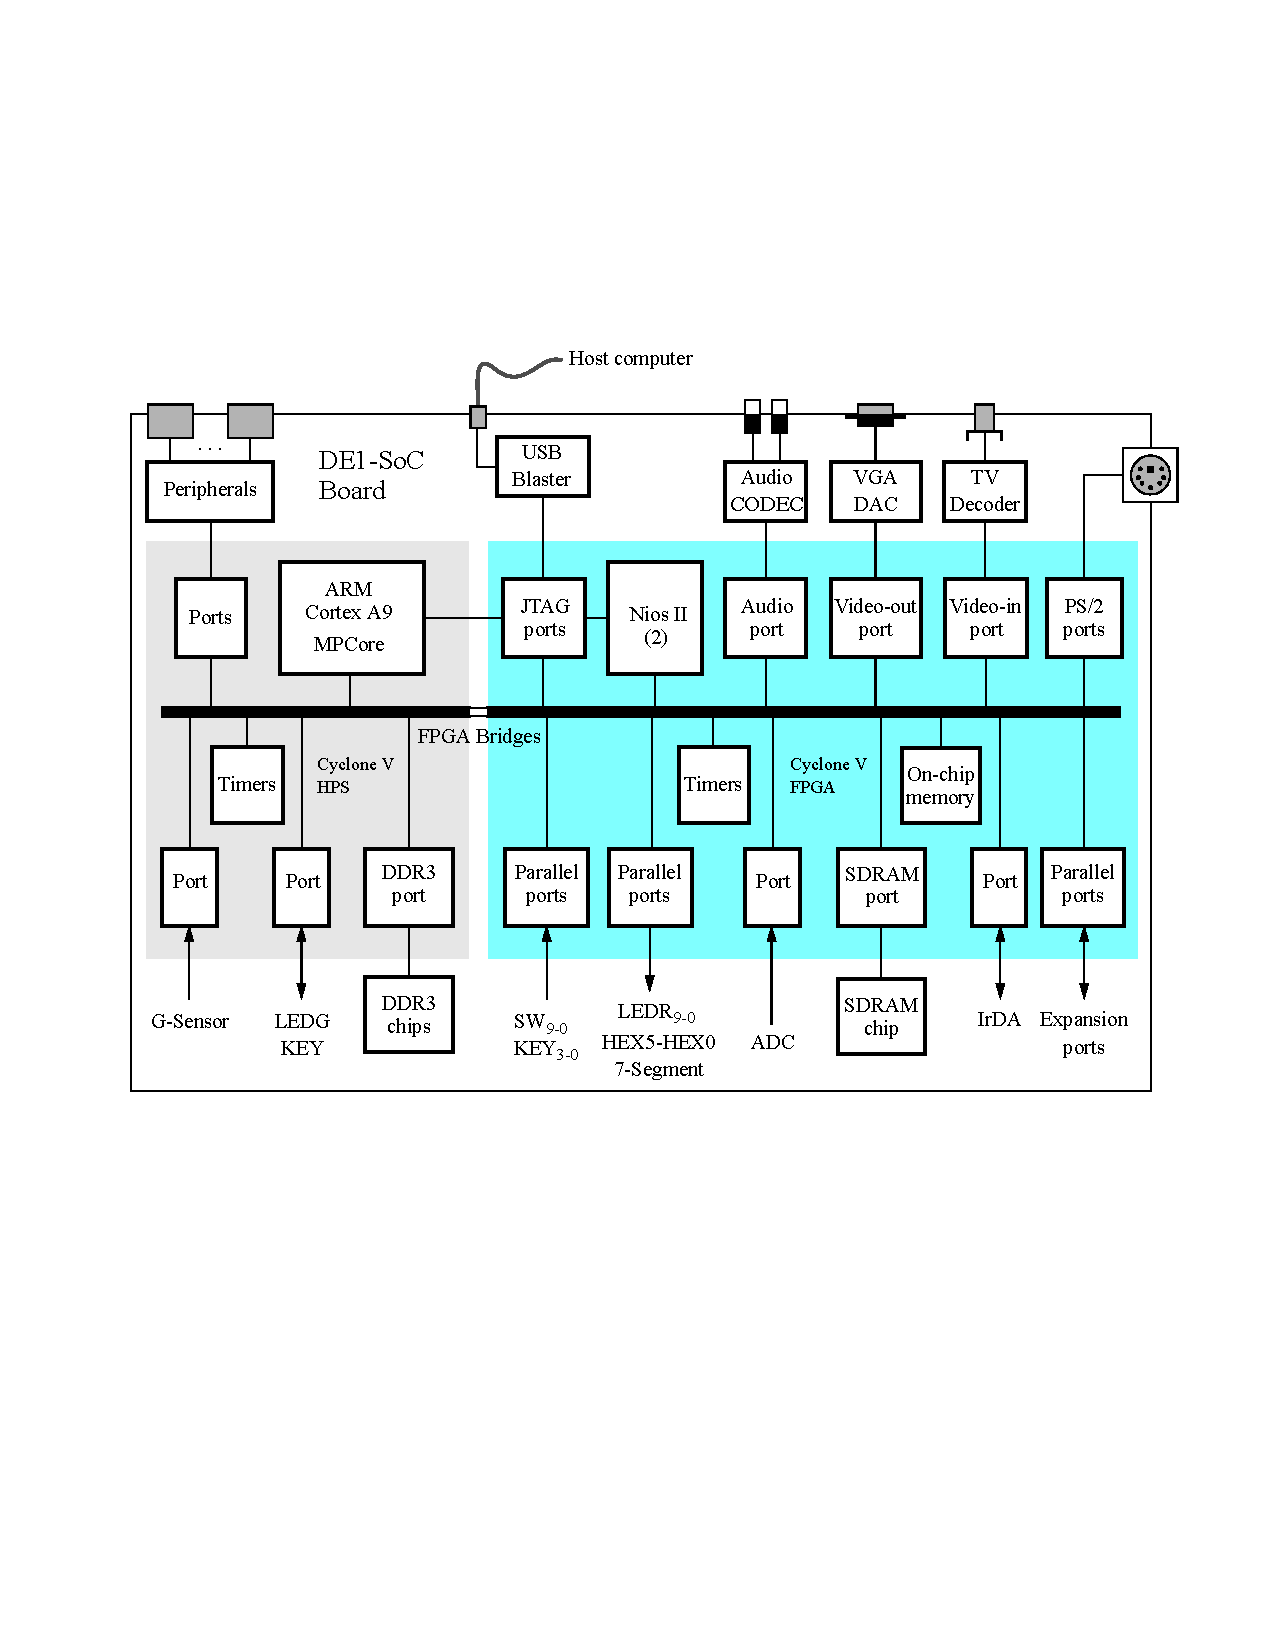
\includegraphics[height=.4\paperheight]{figures/fig_block_diagram.pdf}
   \end{center}
   \caption{Block diagram of the {\it \systemNameFull}.}
	\label{fig:block_diagram}
\end{figure}



\subsection{Nios\textsuperscript{\textregistered} II Processor}
\label{sec:nios2}
The Nios II processor is a 32-bit CPU that can be implemented
in an Altera FPGA device.  Two versions of the Nios II processor are available,
designated economy (/e) and fast (/f). The \systemName~includes two instances of the Nios II/f version, configured with floating-point hardware 
support.


An overview of the Nios II processor can be found in the document {\it Introduction to the
Nios~II Processor}, which is available in the
\texttt{Computer Organization System Design} section of the 
{\small \href{https://www.fpgacademy.org/tutorials.html} {FPGAcademy.org}} website.
An easy way to begin working with the \systemName~and the Nios~II
processor is to make use of a utility called the {\it \productNameMed{}}.  It
provides an easy way to assemble/compile Nios II programs 
written in either assembly language or the C language. The Monitor 
Program, which can be downloaded from the
{\small \href{https://www.fpgacademy.org/tools.html} {FPGAcademy.org}} website,
is an application program that 
runs on the host computer connected to the \DEBoard~board.  The Monitor Program can be 
used to control
the execution of code on Nios~II, list (and edit) the contents of processor registers, 
display/edit the contents of memory on the \DEBoard~board, and similar operations.
The Monitor Program includes the \systemName~as a predesigned system that can be
downloaded onto the \DEBoard~board, as well as several sample programs in assembly language and
C that show how to use the \systemName's peripherals.
Some images that show how the \systemName~is integrated with the 
Monitor Program are described in Section~\ref{sec:monitor_program}.

All of the I/O peripherals in the \systemName~are
accessible by the processor as memory mapped devices, 
using the address ranges that are given in the following subsections.



\subsection{Memory Components}

The \systemName~has DDR3 and SDRAM ports, as well as two memory modules implemented 
using the on-chip memory inside the FPGA. These memories are described below.

\subsubsection{SDRAM}
An SDRAM Controller in the FPGA provides an interface to the 64 MB synchronous dynamic RAM (SDRAM) 
on the \DEBoard~board, which is organized as 32M {\sf x} 16 bits. It is
accessible by the \processor~processor using word (32-bit), halfword (16-bit), or byte
operations, and is mapped to the address space {\sf 0x\baseAddressOffset 0000000} to {\sf 0x\baseAddressOffset 3FFFFFF}.



\subsubsection{DDR3 Memory}
\label{sec:ddr3}
A 1 GB DDR3 memory is connected to the HPS part of the
\FPGADeviceFamily~chip.  The memory is organized as 256M {\sf x} 32-bits, and is accessible 
using word accesses (32 bits), halfwords, and bytes. The {\processor} processor can access the 
DDR3 memory using the addresses space {\sf 0x40000000} to {\sf 0x7FFFFFFF}.  


\subsubsection{On-Chip Memory}
A 256 KB memory is implemented inside the FPGA, organized as 64K {\sf x} 32 bits. The 
{\processor} processor can access this memory using addresses in the range 
{\sf 0x\baseAddressOffset 8000000} to {\sf 0x\baseAddressOffset 803FFFF}. This
memory is used as a pixel buffer for the video-out and video-in ports.


\subsubsection{On-Chip Memory Character Buffer}
An 8 KB memory is implemented inside the FPGA for use as a character buffer for the video-out
port, which is described in Section~\ref{sec:video_out}.
The character buffer memory is organized as 8K {\sf x} 8 bits, and spans the {\processor}
address range {\sf 0x\baseAddressOffset 9000000} to {\sf 0x\baseAddressOffset 9001FFF}.



\subsection{Parallel Ports}
There are several parallel ports implemented in the FPGA that support input, output, and
bidirectional transfers of data between the \processor~processor and I/O peripherals. As 
illustrated in Figure~\ref{fig:parallel_port}, each parallel port is assigned a {\it Base}
address and contains up to four 32-bit registers. Ports that have output capability include a
writable {\it Data} register, and ports with input capability have a readable {\it
Data} register. Bidirectional parallel ports also include a {\it Direction} register that 
has the same bit-width as the {\it Data} register. Each bit in the {\it Data} register can be
configured as an input by setting the corresponding bit in the {\it Direction} register to 0,
or as an output by setting this bit position to~1. The {\it Direction} register is assigned the
address {\it Base} + 4.

\begin{figure}[h!]
   \begin{center}
       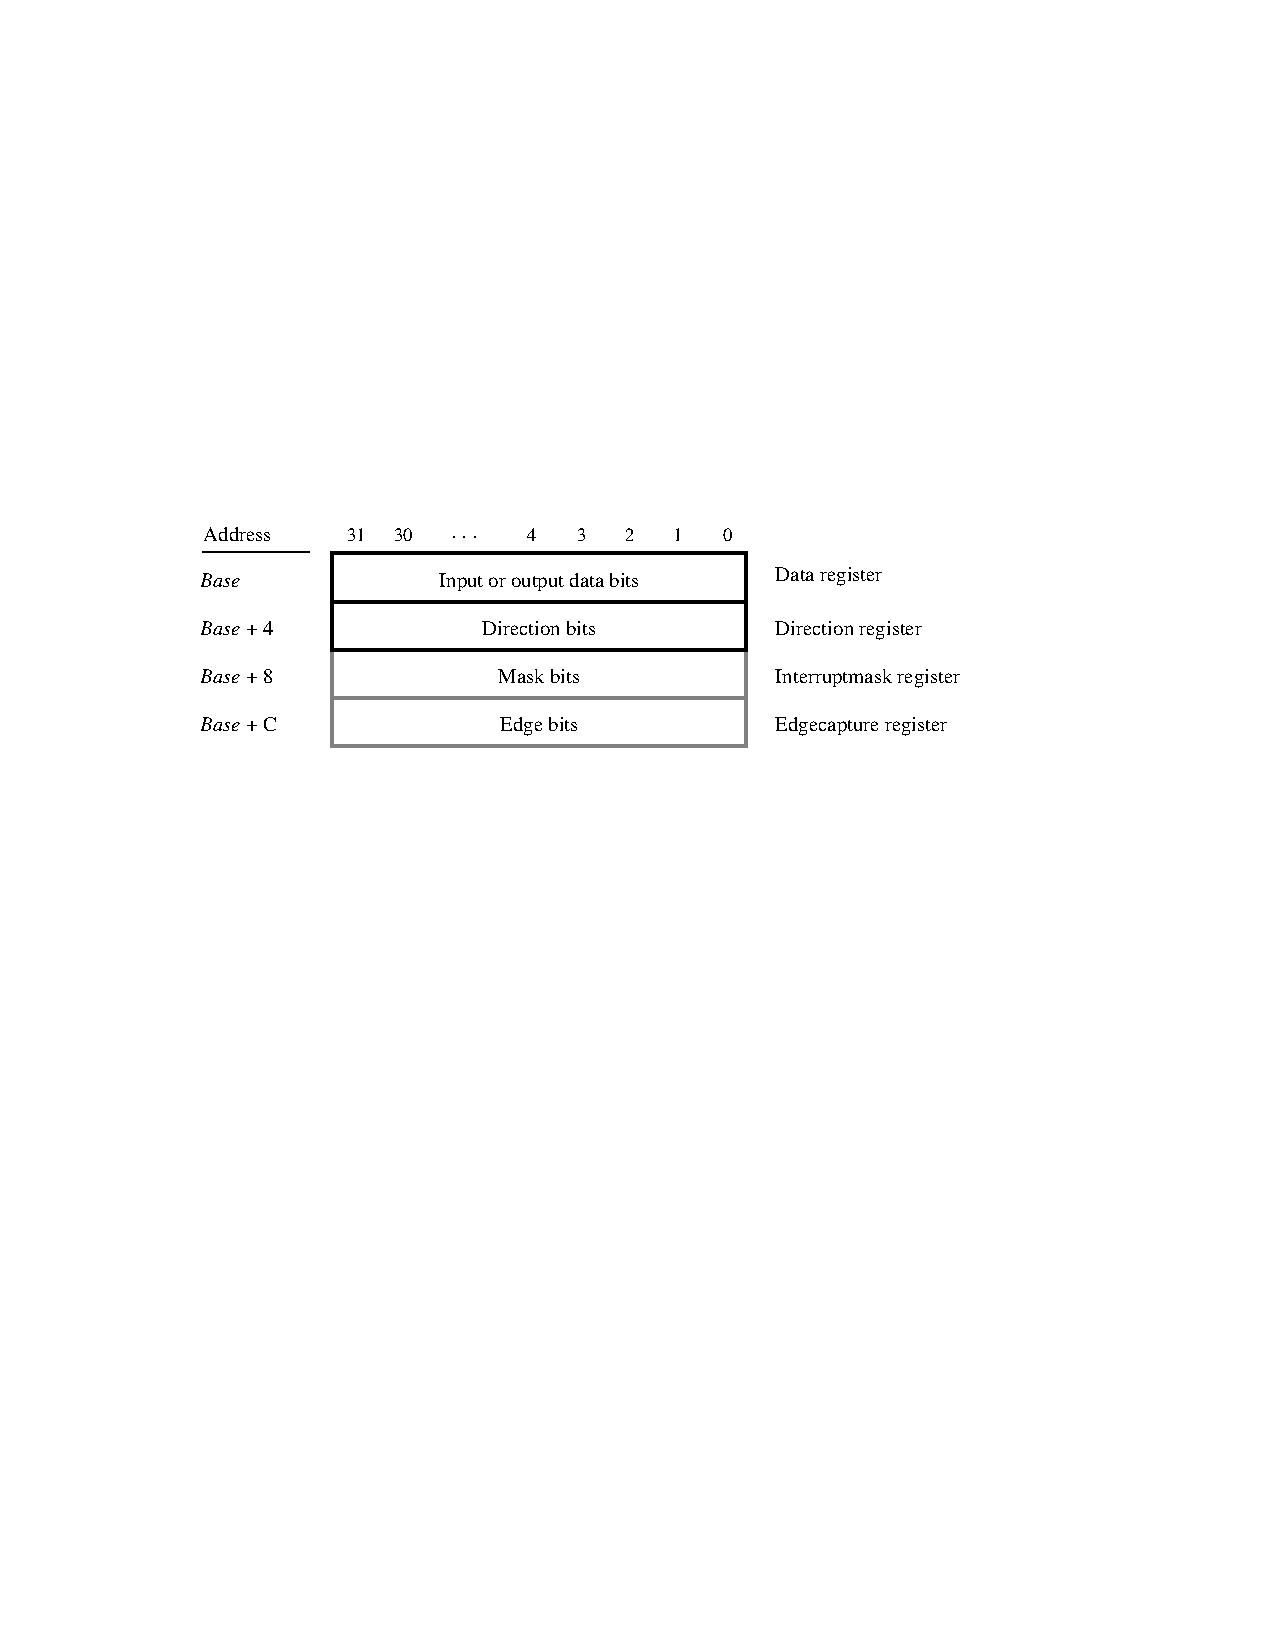
\includegraphics{../../../common/figs/FPGA_PP.pdf}
   \end{center}
   \caption{Parallel port registers in the {\it \systemNameFull}.}
	\label{fig:parallel_port}
\end{figure}

Some of the parallel ports have registers at addresses 
{\it Base} + 8 and {\it Base} + C, as indicated in Figure~\ref{fig:parallel_port}. These
registers are discussed in Section \ref{sec:exceptions}.



\subsubsection{Red LED Parallel Port}

The red lights {\it LEDR}$_{9-0}$ on the \DEBoard~board
are driven by an output parallel port, as illustrated in Figure \ref{fig:LED_port}. The port
contains a 10-bit {\it Data} register, which has the
address {\sf 0xFF200000}.  This register can be written or read by the processor using word 
accesses, and the upper bits not used in the registers are ignored.

\begin{figure}[h!]
   \begin{center}
       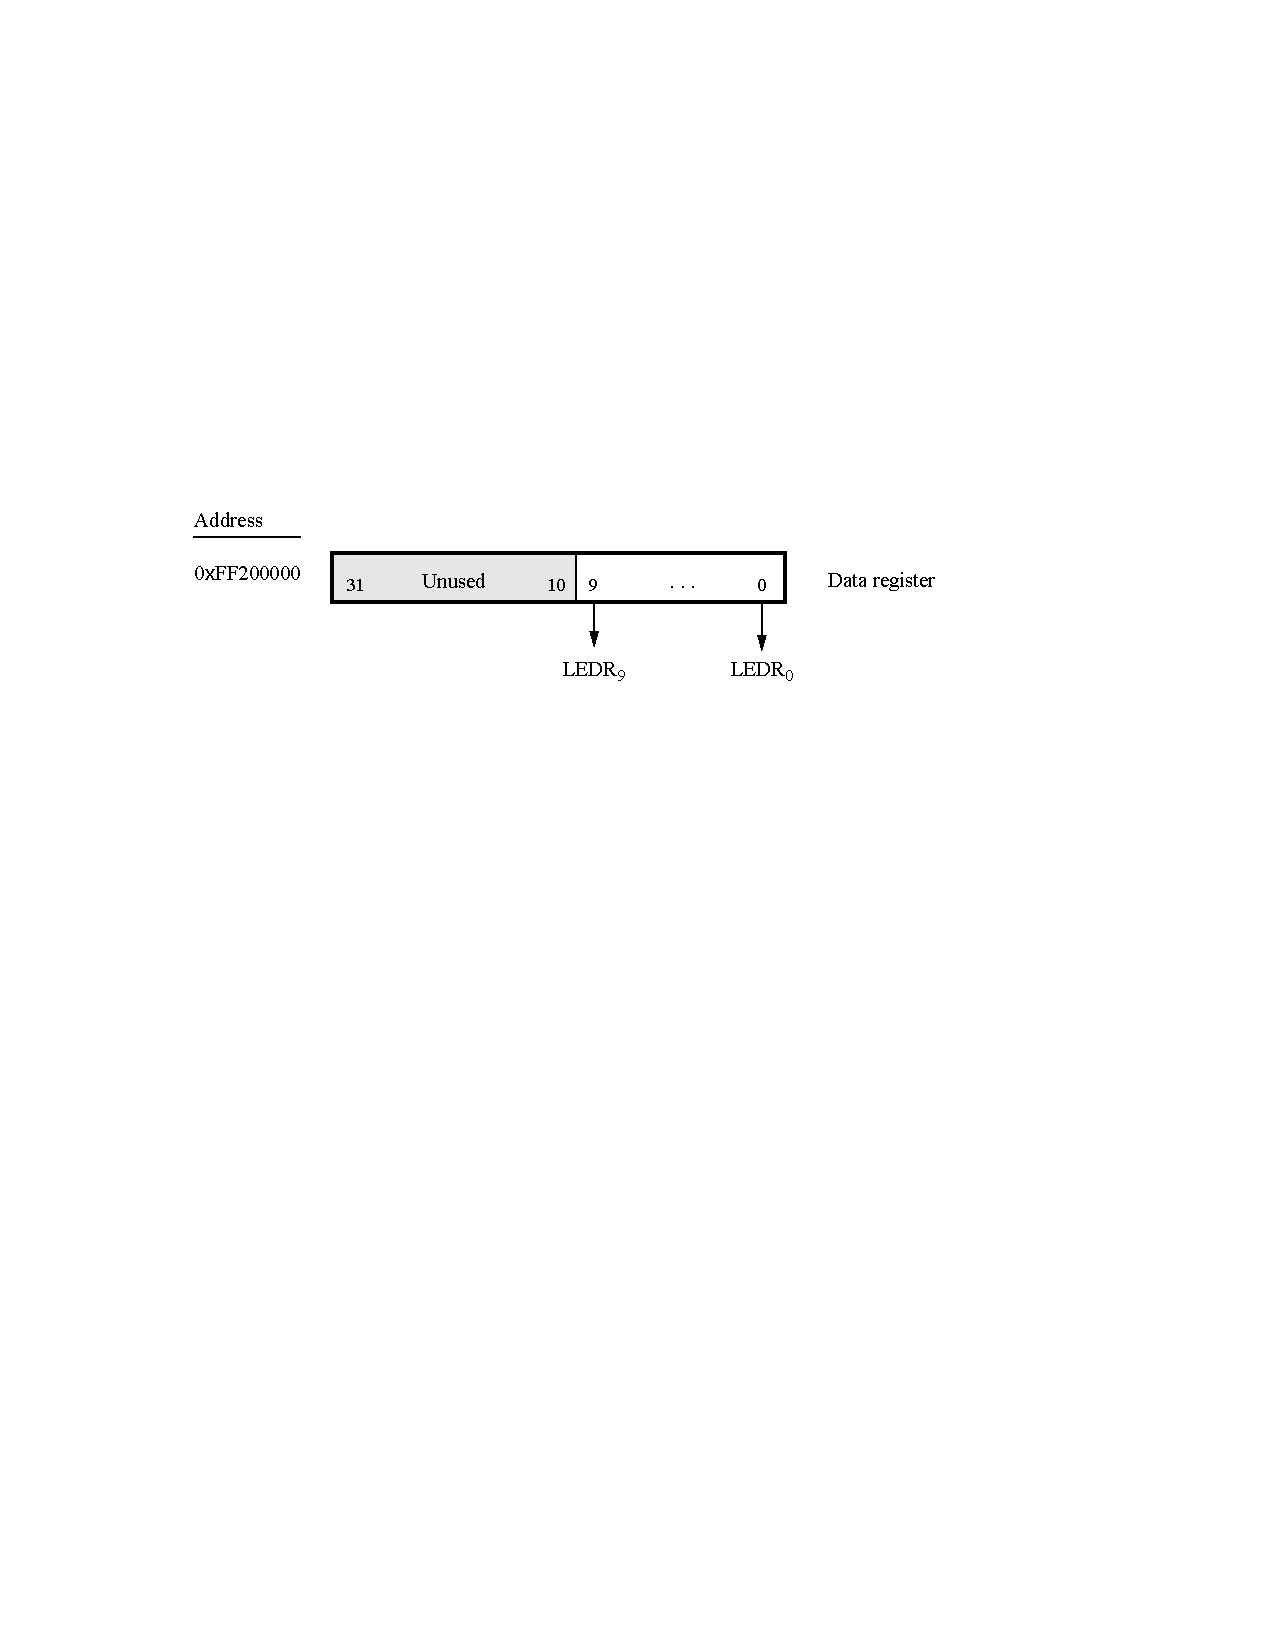
\includegraphics{../../../common/figs/FPGA_PP_Red_LEDs_10.pdf}
   \end{center}
   \caption{Output parallel port for {\it LEDR}.}
	\label{fig:LED_port}
\end{figure}



\subsubsection{7-Segment Displays Parallel Port}

There are two parallel ports connected to the 7-segment displays on the \DEBoard~board, each of
which comprises a 32-bit write-only {\it Data} register. As indicated in 
Figure \ref{fig:hex_segment_port}, the register at address {\sf 0xFF200020} 
drives digits {\it HEX3} to {\it HEX0}, and the register at 
address {\sf 0xFF200030} drives digits {\it HEX5} and
{\it HEX4}.  Data can be written into these two registers, and read back, by using word operations. 
This data directly controls the segments of each display, according to
the bit locations given in Figure \ref{fig:hex_segment_port}. The locations of segments 
6 to 0 in each seven-segment display on the \DEBoard~board is illustrated on the right side of the
figure.

\begin{figure}[h!]
   \begin{center}
       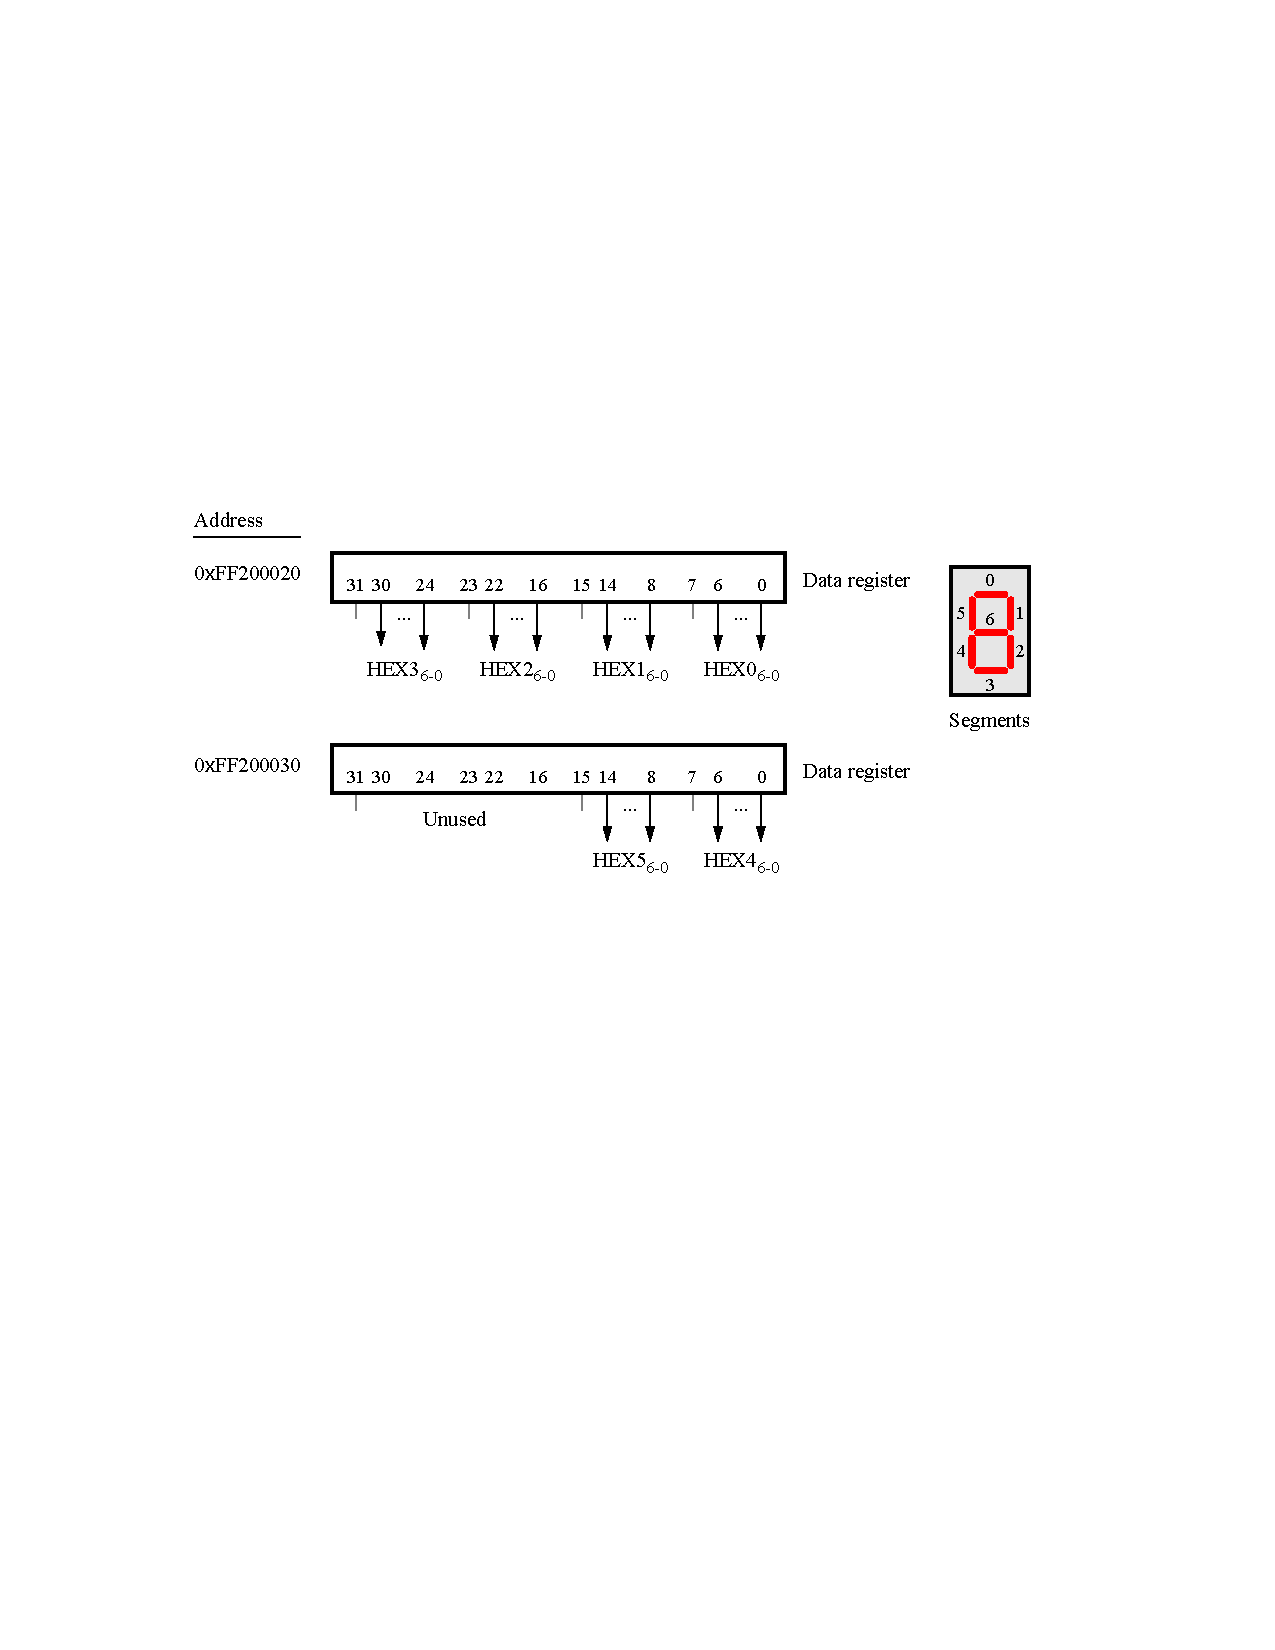
\includegraphics{../../../common/figs/FPGA_PP_7_Segs_6.pdf}
   \end{center}
   \caption{Bit locations for the 7-segment displays parallel ports.}
	\label{fig:hex_segment_port}
\end{figure}


\subsubsection{Slider Switch Parallel Port}

The {\it SW}$_{9-0}$ slider switches on the \DEBoard~board are connected to an input parallel
port.  As illustrated in Figure~\ref{fig:slider_port}, this port 
comprises a 10-bit read-only {\it Data} register, which is mapped to address {\sf 0xFF200040}.

\begin{figure}[h!]
   \begin{center}
       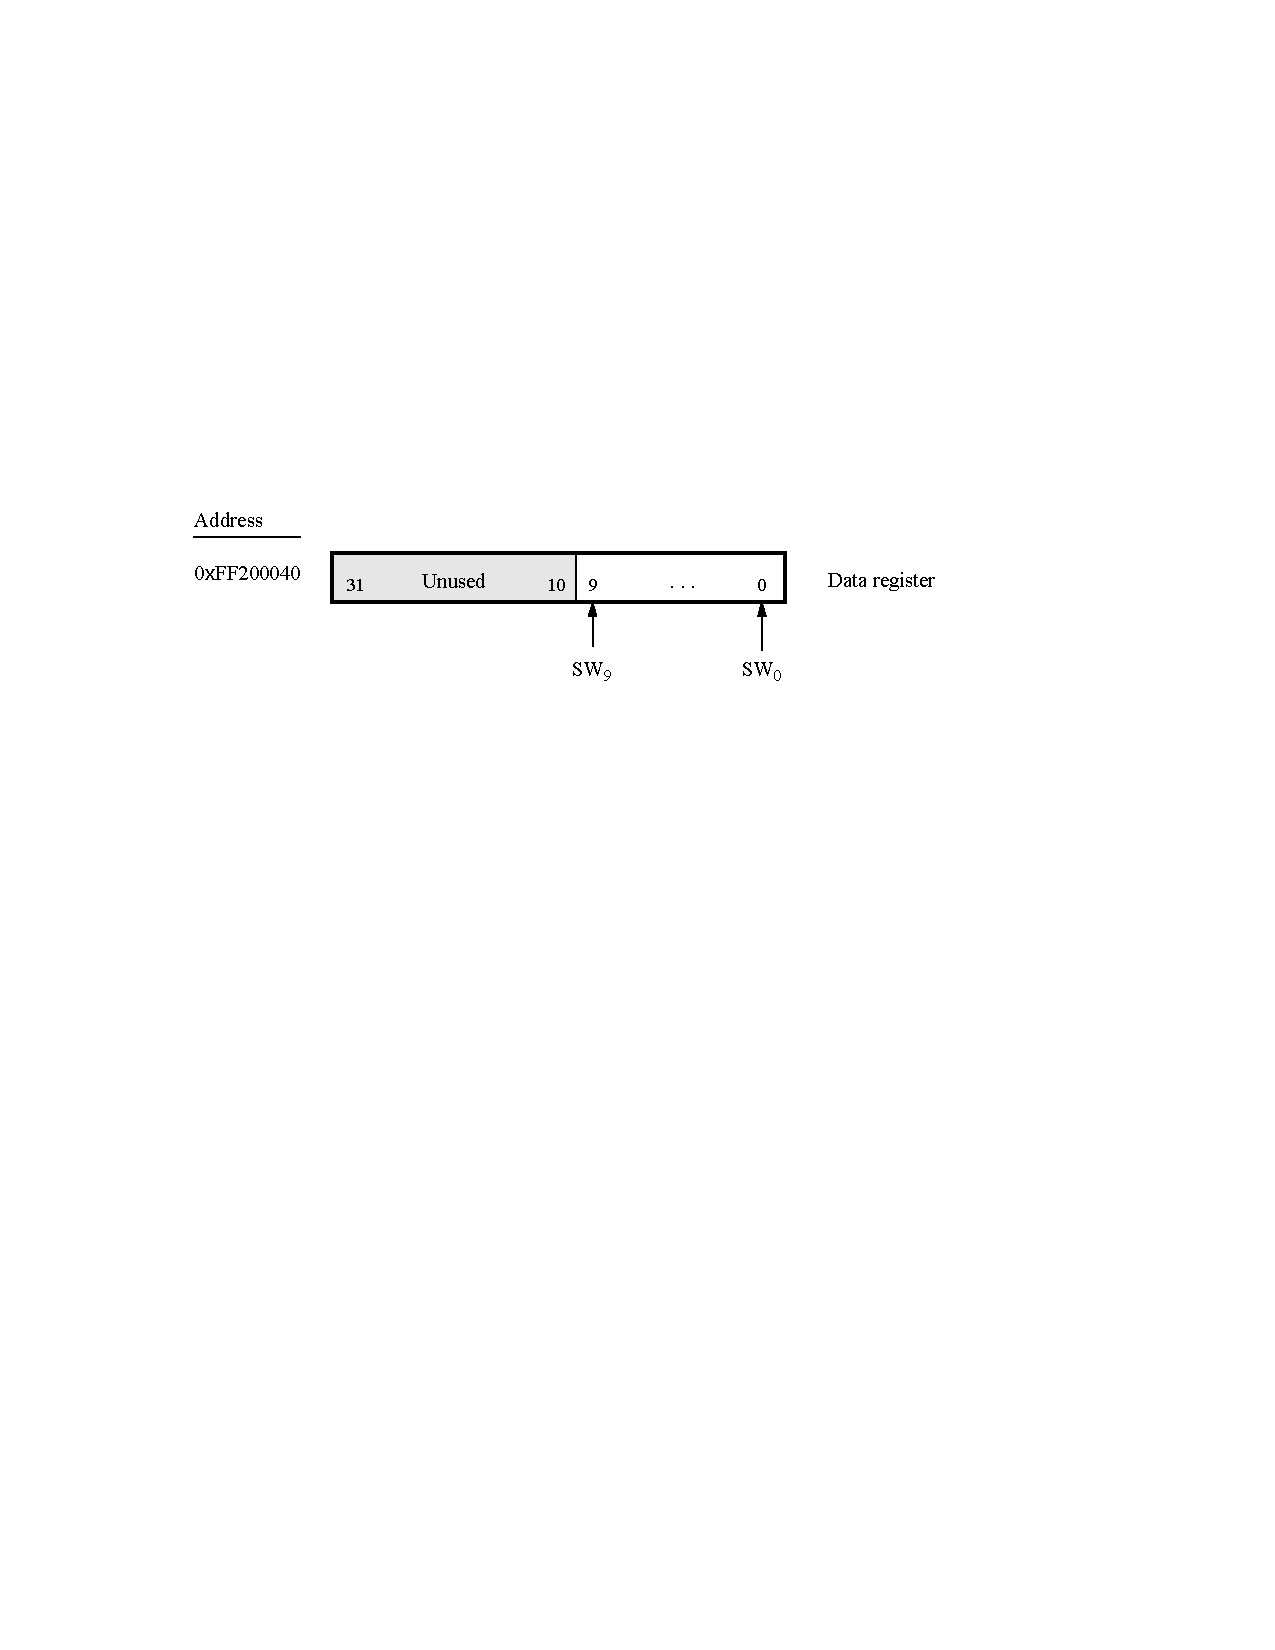
\includegraphics{../../../common/figs/FPGA_PP_Switches_10.pdf}
   \end{center}
   \caption{{\it Data} register in the slider switch parallel port.}
	\label{fig:slider_port}
\end{figure}


\subsubsection{Pushbutton Key Parallel Port}

The parallel port connected to the {\it KEY}$_{3-0}$ 
pushbutton switches on the \DEBoard~board comprises three 4-bit
registers, as shown in Figure \ref{fig:pushbutton_port}. These registers have 
the base address {\sf 0xFF200050} and can be accessed using word operations. 
The read-only {\it Data} register provides the values of the switches {\it KEY}$_{3-0}$. 
The other two registers shown in Figure \ref{fig:pushbutton_port}, at addresses
{\sf 0xFF200058} and {\sf 0xFF20005C}, are discussed in Section \ref{sec:exceptions}.
~\\
\begin{figure}[h!]
   \begin{center}
       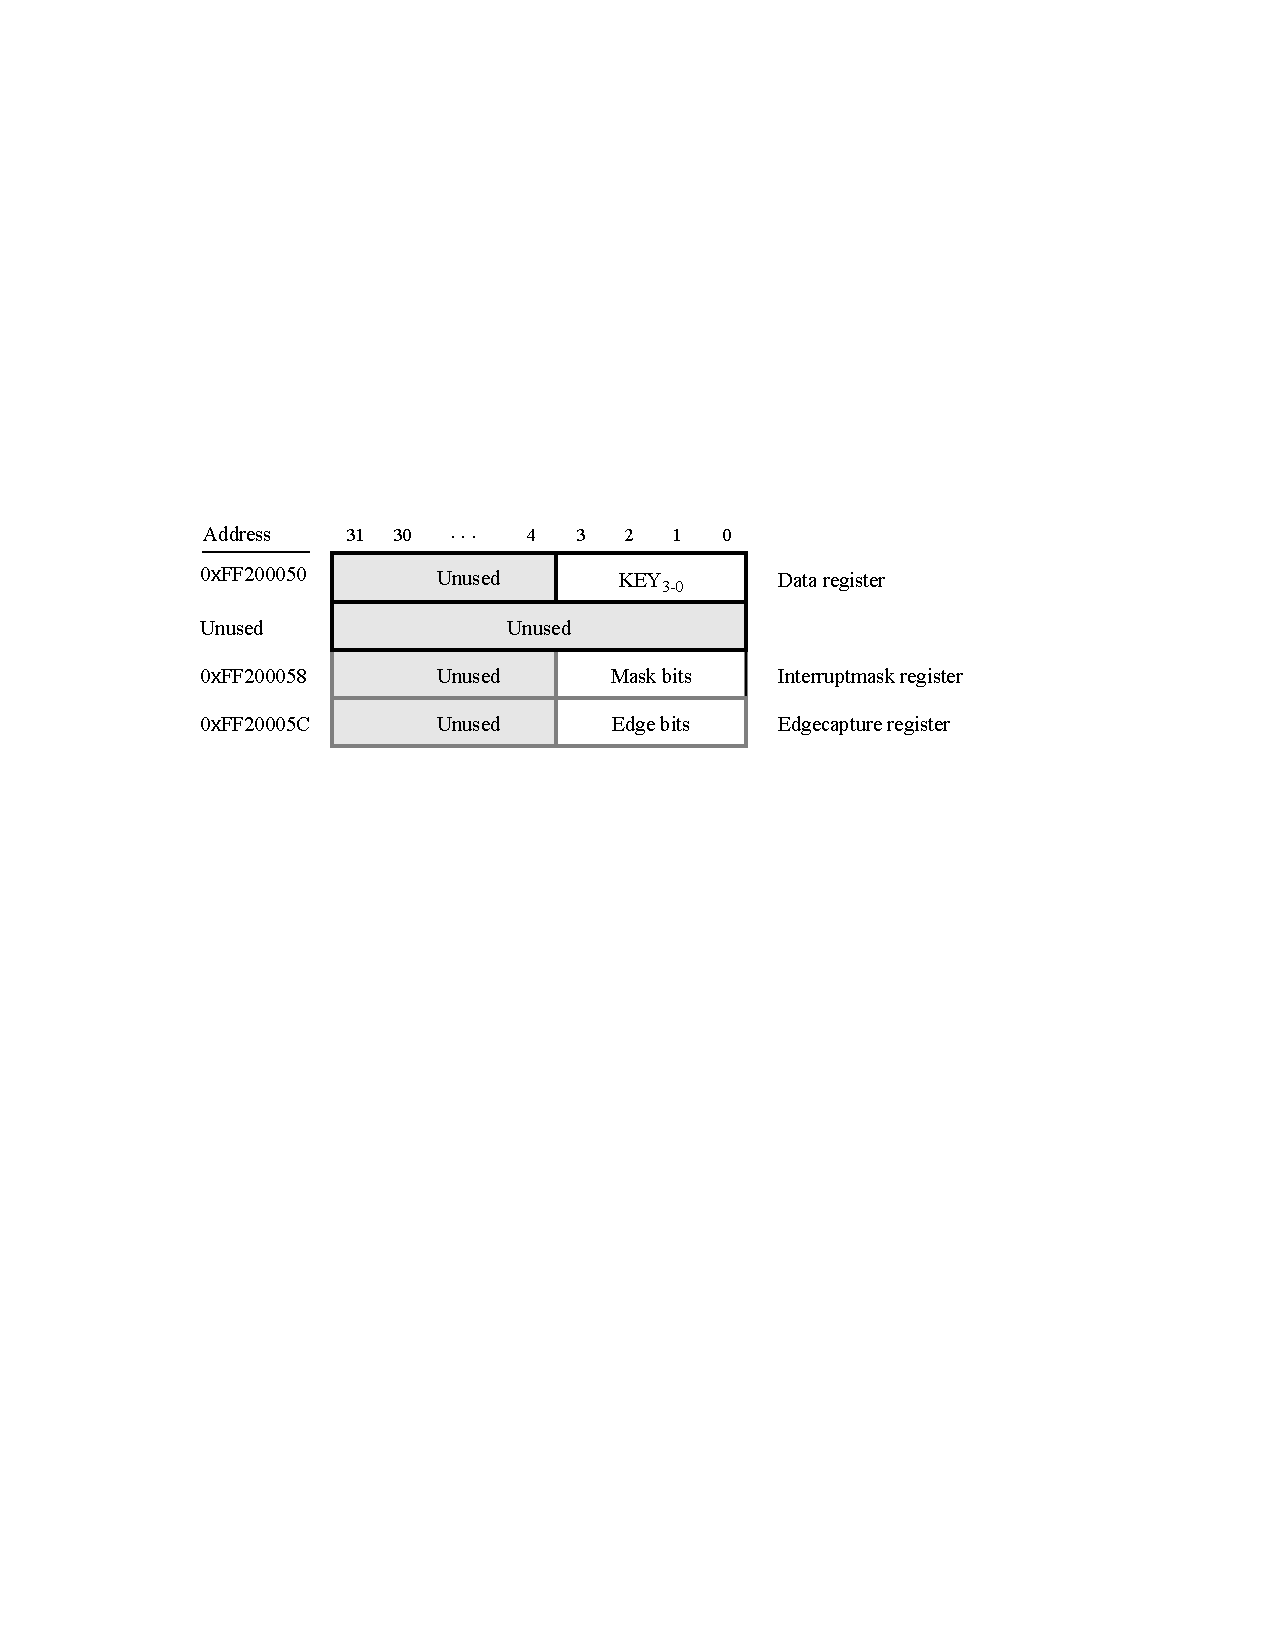
\includegraphics{../../../common/figs/FPGA_PP_Keys_4.pdf}
   \end{center}
   \caption{Registers used in the pushbutton parallel port.}
	\label{fig:pushbutton_port}
\end{figure}



\subsubsection{Expansion Parallel Port}

The {\it \systemNameFull} includes two bidirectional parallel ports that are connected to the
{\it \expansionPortA} and {\it \expansionPortB} 40-pin headers on the \DEBoard~board. These parallel ports
include the four 32-bit registers that were described previously for 
Figure~\ref{fig:parallel_port}. The base address of the port for \expansionPortA~is {\sf 0xFF200060},
and for \expansionPortB~is {\sf 0xFF200070}.  Figure~\ref{fig:expansion_port} gives a diagram of 
the 40-pin connectors on the \DEBoard~board, and shows how the respective parallel port {\it Data} register bits, 
$D_{31-0}$, are assigned to the pins on the connector. The figure shows that bit $D_0$ of
the parallel port is assigned to the pin at the top right corner of the
connector, bit $D_1$ is assigned below this, and so on. Note that some of the pins on
the 40-pin header are not usable as input/output connections, and are 
therefore not used by the parallel ports. Also, only 32 of the 36 data pins that appear on
each connector can be used.

\begin{figure}[h!]
   \begin{center}
       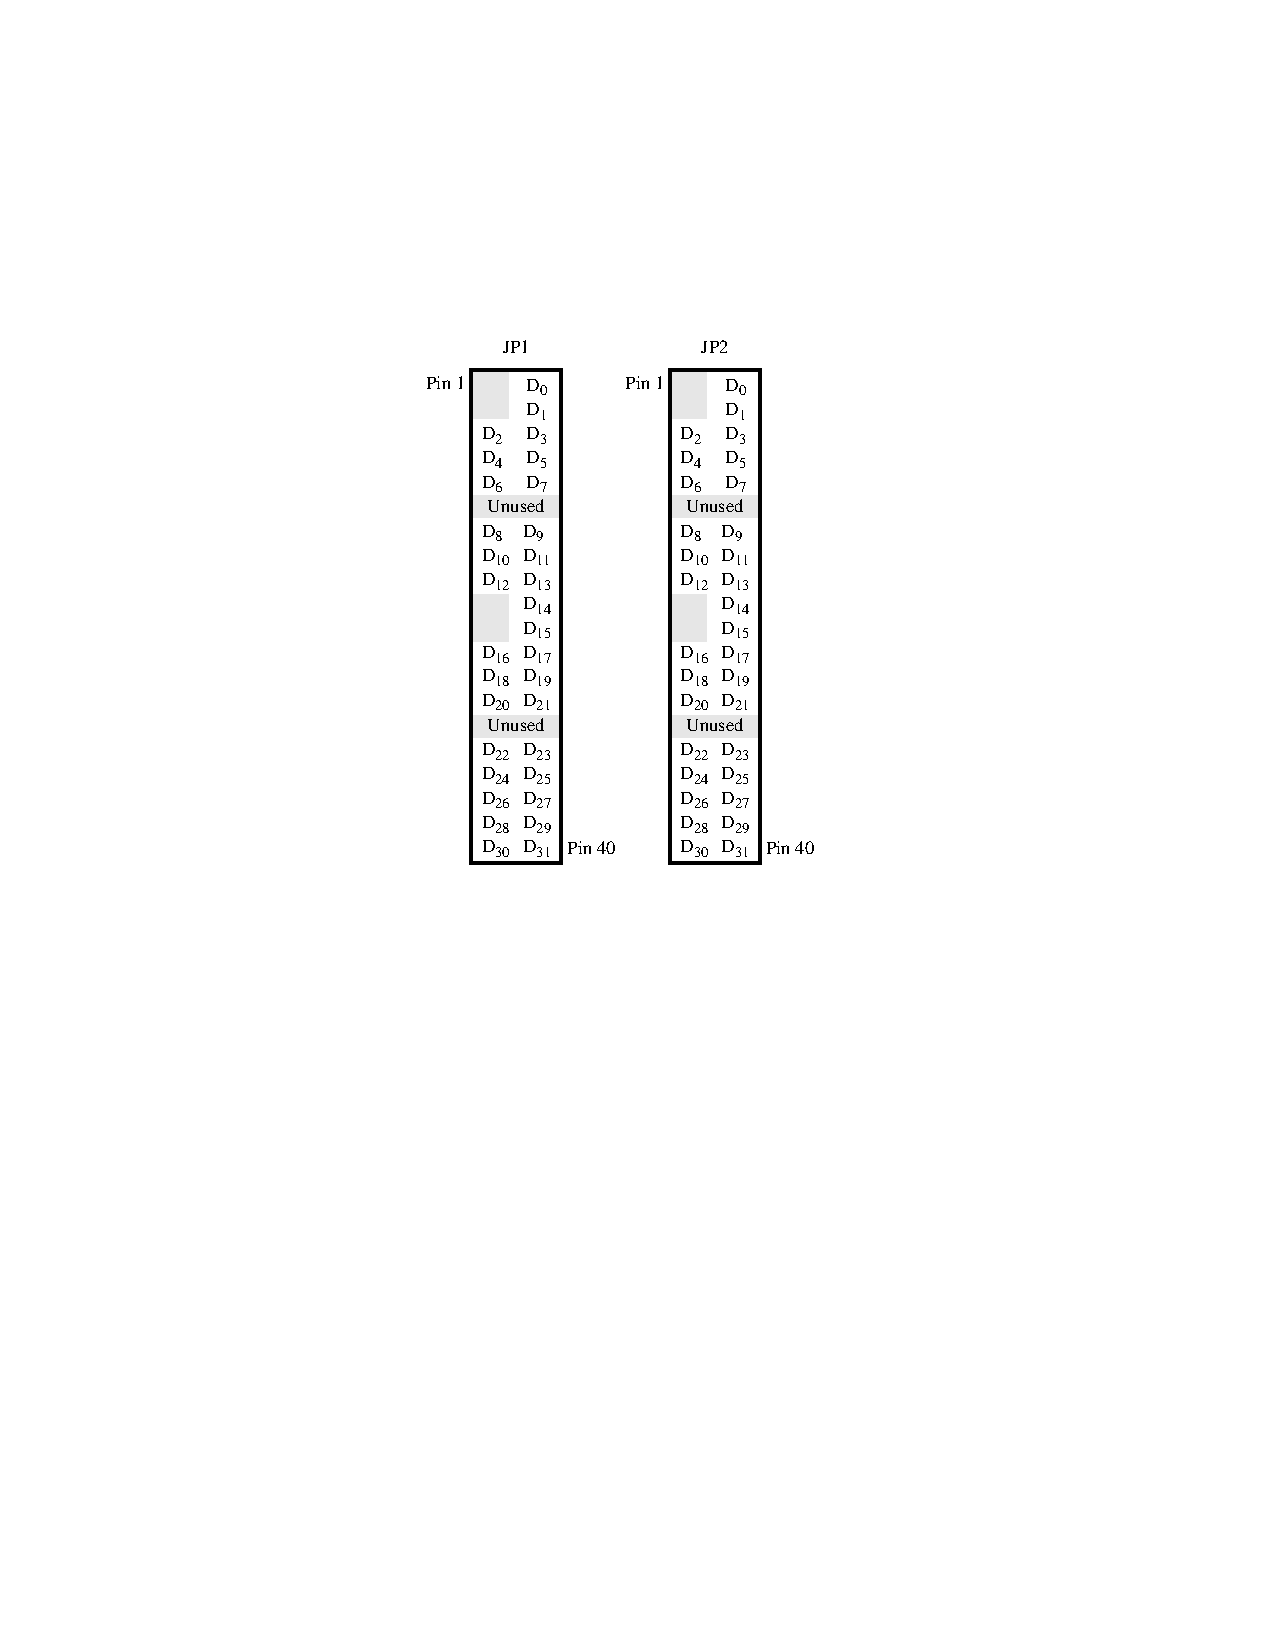
\includegraphics[trim={0 0 0 0.5cm},clip]{../../../common/figs/FPGA_PP_Expansion_Port.pdf}
   \end{center}
	\caption{Assignment of parallel port bits to pins on {\it \expansionPortA} and {\it \expansionPortB}.}
	\label{fig:expansion_port}
\end{figure}


\subsubsection{Using the Parallel Ports with Assembly Language Code and C Code}

The {\it \systemNameFull} provides a convenient platform for experimenting with {\processor}
assembly language code, or C code.  A simple example of such code is provided in the Appendix in
Listings \ref{lst:getting_started_s} and \ref{lst:getting_started_C}. Each of these
listing {\it includes} a file that specifies the memory-mapped addresses of all peripheral
devices in the {\it \systemNameFull}. These include files, called {\it address\_map\_niosV.s}
and {\it address\_map\_niosV.h}, are provided in Listings~\ref{lst:address_map_niosV_s}
and~\ref{lst:address_map_niosV_h}. These include files are also used in other code
samples described in this document.  

The code in Listing \ref{lst:getting_started_s} and \ref{lst:getting_started_C}
displays the values of the SW switches on the LED lights, and also
shows a rotating pattern on the LEDs. This pattern is shifted in a loop, using a software delay
to make the shifting slow enough to observe. The pattern can be changed to the values of the 
SW switches by pressing a pushbutton KEY. When a KEY is pressed, the program waits in a
loop until it is released and then continues to display the pattern.

The source code files shown in Listings \ref{lst:getting_started_s} and \ref{lst:getting_started_C}
are distributed as part of the  
\productNameMed{}. The files can be found under the heading {\it sample programs}, 
and are identified by the name {\it Getting Started}.




\subsection{JTAG* Port}
\label{sec:jtag_port}

The JTAG* port implements a communication link between the \DEBoard~board and its host computer.  
This link can be used by the Quartus\textsuperscript{\textregistered} Prime software to transfer FPGA programming files 
into the \DEBoard~board, and by the \productNameMed{}, discussed in 
Section~\ref{sec:monitor_program}.  The JTAG port also
includes a UART, which can be used to transfer character data between the host computer and
programs that are executing on the \processor~processor.
The programming interface 
of the JTAG UART consists of two 32-bit registers, as shown in Figure \ref{fig:jtag_port}. 
The register mapped to address {\sf 0xFF201000} is called the {\it Data}
register and the register mapped to address {\sf 0xFF201004} is called the {\it Control}
register.

\begin{figure}[h!]
   \begin{center}
       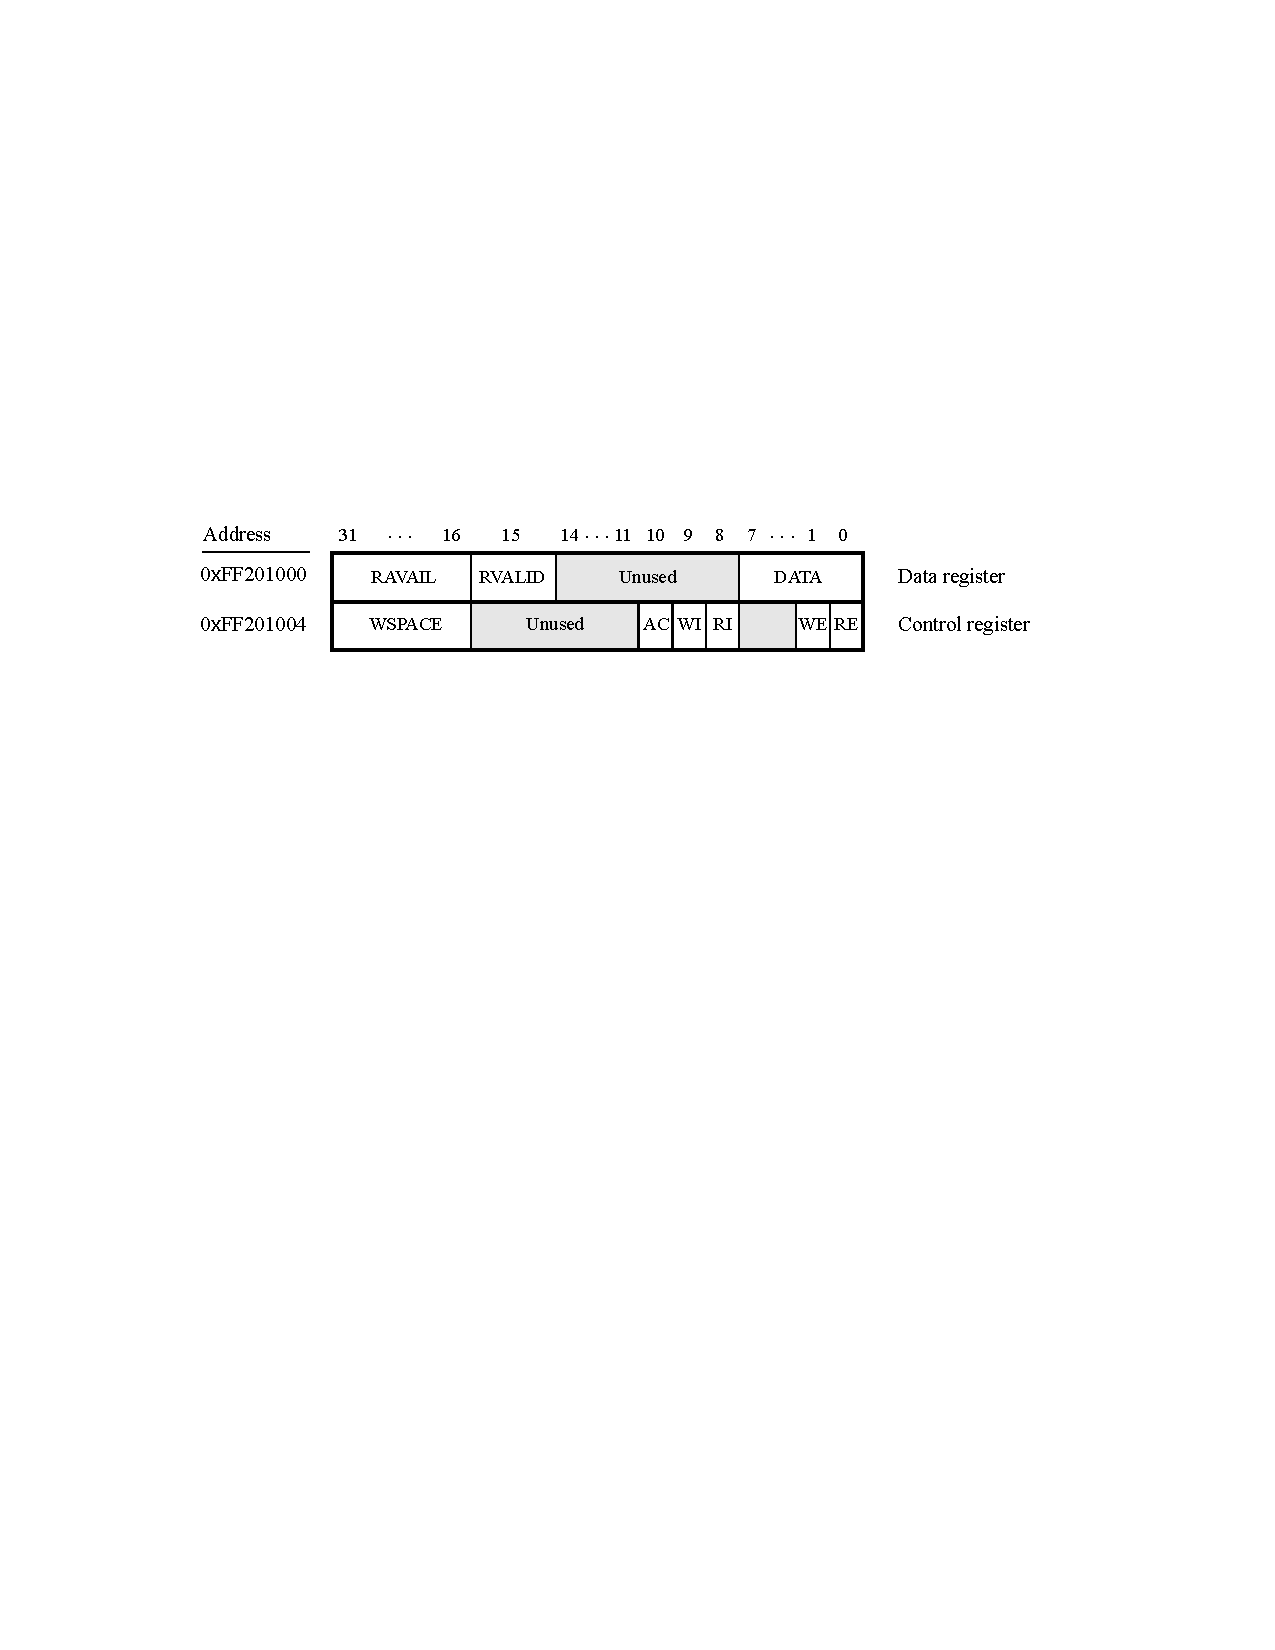
\includegraphics{../../../common/figs/FPGA_JTAG_UART.pdf}
   \end{center}
   \caption{JTAG UART registers.}
	\label{fig:jtag_port}
\end{figure}

When character data from the host computer is received by the JTAG UART 
it is stored in a 64-character FIFO.  The number of characters currently stored in this FIFO is
indicated in the field {\it RAVAIL}, which are
bits 31$-$16 of the {\it Data} register.  If the receive FIFO overflows, then
additional
data is lost. When data is present in the receive FIFO, then the value of {\it RAVAIL} will be 
greater than 0 and the value of bit 15, {\it RVALID}, will be 1. Reading the character at
the head of the FIFO, which is provided in bits $7-0$, decrements the value of {\it RAVAIL} 
by one and returns this decremented value as part of the read
operation. If no data is present in the receive FIFO, then {\it RVALID} will 
be set to 0 and the data in bits $7-0$ is undefined.

The JTAG UART also includes a 64-character FIFO that stores data 
waiting to be transmitted to the host computer. 
Character data is loaded into this FIFO by performing a write to bits 7$-$0
of the {\it Data} register in Figure \ref{fig:jtag_port}.  
Note that writing into this register has no effect 
on received data.  The amount of space, {\it WSPACE}, currently available in the transmit FIFO is 
provided in bits 31$-$16 of the {\it Control} register.  If
the transmit FIFO is full, then any characters written to the {\it Data} register will be lost.

Bit 10 in the {\it Control} register, called {\it AC}, has the value 1 if the JTAG UART has been
accessed by the host computer. This bit can be used to check if a working connection to
the host computer has been established. The {\it AC} bit can be cleared to 0 by writing a 1
into it.

The {\it Control} register bits {\it RE}, {\it WE}, {\it RI}, and {\it WI} are described 
in Section \ref{sec:exceptions}.

\subsubsection{Using the JTAG* UART with Assembly Language Code and C Code}

Listings \ref{lst:jtag_uart_s} and \ref{lst:jtag_uart_C} give simple examples of 
assembly language and C code, respectively, that use the JTAG UART. Both versions of the
code perform the same function, which is to first send an ASCII string to the JTAG UART,
and then enter an endless loop. In the loop, the code reads character data that has 
been received by the JTAG UART, and echoes this data back to the UART for transmission. In
the {\it CPUlator} simulator, there is a JTAG window that allows text to be typed and
echoed. If the program is executed by using the \productNameMed{}, then any keyboard character that 
is typed into the {\it Terminal Window} of the Monitor Program will be 
echoed back, causing the character to appear in the {\it Terminal Window}.

The source code files shown in Listings \ref{lst:jtag_uart_s} and \ref{lst:jtag_uart_C}
are made available as part of the  
\productNameMed{}. The files can be found under the heading {\it sample programs}, 
and are identified by the name {\it JTAG UART}.



\subsection{Interval Timers}
\label{sec:interval_port}

The {\it \systemNameFull} includes a timer module implemented in the FPGA that can be used by
the \processor~processor. This timer can be loaded with a preset value, and then counts down to 
zero using a 100-MHz clock. The programming interface 
for the timer includes six 16-bit registers, as illustrated in Figure~\ref{fig:interval_port}.  
The 16-bit register at address {\sf 0xFF202000} provides status information about the timer,
and the register at address {\sf 0xFF202004} allows control settings to be made.  The bit 
fields in these registers are described below:

\begin{itemize}
\item
{\it TO} provides a timeout signal which is set to 1 by the timer when it 
has reached a count value of zero.  The {\it TO} bit can be reset by writing a 0 into it. 
\item 
{\it RUN} is set to 1 by the timer whenever it is currently counting. Write 
operations to the status halfword do not affect the value of the {\it RUN} bit. 

\item 
{\it ITO} is used for generating interrupts, which are discussed in section \ref{sec:exceptions}.

\begin{figure}[h!]
   \begin{center}
       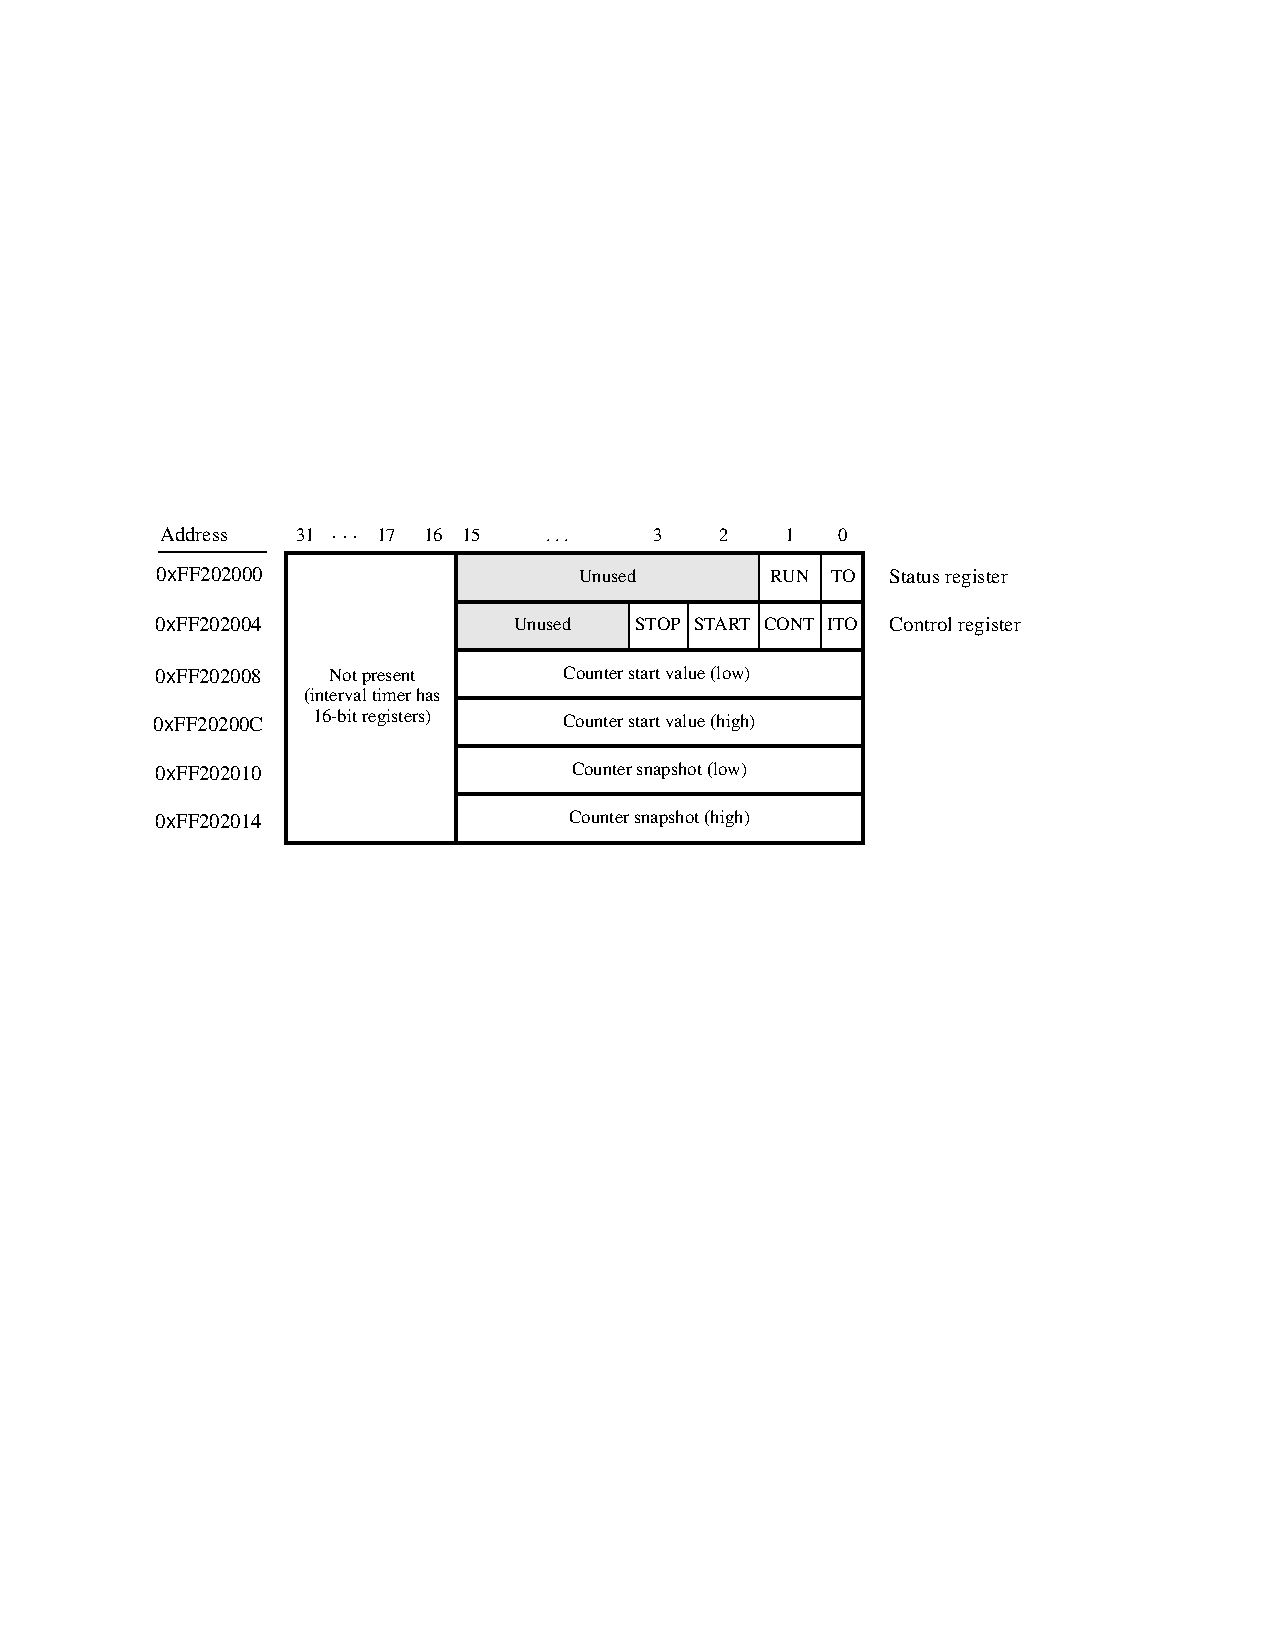
\includegraphics{../../../common/figs/FPGA_Interval_Timers.pdf}
   \end{center}
   \caption{Interval timer registers.}
	\label{fig:interval_port}
\end{figure}

\item
{\it CONT} affects the continuous operation of the timer.  When the timer reaches
a count value of zero it automatically reloads the specified starting count value. If 
{\it CONT} is set to 1, then the timer will continue counting down automatically.
But if {\it CONT} $=0$, then the timer will stop after it has reached a count value of 0. 

\item
({\it START}/{\it STOP}) is used to commence/suspend the operation of the 
timer by writing a 1 into the respective bit.
\end{itemize}

The two 16-bit registers at addresses {\sf 0xFF202008} and {\sf 0xFF20200C}
allow the period of the timer to be changed by
setting the starting count value.  The default setting gives a timer period of 125 msec. 
To achieve this period, the starting value of the count is
100 MHz $\times$ 125 msec $=12.5\times10^6$. It is possible to capture a snapshot of the 
counter value at any time by performing a write to address {\sf 0xFF202010}. This write
operation causes the current 32-bit counter value to be stored into the two 16-bit timer
registers at addresses {\sf 0xFF202010} and {\sf 0xFF202014}. These registers can then be
read to obtain the count value.

A second interval timer, which has an identical interface to the one described above, is also 
available in the FPGA, starting at the base address {\sf 0xFF202020}.


Each Nios II processor has exclusive access to two interval timers.
\subsection{G-Sensor}
\label{sec:G_sensor}
The {\it \systemNameFull} includes a 3D accelerometer (G-sensor) that is connected to the HPS.
The \processor~processor can access this device via an I2C serial interface at the base
address {\sf 0xFFC04000}. More details can be found in the
tutorial {\it Using the Accelerometer on DE-series Boards}.



\subsection{Floating-point Hardware}
\label{sec:fp}

The Nios~II processor in the \systemName~includes hardware support for
floating-point addition, subtraction, multiplication, and division. To use this support in
a C program, variables must be declared with the type {\it float}. A simple example of 
such code is given in Listing~\ref{lst:fp}. When this code is compiled, it is necessary to
pass the special argument {\sf -mcustom-fpu-cfg=60-2} to the C compiler, to instruct it to 
use the floating-point hardware support.


\subsection{System ID}

The system ID module provides a unique value that identifies the \systemName~
system.  The host computer connected to the \DEBoard~board can query the
system ID module by performing a read operation through the JTAG port. The host computer can 
then check the value of the returned identifier to confirm that the \systemName~has 
been properly downloaded onto the \DEBoard~board.  This process allows debugging tools on the 
host computer, such as the \productNameMed{}, to verify that the 
\DEBoard~board contains the required computer system before attempting to execute code 
that has been compiled for this system.


% Section: Exceptions and Interrupts
\section{Exceptions and Interrupts}
\label{sec:exceptions}

The reset address of the Nios II processor in the \systemName~is set to
{\sf 0x00000000}. The address used for all other general exceptions, such as 
divide by zero, and hardware IRQ interrupts 
is {\sf 0x00000020}. Since the Nios II processor uses the same address for general
exceptions and hardware IRQ interrupts, the
Exception Handler software must determine the source of the exception by examining the
appropriate processor status register. Table \ref{tab:irq}
gives the assignment of IRQ numbers to each of the I/O peripherals in the \systemName.
The rest of this section describes the interrupt behavior associated with the interval
timer, parallel ports, and serial ports in the \systemName. 



\begin{table}[h]
    \begin{center}
    \begin{tabular}{l|l}
            \textbf{I/O Peripheral} &
            \textbf{IRQ \#}
        \\\hline
            Interval timer & 0
        \\
            Pushbutton switch parallel port & 1
        \\
            Second Interval timer & 2
        \\
            Audio port & 6
        \\
            PS/2 port & 7
        \\
            JTAG port & 8
        \\
						IrDA port & 9
				\\
            Serial port & 10
        \\
            JP1 Expansion parallel port & 11
        \\
            JP2 Expansion parallel port & 12
        \\
						PS/2 port dual & 23
				\\
    \end{tabular}
    \caption{Hardware IRQ interrupt assignment for the DE1-SoC Computer.}
	 \label{tab:irq}
    \end{center}
\end{table}
\newpage

\subsection{Interrupts from Parallel Ports}

Parallel ports were illustrated in Figure~\ref{fig:parallel_port}, which is reproduced 
as Figure~\ref{fig:parallel_port_int}.
As the figure shows, parallel ports that support interrupts include two related registers 
at the addresses {\it Base} + 8 and {\it Base} + C.
The {\it Interruptmask} register, which has the address {\it Base} + 8, specifies whether 
or not an interrupt signal should be sent to the \GIC~when the data present at
an input port changes value.  Setting a bit location in this register to 1 allows 
interrupts to be generated, while setting the bit to 0 prevents interrupts. 
Finally, the parallel port may contain an {\it Edgecapture} register at address
{\it Base} + C.  Each bit in this register has the value 1 if the 
corresponding bit location in the parallel port has changed its value from 0 to 1.
A bit in the {\it Edgecapture} register can be cleared to 0
by writing a 1 into the corresponding bit position, which clears any associated interrupt. 

\begin{figure}[h!]
   \begin{center}
       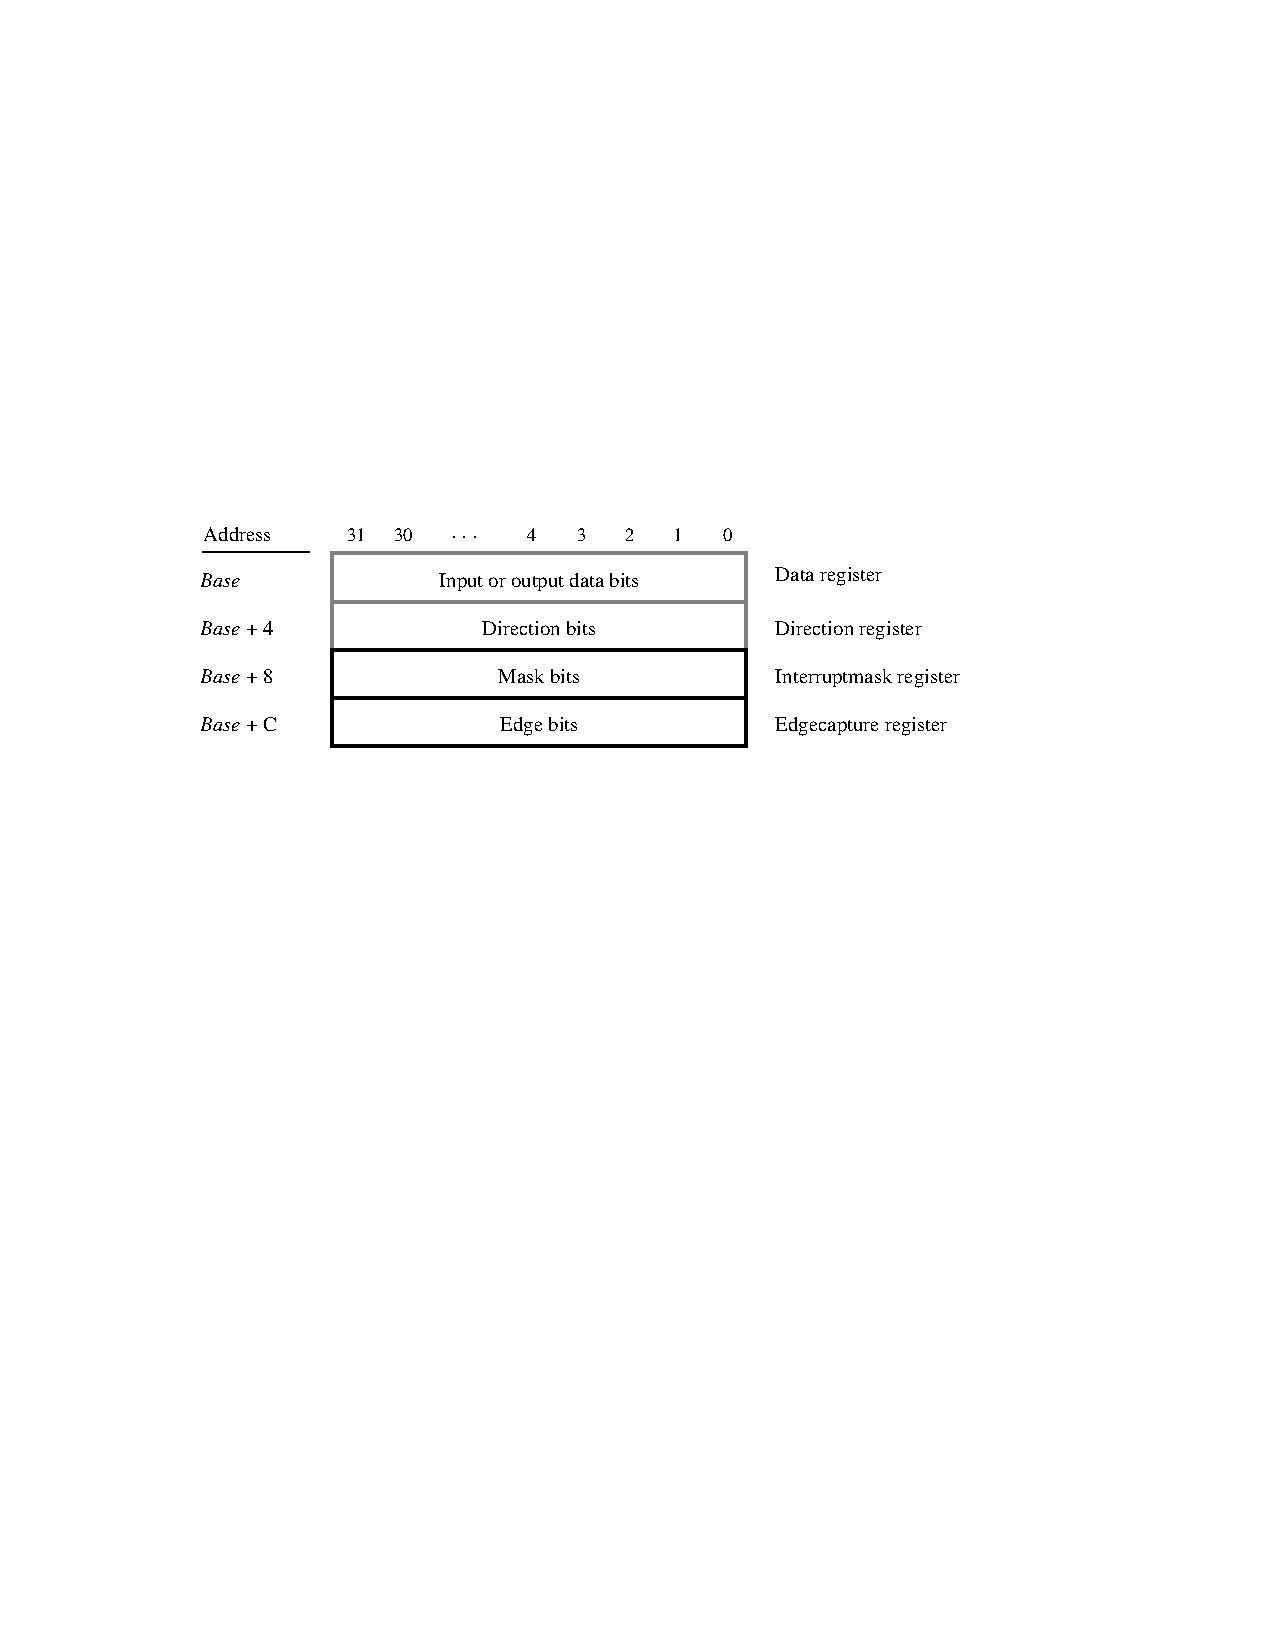
\includegraphics{../../../common/figs/Interrupts_FPGA_PP.pdf}
   \end{center}
   \caption{Registers used for interrupts from the parallel ports.}
	\label{fig:parallel_port_int}
\end{figure}



\subsubsection{Interrupts from the Pushbutton KEY Port}

Figure \ref{fig:pushbutton_port}, reproduced as Figure \ref{fig:pushbutton_port_int},
shows the registers associated with the pushbutton KEY port. 
The {\it Interruptmask} register allows interrupts to be generated when a key is
pressed. Interrupts can be enabled individually for each key by setting its 
{\it Interruptmask} bit to 1.  When a key is pressed, the corresponding bit in the 
{\it Edgecapture} register is set to 1 by the parallel port. This bit remains 1
until cleared to 0 by software.  An interrupt service routine can read the {\it Edgecapture} 
register to determine which key/s has/have been pressed.  An {\it Edgecapture} register bit can 
be cleared by writing a logic value 1 into the bit position.  Clearing the
bit resets the corresponding interrupt signal being sent to the \GIC.

\begin{figure}[h!]
   \begin{center}
       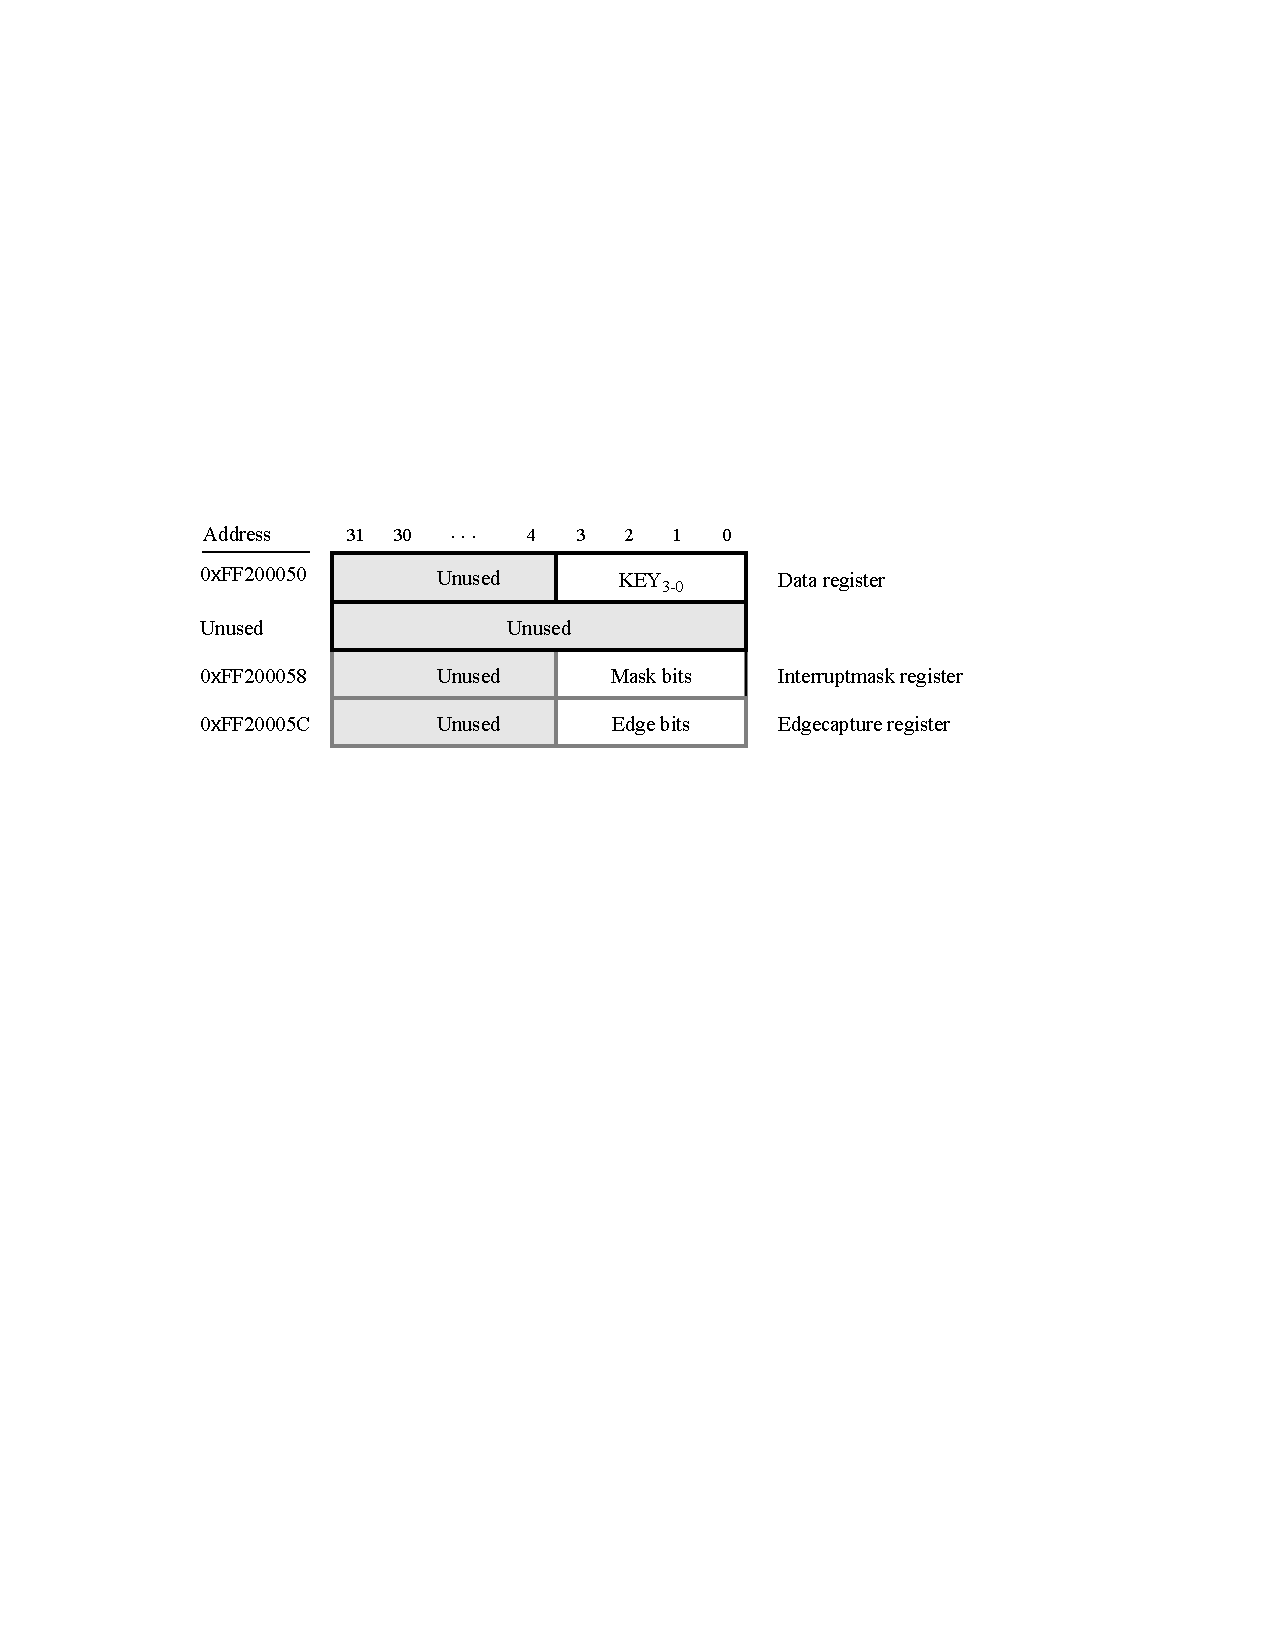
\includegraphics{../../../common/figs/FPGA_PP_Keys.pdf}
   \end{center}
   \caption{Registers used for interrupts from the pushbutton KEY port.}
	\label{fig:pushbutton_port_int}
\end{figure}


\subsection{Interrupts from the JTAG* UART}

Figure \ref{fig:jtag_port}, reproduced as Figure \ref{fig:jtag_port_int}, shows the {\it Data} 
and {\it Control} registers of the JTAG UART. As we said in Section~\ref{sec:jtag_port}, 
{\it RAVAIL} in the {\it Data} register gives the number of characters that 
are stored in the receive 
FIFO, and {\it WSPACE} gives the amount of unused space that is available in the transmit FIFO. 
The {\it RE} and {\it WE} bits in Figure \ref{fig:jtag_port_int}
are used to enable processor interrupts associated with the receive and transmit FIFOs. 
When enabled, interrupts are generated when {\it RAVAIL} for the receive FIFO, 
or {\it WSPACE} for the transmit FIFO, exceeds 7. Pending interrupts are indicated in the 
Control register's {\it RI} and {\it WI} bits, and can be cleared by writing or reading data
to/from the JTAG UART.

\begin{figure}[h!]
   \begin{center}
       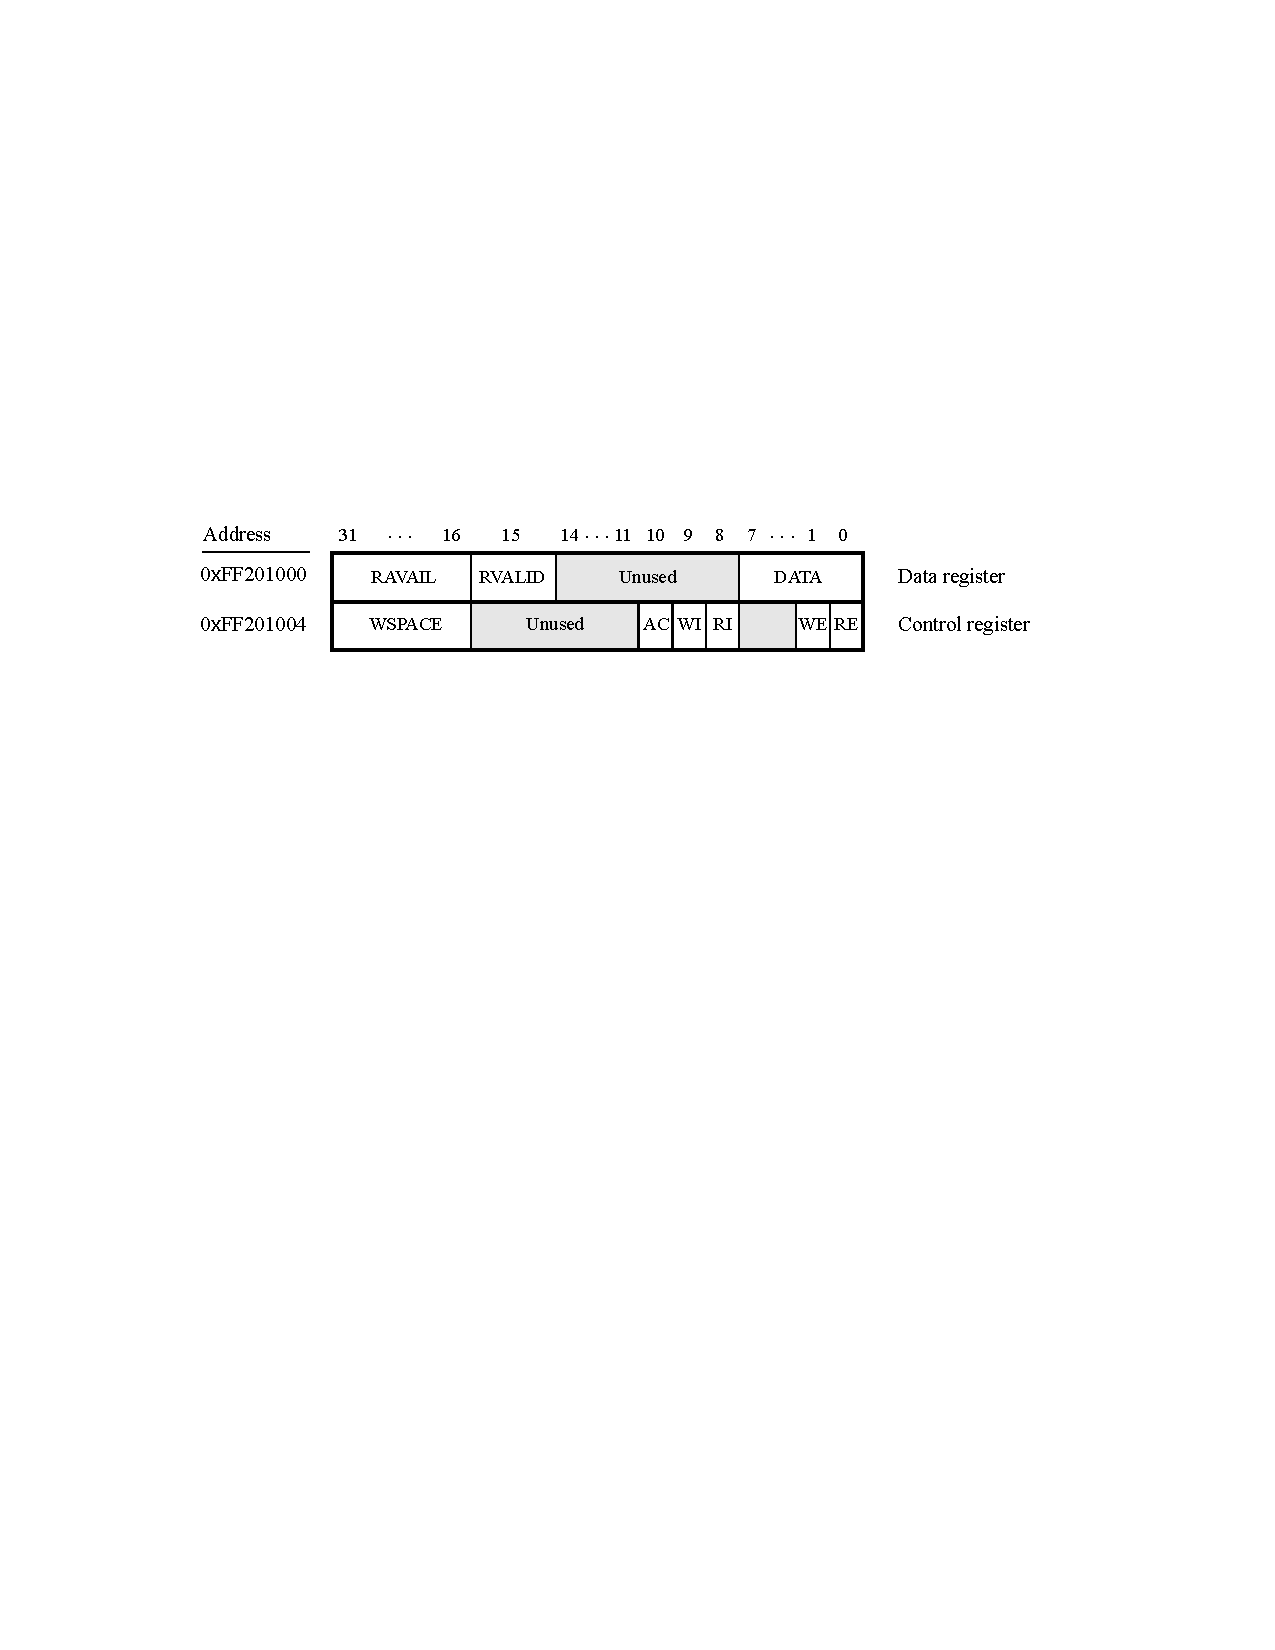
\includegraphics{../../../common/figs/FPGA_JTAG_UART.pdf}
   \end{center}
   \caption{Interrupt bits in the JTAG UART registers.}
	\label{fig:jtag_port_int}
\end{figure}



\subsection{Interrupts from the FPGA Interval Timer}

Figure \ref{fig:interval_port}, in Section \ref{sec:interval_port}, shows six registers that
are associated with the interval timer. As we said in Section \ref{sec:interval_port}, the
{\it TO}~bit in the {\it Status} register is set to 1 when the timer reaches a count value of 0.
It is possible to generate an interrupt when this occurs, by using the {\it ITO}~bit in 
the {\it Control} register. Setting the {\it ITO}~bit to 1 causes an interrupt request to 
be sent to the \GIC~whenever {\it TO} becomes 1. After an interrupt occurs, it can be cleared 
by writing any value into the {\it Status} register.




\subsection{Using Interrupts with Assembly Language Code}

An example of assembly language code for the \systemName~that uses interrupts is
shown in Listing \ref{lst:interrupt_example_s}. When this code is executed on the \DEBoard~board
it displays a rotating pattern on the LEDs. The pattern's rotation can be toggled through pressing the pushbutton KEYs. Two types
of interrupts are used in the code. The LEDs are controlled by an interrupt
service routine for the interval timer, and another interrupt service routine is used to
handle the pushbutton keys. The speed of the rotation is set in the main
program, by using a counter value in the interval timer that causes an interrupt to occur
every 50 msec.

The reset and exception handlers for the main program in Listing \ref{lst:interrupt_example_s} 
are given in Listing \ref{lst:exception_handler_s}. The reset handler simply jumps to the
{\it \_start} symbol in the main program. The exception handler first checks if the
exception that has occurred is an external interrupt or an internal one. In the case of an
internal exception, such as an illegal instruction opcode or a trap instruction, the
handler simply exits, because it does not handle these cases. For external exceptions, it 
calls either the interval timer interrupt service routine, for a level 0 interrupt, or the
pushbutton key interrupt service routine for level 1. These routines are shown in Listings
\ref{lst:interval_timer_isr_s} and \ref{lst:pushbutton_isr_s}, respectively.



\subsection{Using Interrupts with C Language Code}

An example of C language code for the \systemName~that uses interrupts is
shown in Listing \ref{lst:interrupt_example_C}. This code performs exactly the same
operations as the code described in Listing \ref{lst:interrupt_example_s}. 

To enable interrupts the code in Listing \ref{lst:interrupt_example_C} uses {\it macros} 
that provide access to the Nios II status 
and control registers.  A collection of such macros, which can be used in any C program,
are provided in Listing \ref{lst:macros}. 

The reset and exception handlers for the main program in Listing \ref{lst:interrupt_example_C} 
are given in Listing \ref{lst:exception_handler_C}. 
The function called {\it the\_reset} provides a simple reset mechanism by
performing a branch to the main program. The function named {\it the\_exception} 
represents a general exception handler that can be used with any C program. It includes 
assembly language code to check if the exception is caused by an external interrupt, and, 
if so, calls a C language routine named {\it interrupt\_handler}. This routine can then 
perform whatever action is needed for the specific application. In 
Listing~\ref{lst:exception_handler_C}, the {\it interrupt\_handler} code first 
determines which exception has occurred, by using a macro from Listing~\ref{lst:macros} 
that reads the content of the Nios II interrupt pending register.  The interrupt service 
routine that is invoked for the interval timer is shown in \ref{lst:interval_timer_isr_C}, 
and the interrupt service routine for the pushbutton switches appears in 
Listing~\ref{lst:pushbutton_isr_C}.

The source code files shown in Listing \ref{lst:interrupt_example_s} to
Listing~\ref{lst:pushbutton_isr_C} are distributed as part of the  
\productNameMed{}. The files can be found under the heading {\it sample programs}, 
and are identified by the name {\it Interrupt Example}.





% Section: Media Components
\section{Media Components}
\label{sec:multi}

This section describes the audio in/out, video-out, video-in, PS/2, IrDA*, and ADC ports.

\subsection{Audio In/Out Port}

The {\it \systemNameFull} includes an audio port that is connected to the audio CODEC
(COder/DECoder) chip on the \DEBoard~board. The default setting for the 
sample rate provided by the audio CODEC is 
8K samples/sec.  The audio port provides audio-input capability via the microphone 
jack on the \DEBoard~board, as well as audio output functionality via the line-out jack.  
The audio port includes four FIFOs that are used to hold incoming and outgoing data.
Incoming data is stored in the left- and right-channel {\it Read} FIFOs, and outgoing data
is held in the left- and right-channel {\it Write} FIFOs. All FIFOs have a maximum 
depth of 128 32-bit words.

The audio port's programming interface consists of four 32-bit registers, as illustrated in 
Figure \ref{fig:audio_port}.  The {\it Control} register, which has the address 
{\sf 0xFF203040}, is readable to provide status information and writable to make control
settings. Bit {\it RE} of this register provides an interrupt enable capability for
incoming data. Setting this bit to 1 allows the audio core to generate a \processor~interrupt
when either of the {\it Read} FIFOs are filled 75\% or more. The bit {\it RI} will then be
set to 1 to indicate that the interrupt is pending. The interrupt can be cleared by removing
data from the {\it Read} FIFOs until both are less than 75\% full. 
Bit {\it WE} gives an interrupt enable capability for outgoing data. Setting this bit to 
1 allows the audio core to generate an interrupt when either of the {\it Write} FIFOs are
less that 25\% full. The bit {\it WI} will be set to 1 to indicate that the interrupt 
is pending, and it can be cleared by filling the {\it Write} FIFOs until both 
are more than 25\% full.  The bits {\it CR} and {\it CW} in Figure \ref{fig:audio_port} can 
be set to 1 to clear the {\it Read} and {\it Write} FIFOs, respectively. The clear function 
remains active until the corresponding bit is set back to 0.

\begin{figure}[h!]
   \begin{center}
       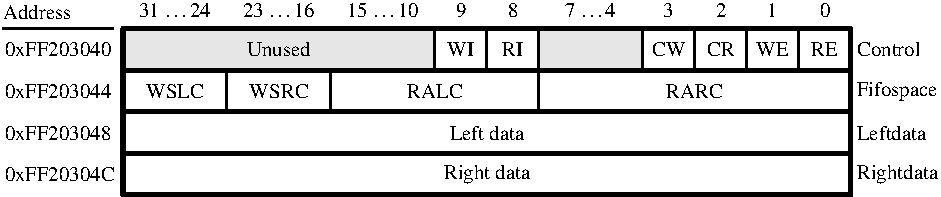
\includegraphics{../../../common/figs/Media_FPGA_Audio_Address_Map.pdf}
   \end{center}
   \caption{Audio port registers.}
	\label{fig:audio_port}
\end{figure}

The read-only {\it Fifospace} register in Figure \ref{fig:audio_port} contains four 8-bit fields.
The fields {\it RARC} and {\it RALC} give the number of words currently stored in the 
right and left audio-input FIFOs, respectively. The fields {\it WSRC} and {\it WSLC} give 
the number of words currently available (that is, {\it unused}) for storing data in the right 
and left audio-out FIFOs. When all FIFOs in the audio port are cleared, the values provided 
in the {\it Fifospace} register are {\it RARC} $=$ {\it RALC} $=$ 0 
and {\it WSRC} $=$ {\it WSLC} $=$ 128.

The {\it Leftdata} and {\it Rightdata} registers are readable for audio in, and writable
for audio out. When data is read from these registers, it is provided from the head of the
{\it Read} FIFOs, and when data is written into these registers it is loaded into the {\it
Write} FIFOs.

A fragment of C code that uses the audio port is shown in Listing \ref{lst:audio_example_C}.
The code checks to
see when the depth of either the left or right {\it Read} FIFO has exceeded 75\% full, and then
moves the data from these FIFOs into a memory buffer. This code is part of a program
that is distributed as part of the \productNameMed{}. The source code can be 
found under the heading {\it sample programs}, and is identified by the name 
{\it Audio}.




\subsection{Video-out Port}
\label{sec:video_out}

The {\it \systemNameFull} includes a video-out port connected to the on-board
\videoOutDevice~controller that can be connected to a standard
\videoOutDevice~monitor. The video-out port support a screen resolution
of 640 $\times$ 480. The image that is displayed by the video-out port is
derived from two sources: a {\it pixel} buffer, and a {\it character} buffer.

\input{\commonPath/Media_FPGA_Pixel_Buffer_\pixelBufferInfo.tex}
\subsubsection{Double Buffering}
\label{sec:double_buffer}

As mentioned above, a pixel buffer controller reads data out of the pixel buffer so that it 
can be displayed on the screen. This pixel buffer controller 
includes a programming interface in the form of a set of registers, as
illustrated in Table~\ref{tab:pixel_ctrl}. The register at address {\sf 0xFF203020} is called 
the {\it Buffer} register, and the register at address  {\sf 0xFF203024} is the 
{\it Backbuffer} register. Each of these registers stores the starting address of a pixel 
buffer.  The Buffer register holds the address of the pixel buffer that is displayed on
the screen. As mentioned above, in the default configuration of the \systemName~this 
Buffer register is set to the address {\sf 0x\baseAddressOffset 8000000}, which points to the start of the FPGA 
on-chip memory.  The default value of the Backbuffer register is also {\sf 0x\baseAddressOffset 8000000},
which means that there is only one pixel buffer. But software can modify the address
stored in the Backbuffer register, thereby creating a second pixel buffer. The pixel
buffer can be located in the SDRAM memory in the \systemName, which has 
the base address {\sf 0x\baseAddressOffset 0000000}. Note that the pixel buffer cannot be located in the DDR3 
memory in the \systemName, because the pixel buffer controller is not connected to 
the DDR3 memory.  An image can be drawn into the second buffer by writing to its pixel addresses.
This image is not displayed on the screen until a pixel buffer {\it swap} is performed, 
as explained below.

A pixel buffer swap is caused by writing the value 1 to the Buffer register. This write
operation does not directly modify the content of the Buffer register, but instead causes
the contents of the Buffer and Backbuffer registers to be swapped. The swap operation does
not happen right away; it occurs at the end of a screen-drawing cycle, after the last 
pixel in the bottom-right corner has been displayed. This time instance is referred to as
the {\it vertical synchronization} time, and occurs every 1/60 seconds. Software can poll the
value of the $S$ bit in the {\it Status} register, at address {\sf 0xFF20302C}, to see when 
the vertical synchronization has happened. Writing the value 1 into the Buffer register
causes $S$ to be set to 1. Then, when the swap of the Buffer and Backbuffer registers 
has been completed $S$ is reset back to 0.  

\begin{table}[h]
    \centering
    \begin{tabular}{|c|l|c|c|c|c|c|c|c|c|c|c|}
        \hline
            \textbf{Address}
            & \multicolumn{1}{c|}{\textbf{Register}}
            & \multirow{2}{*}{\textbf{R/W}}
            & \multicolumn{9}{c|}{\textbf{Bit Description}}
        \\\cline{4-12}
            & \multicolumn{1}{c|}{\textbf{Name}}
            &
            & \textbf{31\ldots24}
            & \textbf{23\ldots16}
            & \textbf{15\ldots12}
            & \textbf{11\ldots8}
            & \textbf{7\ldots6}
            & \textbf{5\ldots3}
            & \textbf{2}
            & \textbf{1}
            & \textbf{0}
        \\\hline
            0xFF203020
            & \texttt{Buffer}
            & R
            & \multicolumn{9}{c|}{Buffer's start address}
        \\\hline
            0xFF203024
            & \texttt{BackBuffer}
            & R/W
            & \multicolumn{9}{c|}{Back buffer's start address}
        \\\hline
            0xFF203028
            & \texttt{Resolution}
            & R
            & \multicolumn{2}{c|}{Y}
            & \multicolumn{7}{c|}{X}
        \\\hline
            \multirow{2}{*}{0xFF20302C}
            & \texttt{Status}
            & R
            & m
            & n
            & {\footnotesize \it (1)}
            & BS
				& SB
            & {\footnotesize \it (1)}
            & EN
            & A
            & S
        \\\cline{2-12}

            & \texttt{Control}
            & W
            & \multicolumn{6}{c|}{\footnotesize \it (1)}
				& EN
            & \multicolumn{2}{c|}{\footnotesize \it (1)}
        \\\hline
                \multicolumn{11}{l}{}
        \\
                \multicolumn{11}{l}{\footnotesize \it{Notes: }}
        \\
                \multicolumn{11}{l}{\footnotesize{(1) Reserved. Read values are undefined. Write zero.}}
    \end{tabular}
		\caption{Pixel Buffer Controller}
		\label{tab:pixel_ctrl}
\end{table}

In a typical application the pixel buffer controller is used as follows. While the image
contained in the pixel buffer that is pointed to by the Buffer register is being displayed, 
a new image is drawn into the pixel buffer pointed to by the Backbuffer register. When this new
image is ready to be displayed, a pixel buffer swap is performed. Then, the pixel buffer 
that is now pointed to by the Backbuffer register, which was already displayed, is cleared and 
the next new image is drawn. In this way, the next image to be displayed is always drawn in
the ``back'' pixel buffer, and the two pixel buffer pointers are swapped when the new image 
is ready to be displayed. Each time a swap is performed software has to synchronize with
the video-out port by waiting until the $S$ bit in the Status register becomes 0.

As shown in Table~\ref{tab:pixel_ctrl} the {\it Status} register contains additional information
other than the $S$ bit. The fields $n$ and $m$ give the number of address bits used for
the $X$ and $Y$ pixel coordinates, respectively. The $BS$ field specifies the number of
data bits per symbol minus one. The $SB$ field specifies the number of symbols per beat minus one. The $A$ field allows 
the selection of two different ways of forming pixel addresses. If configured with $A=0$, then 
the pixel controller expects addresses to contain $X$ and $Y$ fields, as we have used in this
section. But if $A=1$, then the controller expects addresses to be consecutive
values starting from 0 and ending at the total number of pixels$ - 1$. The $EN$ field is used to enable or disable the DMA controller. If this bit is set to 0, the DMA controller will be turned off.

In Table~\ref{tab:pixel_ctrl} the default values of the status register fields in the \systemName~are used when forming pixel addresses. The defaults are $n=9$,  $m=8$,
and $A = 0$. If the pixel buffer controller is changed to provide different values of
these fields, then the way in which pixel addresses are formed has to be modified accordingly. 
The programming interface also includes a {\it Resolution} register, shown 
in Table~\ref{tab:pixel_ctrl}, that contains the X and Y resolution of the pixel buffer(s).  

\subsubsection{Character Buffer}

The character buffer for the video-out port is stored in on-chip memory in the FPGA
on the \DEBoard~board. As illustrated in Figure \ref{fig:chars}$a$, the buffer provides 
a resolution of 80 $\times$ 60 characters, where each character occupies an 8 $\times$ 8
block of pixels on the screen. Characters are stored in each of the locations shown in
Figure \ref{fig:chars}$a$ using their ASCII codes; when these character codes are 
displayed on the monitor, the character buffer automatically generates the
corresponding pattern of pixels for each character using a built-in font. 
Part $b$ of Figure \ref{fig:chars} shows that characters are addressed in the memory by 
using the combination of a {\it base} address, which has the value 
{\sf 0x\baseAddressOffset 9000000}, and an {\it x,y}
offset. Using this scheme, the character at location 0,0 has the address
{\sf 0x\baseAddressOffset 9000000}, 
the character 1,0 has the address {\it base} $+$ (000000 0000001)$_2$ = {\sf 0x\baseAddressOffset 9000001}, 
the character 0,1 has the address {\it base} $+$ (000001 0000000)$_2$ = {\sf 0x\baseAddressOffset 9000080}, and 
the character at location 79,59 has the address {\it base} $+$ (111011 1001111)$_2$ = 
{\sf 0x\baseAddressOffset 9001DCF}. 

\begin{figure}[h!]
   \begin{center}
       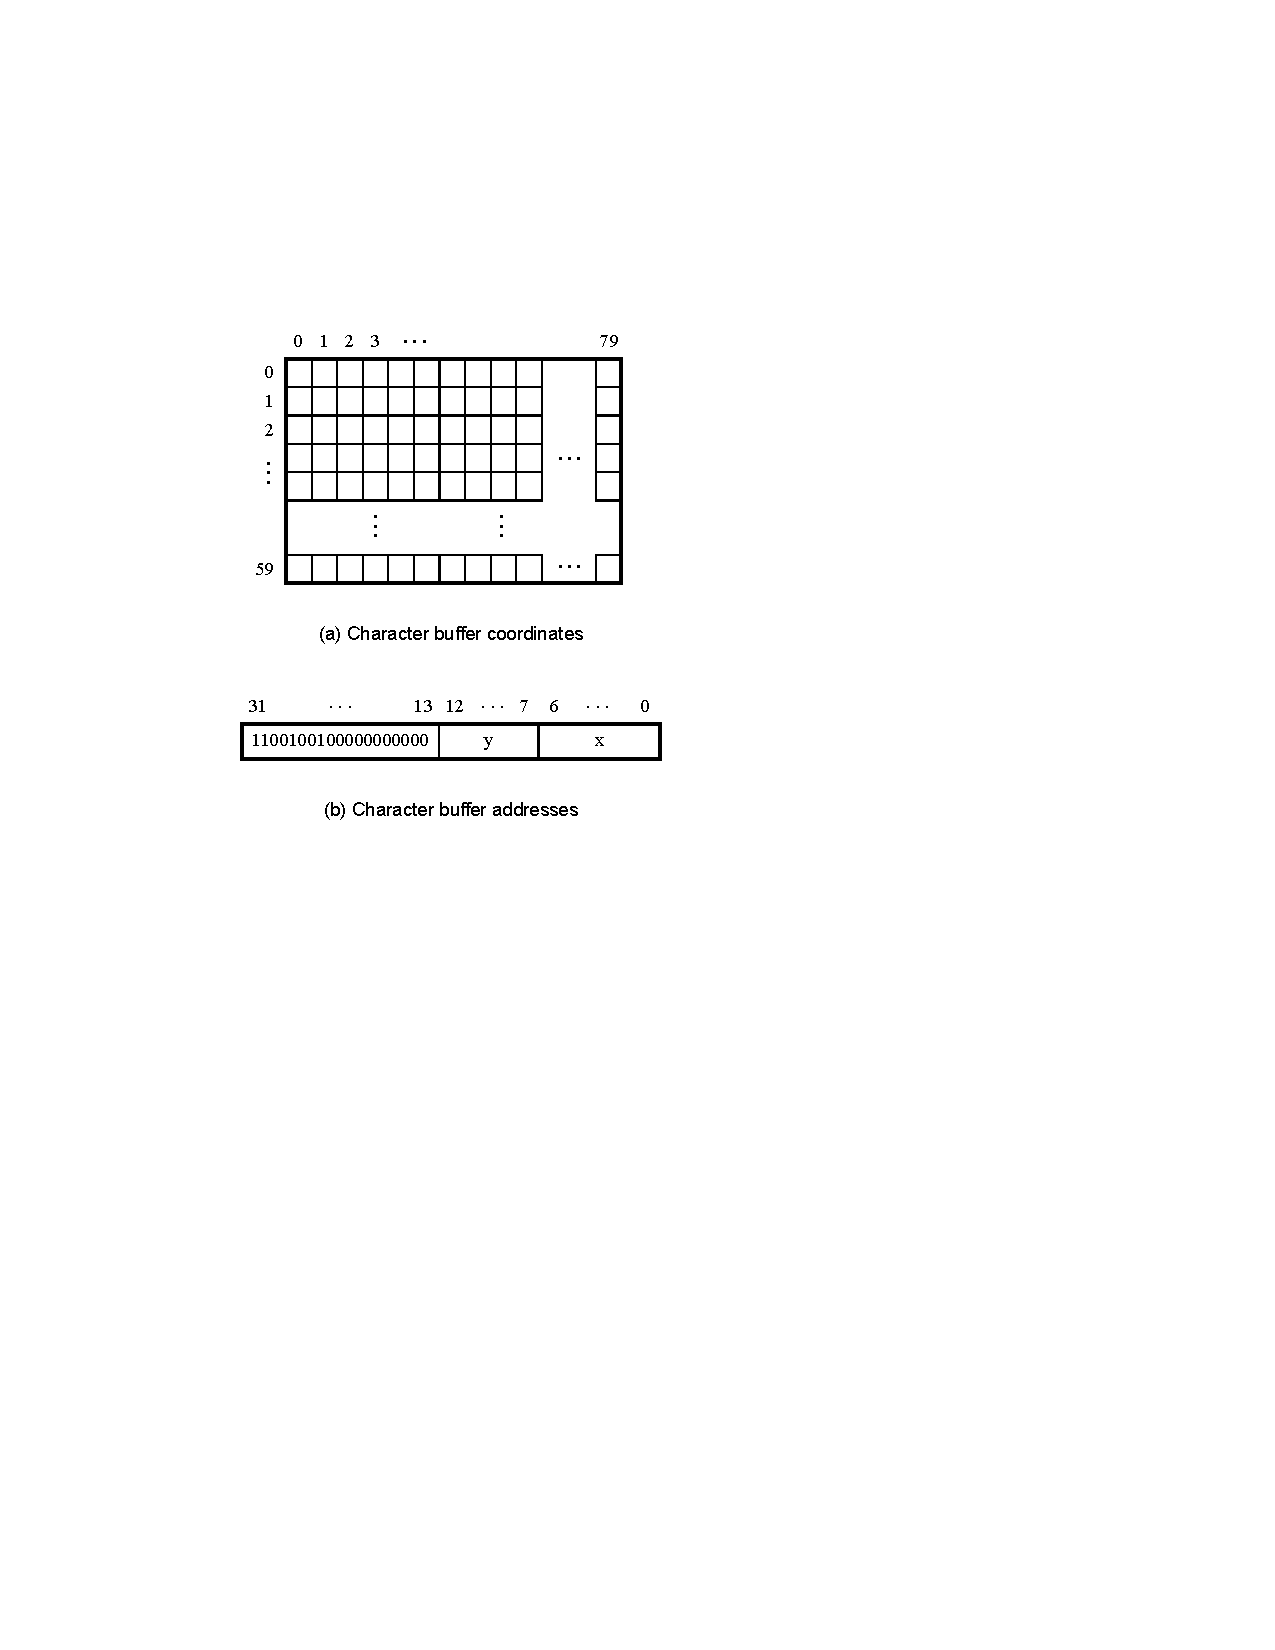
\includegraphics{../../../common/figs/Media_FPGA_Video_Chars.pdf}
   \end{center}
   \caption{Character buffer coordinates and addresses.}
	\label{fig:chars}
\end{figure}

\subsubsection{Using the Video-out Port with C code}

A fragment of C code that uses the pixel and character buffers is shown in 
Listing \ref{lst:video_C}.  The first {\bf for} loop in the figure draws a rectangle in 
the pixel buffer using the color {\it pixel\_color}. The rectangle is drawn using the
coordinates $x_1, y_1$ and $x_2, y_2$.  The second {\bf while} loop in the 
figure writes a null-terminated character
string pointed to by the variable {\it text\_ptr} into the character buffer at the
coordinates {\it x}, {\it y}.  The code in Listing \ref{lst:video_C}
is included in the sample program called {\it Video} that is 
distributed with the \productNameMed{}. 






\subsection{Video-in Port}
\label{sec:video_in}

The {\it \systemNameFull} includes a video-in port for use with the composite video-in
connector on the \DEBoard~board. The video analog-to-digital converter (ADC) connected to this
port is configured to support an NTSC video source. The video-in port provides frames of video 
at a resolution of 320 {\sf x} 240 pixels.  These video frames can be displayed on a 
monitor by using the video-out port described in Section~\ref{sec:video_out}.  The video-in 
port writes each frame of the video-in data into the pixel buffer described in 
Section~\ref{sec:pixel_buffer}. The video-in port can be configured to provide two types
of images: either the ``raw'' image provided by the video ADC, or a version of this image
in which only ``edges'' that are detected in the image are drawn.

The video-in port has a programming interface that consists of two registers, as
illustrated in Figure~\ref{fig:video_in}. The {\it Control} register at the address
{\sf 0xFF20306C} is used to enable or disable the video input. If the {\it EN} bit in this
register is set to 0, then the video-in core does not store any data into the pixel
buffer. Setting {\it EN} to 1 and then changing {\it EN} to 0 can be used to capture a 
still picture from the video-in port.

The register at address {\sf 0xFF203070} is used to enable or disable edge detection.
Setting the {\it E} bit in this register to 1 causes the input video to passed through
hardware circuits that detect edges in the images. The image stored in the pixel buffer
will then consist of dark areas that are punctuated by lighter lines along the edges that
have been detected.  Setting $E=0$ causes a normal image to be stored into the pixel
buffer.

\begin{figure}[h!]
   \begin{center}
       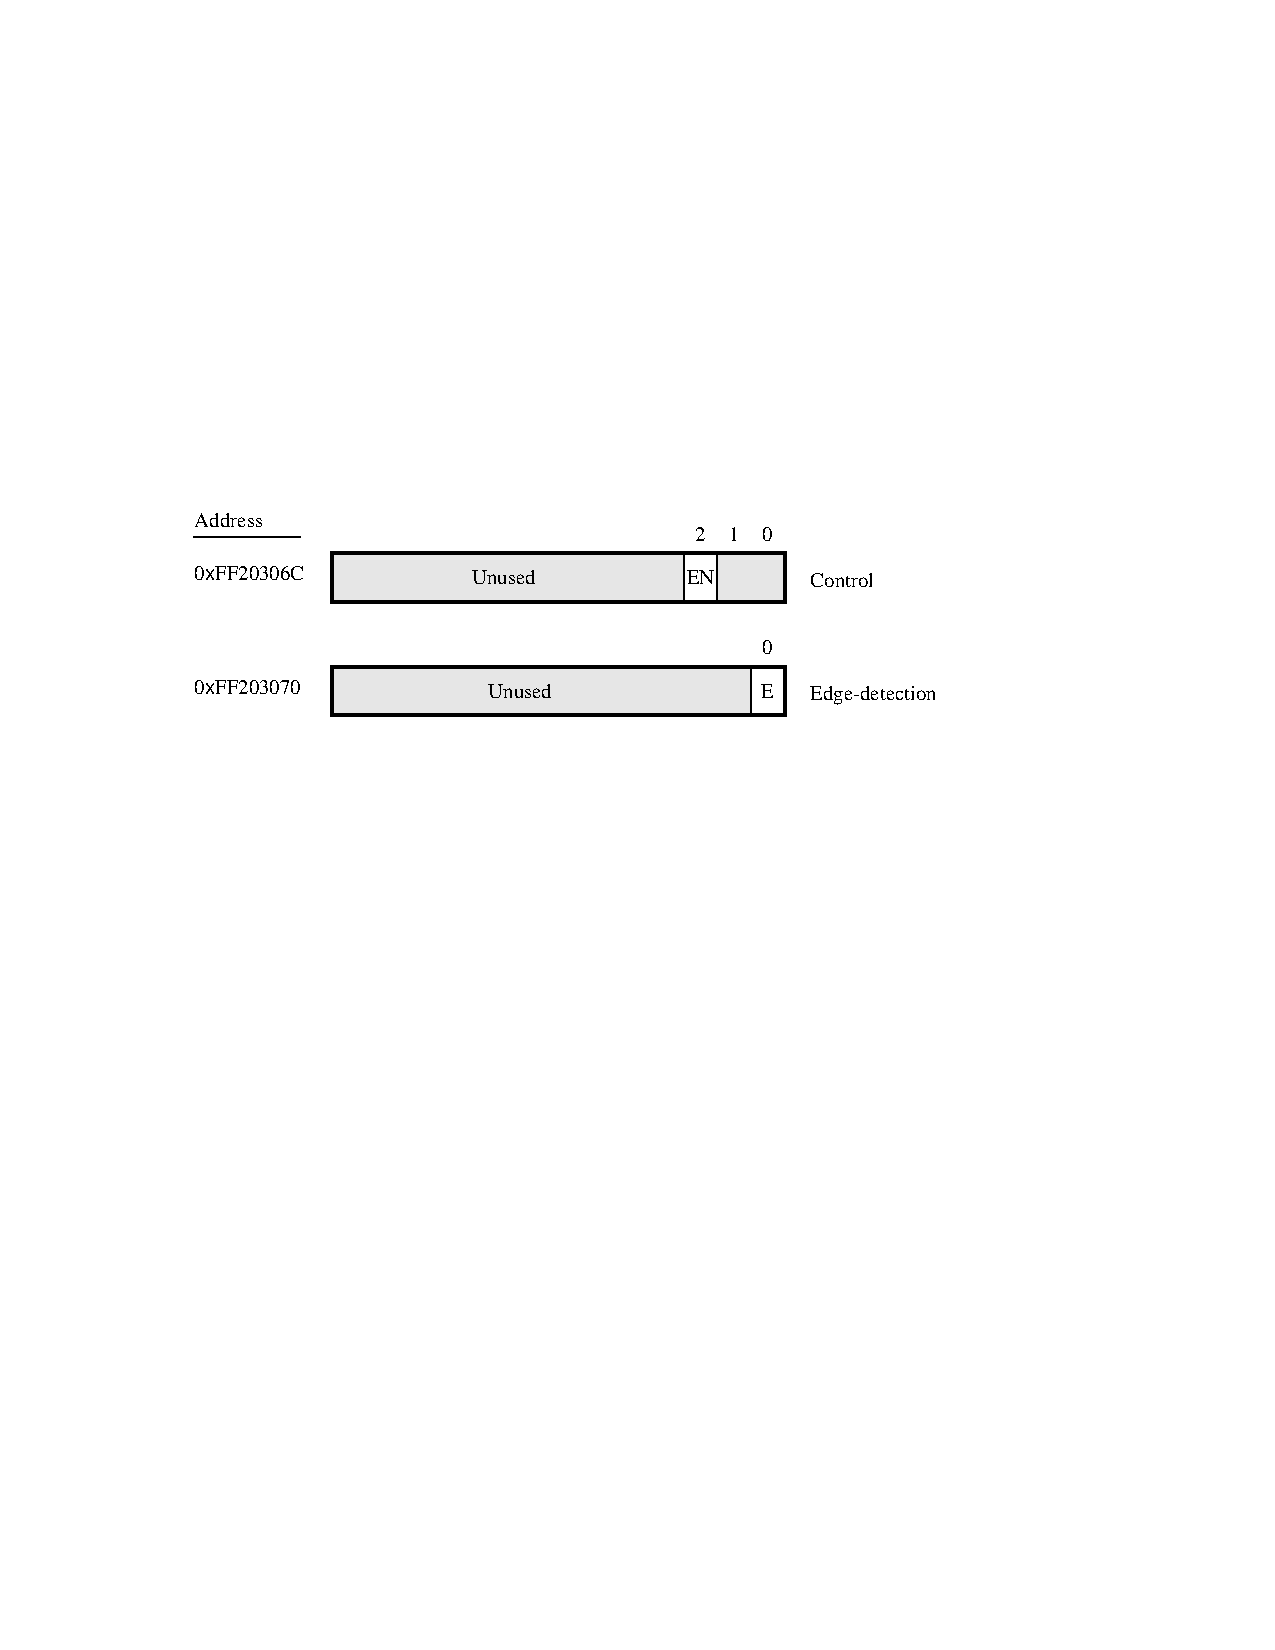
\includegraphics{../../../common/figs/Media_FPGA_Video_In.pdf}
   \end{center}
   \caption{The video-in port programming interface.}
	\label{fig:video_in}
\end{figure}

\subsubsection{DMA Controller for Video}
\label{sec:dma_video}

The data provided by the Video-In core is stored into memory using a DMA Controller for Video. When
operating in {\it Stream to Memory} mode, the DMA stores the incoming frames to memory. 
Table~\ref{tab:video_dma} describes the registers used in the DMA Controller.

\begin{table}[h]
    \centering
    \begin{tabular}{|c|l|c|c|c|c|c|c|c|c|c|c|}
        \hline
            \textbf{Address}
            & \multicolumn{1}{c|}{\textbf{Register}}
            & \multirow{2}{*}{\textbf{R/W}}
            & \multicolumn{9}{c|}{\textbf{Bit Description}}
        \\\cline{4-12}
            & \multicolumn{1}{c|}{\textbf{Name}}
            &
            & \textbf{31\ldots24}
            & \textbf{23\ldots16}
            & \textbf{15\ldots12}
            & \textbf{11\ldots8}
            & \textbf{7\ldots6}
            & \textbf{5\ldots3}
            & \textbf{2}
            & \textbf{1}
            & \textbf{0}
        \\\hline
            0xFF203060
            & \texttt{Buffer}
            & R
            & \multicolumn{9}{c|}{Buffer's start address}
        \\\hline
            0xFF203064
            & \texttt{BackBuffer}
            & R/W
            & \multicolumn{9}{c|}{Back buffer's start address}
        \\\hline
            0xFF203068
            & \texttt{Resolution}
            & R
            & \multicolumn{2}{c|}{Y}
            & \multicolumn{7}{c|}{X}
        \\\hline
            \multirow{2}{*}{0xFF20306C}
            & \texttt{Status}
            & R
            & m
            & n
            & {\footnotesize \it (1)}
            & BS
				& SB
            & {\footnotesize \it (1)}
            & EN
            & A
            & S
        \\\cline{2-12}

            & \texttt{Control}
            & W
            & \multicolumn{6}{c|}{\footnotesize \it (1)}
				& EN
            & \multicolumn{2}{c|}{\footnotesize \it (1)}
        \\\hline
                \multicolumn{11}{l}{}
        \\
                \multicolumn{11}{l}{\footnotesize \it{Notes: }}
        \\
                \multicolumn{11}{l}{\footnotesize{(1) Reserved. Read values are undefined. Write zero.}}
    \end{tabular}
		\caption{Video DMA Controller}
		\label{tab:video_dma}
\end{table}

The incoming video is stored to memory, starting at the address specified in the {\it Buffer} register. The 
{\it BackBuffer} register is used to store an alternate memory location. To change where the video is stored, 
the new location should first be written into the {\it BackBuffer}. Then the value in the {\it BackBuffer} and
{\it Buffer} registers can be switched by performing a write to the {\it Buffer} register. 

Bit 2 of the {\it Status/Control} register, {\it EN}, is used to enable or disable the Video DMA controller.
In the \systemName, the DMA controller is disabled by default. To enable the DMA controller, write a 
1 into this location. The Video DMA Controller will then begin storing the video into the location specified 
in the {\it Buffer} register.

The default value stored in the {\it Buffer} register is {\sf 0x08000000}. This address is also used as the 
source for the Video-Out port, as described in Section~\ref{sec:video_out}, allowing the Video In stream to be 
displayed on the VGA. If the Video-Out is intended to display a different signal, than the address stored in 
the Video DMA Controller's {\it Buffer} register should be changed. 

\subsection{Audio/Video Configuration Module}

The audio/video configuration module controls settings that affect the operation
of both the audio port and the video-out port. The audio/video configuration module
automatically configures and initializes both of these ports whenever the
{\it \systemNameFull} is reset. For typical use of the {\it \systemNameFull} it is not necessary
to modify any of these default settings. 



\subsection{PS/2 Port}

The {\it \systemNameFull} includes two PS/2 ports that can be connected to a standard PS/2
keyboard or mouse. The port includes a 256-byte FIFO that stores data received from a PS/2
device.  The programming interface for the PS/2 port consists of two registers, 
as illustrated in Figure \ref{fig:PS2_port}. The {\it PS2\_Data} register is both readable
and writable. When bit 15, {\it RVALID}, is 1, reading from this register provides the data 
at the head of the FIFO in the
{\it Data} field, and the number of entries in the FIFO (including this read) in the 
{\it RAVAIL} field. When {\it RVALID} is 1, reading from the {\it PS2\_Data} register
decrements this field by 1. Writing to the {\it PS2\_Data} register can be used to send a
command in the {\it Data} field to the PS/2 device.

The {\it PS2\_Control} register can be used to enable interrupts from the PS/2 port by
setting the {\it RE} field to the value 1. When this field is set, then the PS/2 port
generates an interrupt when {\it RAVAIL} $>$ 0. While the interrupt is pending the
field {\it RI} will be set to 1, and it can be cleared by emptying the PS/2 port FIFO. The
{\it CE} field in the {\it PS2\_Control} register is used to indicate that an error
occurred when sending a command to a PS/2 device.

\begin{figure}[h!]
   \begin{center}
       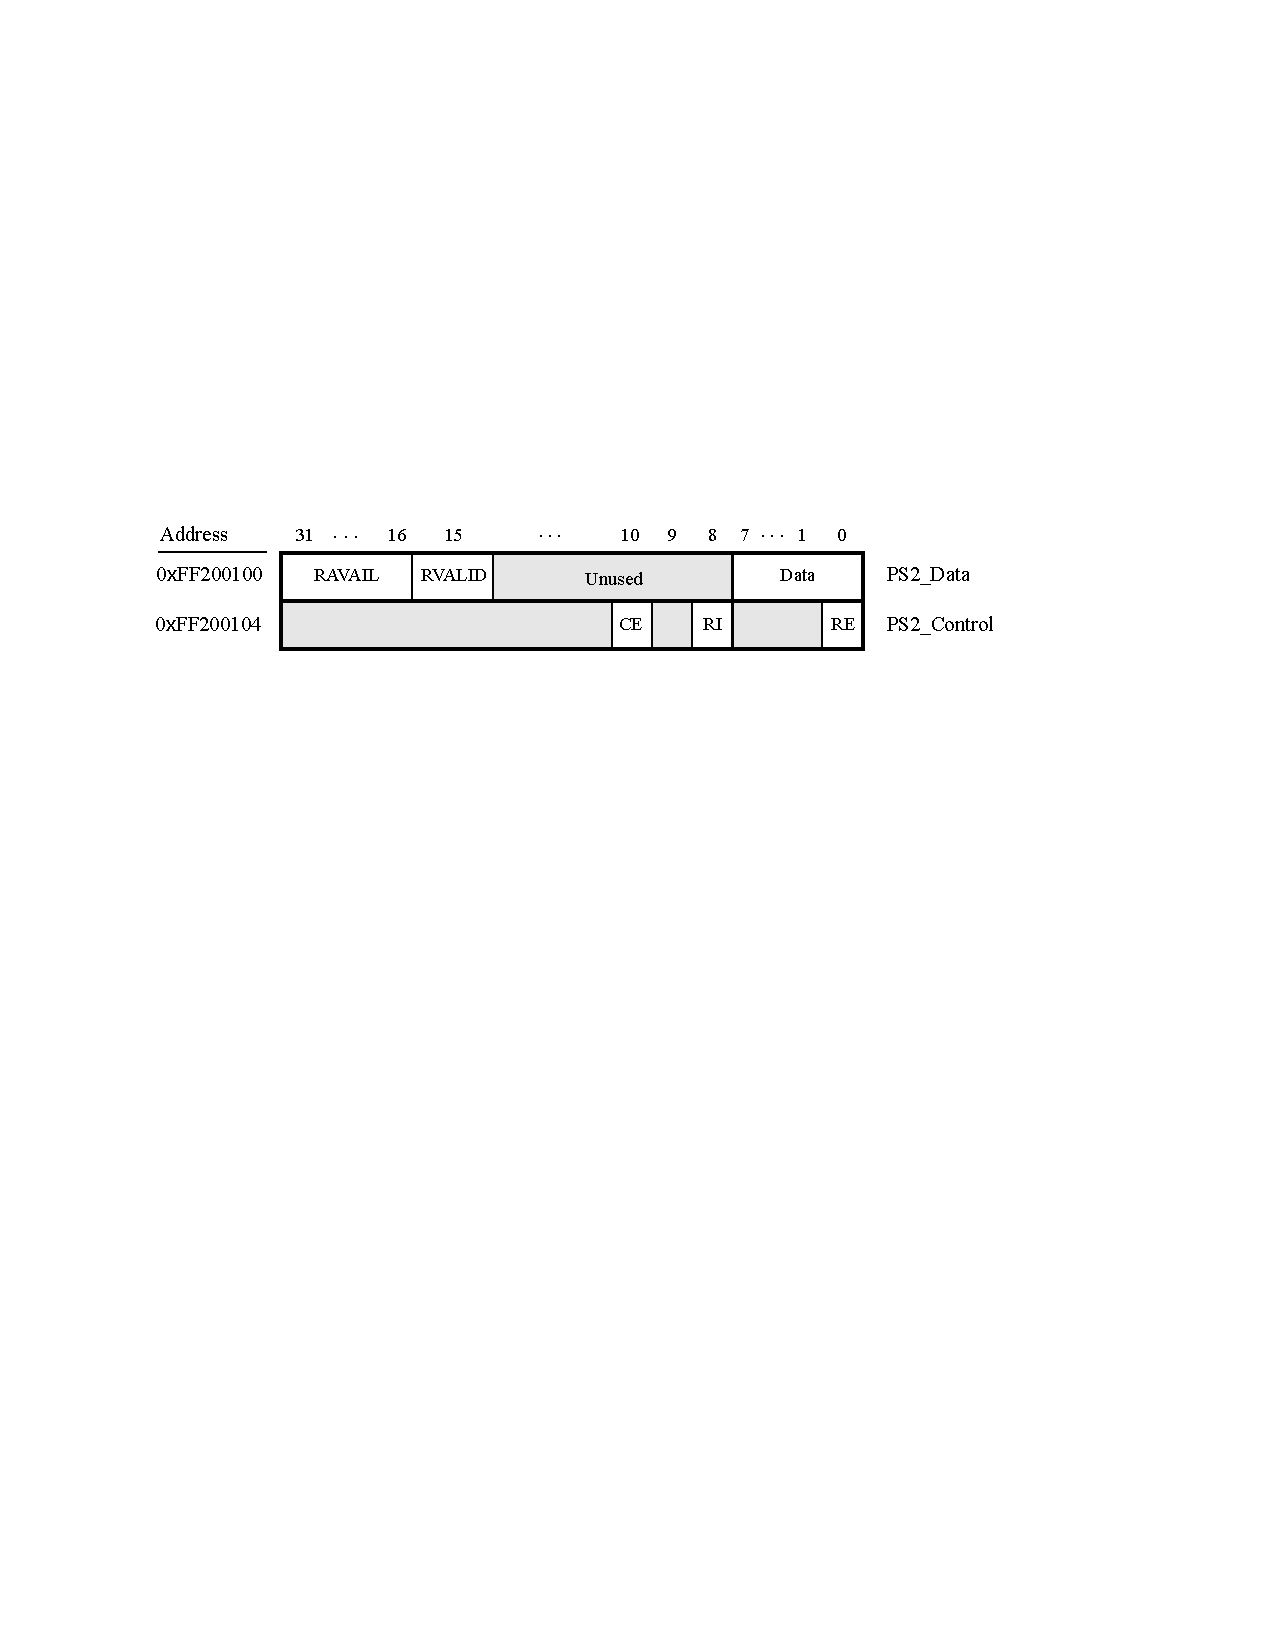
\includegraphics{../../../common/figs/Media_FPGA_PS2.pdf}
   \end{center}
   \caption{PS/2 port registers.}
	\label{fig:PS2_port}
\end{figure}

A fragment of C code that uses the PS/2 port is given in Listing \ref{lst:PS2_C}.  
This code reads the content of the {\it Data} register, and saves data when it is
available.  If the code is used continually in a loop, then it
stores the last three bytes of data received from the
PS/2 port in the variables {\it byte}$_1$, {\it byte}$_2$, and {\it byte}$_3$.
This code is included as part of a sample program
called {\it PS2} that is distributed with the \productNameMed{}. 

\subsubsection{PS/2 Port Dual}

A second PS/2 port is included that allows both a keyboard and mouse
to be used at the same time. To use the dual port a Y-splitter cable must be used and the
keyboard and mouse must be connected to the PS/2 connector on the \DEBoard~board through this
cable. The PS/2 port dual has the same registers as the PS/2 port shown in
Listing~\ref{lst:PS2_C}, except that the base address of its {\it PS2\_Data} register 
is {\sf 0xFF200108} and the base address of its {\it PS2\_Control} register is {\sf 0xFF20010C}.


\subsection{IrDA* Infrared Serial Port}

\label{sec:serial_port}

The IrDA port in the {\it \systemNameFull} implements a UART that is connected to the infrared
transmit/receive device on the \DEBoard~board.
This UART is configured for 8-bit data, one stop bit, and no parity, and
operates at a baud rate of 115,200.  The serial port's programming interface 
consists of two 32-bit registers, as illustrated in Figure~\ref{fig:serial_port}. 
The register at address {\sf 0xFF201020} is referred to as the
{\it Data} register, and the register at address {\sf 0xFF201024} is called the {\it
Control} register.

\begin{figure}[h!]
   \begin{center}
       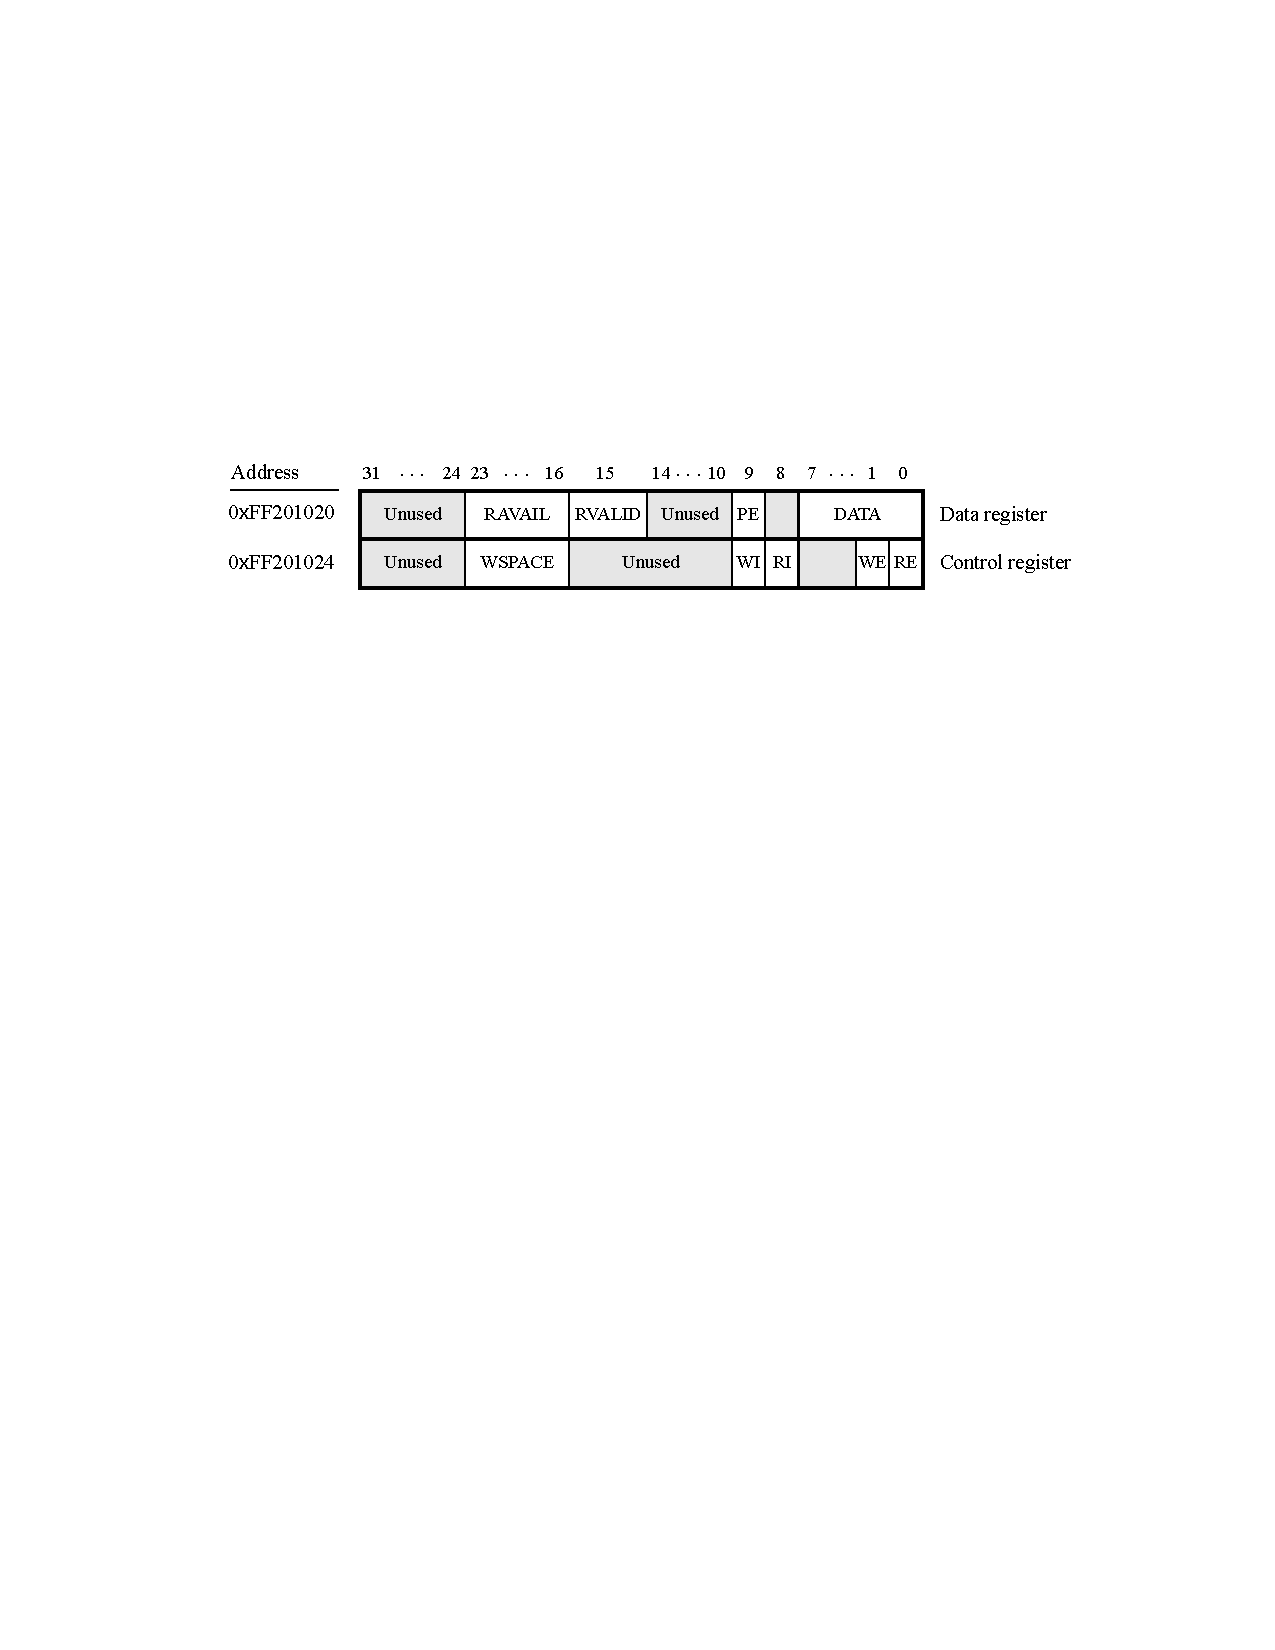
\includegraphics{../../../common/figs/Media_FPGA_IrDA.pdf}
   \end{center}
   \caption{IrDA serial port UART registers.}
	\label{fig:serial_port}
\end{figure}

When character data is received from the IrDA chip it is stored in a 256-character
FIFO in the UART. As illustrated in Figure~\ref{fig:serial_port}, the number 
of characters {\it RAVAIL} currently stored in this FIFO is
provided in bits 23$-$16 of the {\it Data} register.  If the receive FIFO overflows, then
additional data is lost.  When the data that is present in the receive FIFO is available 
for reading, then the value of bit 15, {\it RVALID}, will be 1. Reading the character at
the head of the FIFO, which is provided in bits $7-0$, decrements the value of {\it RAVAIL} 
by one and returns this decremented value as part of the read
operation. If no data is available to be read from the receive FIFO, then {\it RVALID} will 
be set to 0 and the data in bits $7-0$ is undefined.

The UART	also includes a 256-character FIFO that stores data waiting to be sent to the
IrDA device.  Character data is loaded into this register by performing a write to bits 7$-$0
of the {\it Data} register.  Writing into this register has no effect 
on received data.  The amount of space {\it WSPACE} currently available in the transmit FIFO is 
provided in bits 23$-$16 of the {\it Control} register, as indicated 
in Figure~\ref{fig:serial_port}.  If
the transmit FIFO is full, then any additional characters written to the {\it Data} 
register will be lost.

The {\it RE} and {\it WE} bits in the {\it Control} register are used to 
enable \processor~processor interrupts associated with the receive and transmit FIFOs. When enabled, 
interrupts are generated when {\it RAVAIL} for the receive FIFO, or {\it WSPACE} for
the transmit FIFO, exceeds 31. Pending interrupts are indicated in the {\it Control}
register's {\it RI} and {\it WI} bits, and can be cleared by writing or reading data
to/from the UART.



\subsection{Analog-to-Digital Conversion Port}

\label{sec:ADC_port}

The Analog-to-Digital Conversion (ADC) Port provides access to the eight-channel, 12-bit
analog-to-digital converter on the \DEBoard~board. As illustrated in
Figure~\ref{fig:ADC_port}, the ADC port comprises eight 12-bit registers starting at the
base address {\sf 0xFF204000}. The first two registers have dual purposes, acting as both
data and control registers.  By default, the ADC port updates the A-to-D conversion
results for all ports only when instructed to do so. Writing to the control register at 
address {\sf 0xFF204000} causes this update to occur. Reading from the register at address
{\sf 0xFF204000} provides the conversion data for channel 0. Reading from the other seven
registers provides the conversion data for the corresponding channels. It is also
possible to have the ADC port continually request A-to-D conversion data for all channels.
This is done by writing the value 1 to the control register at address {\sf 0xFF204004}.
The {\it R} bit of each channel register in Figure~\ref{fig:ADC_port} is used in Auto-update mode.
{\it R} is set to 1 when its corresponding channel is refreshed and set to 0 when the channel is read.

\begin{figure}[h!]
   \begin{center}
       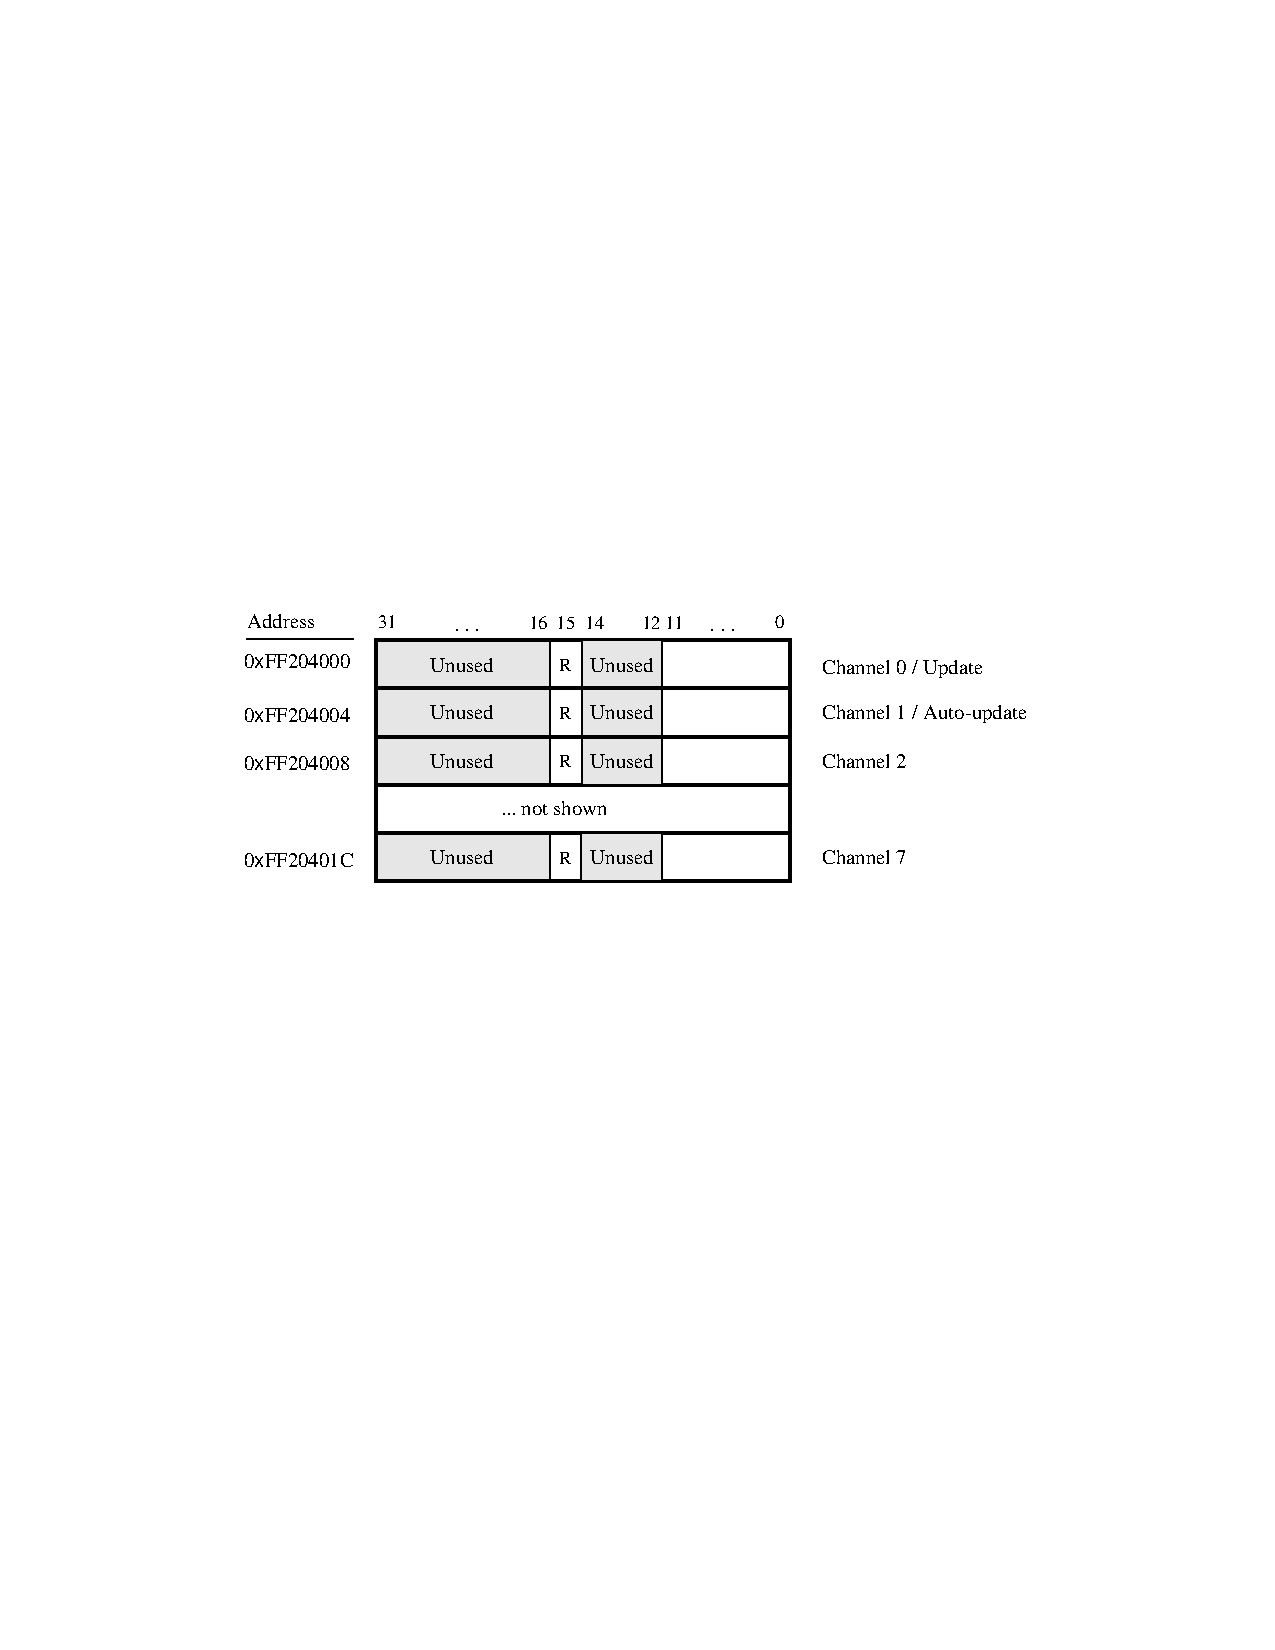
\includegraphics{../../../common/figs/Media_FPGA_ADC.pdf}
   \end{center}
   \caption{ADC port registers.}
	\label{fig:ADC_port}
\end{figure}

Figure~\ref{fig:ADC_conn} shows the connector on the \DEBoard~board that is used with the
ADC port. Analog signals in the range of 0 V to the $V_{CC5}$ power-supply voltage can be 
connected to the pins for channels 0 to 7. 

\begin{figure}[h!]
   \begin{center}
       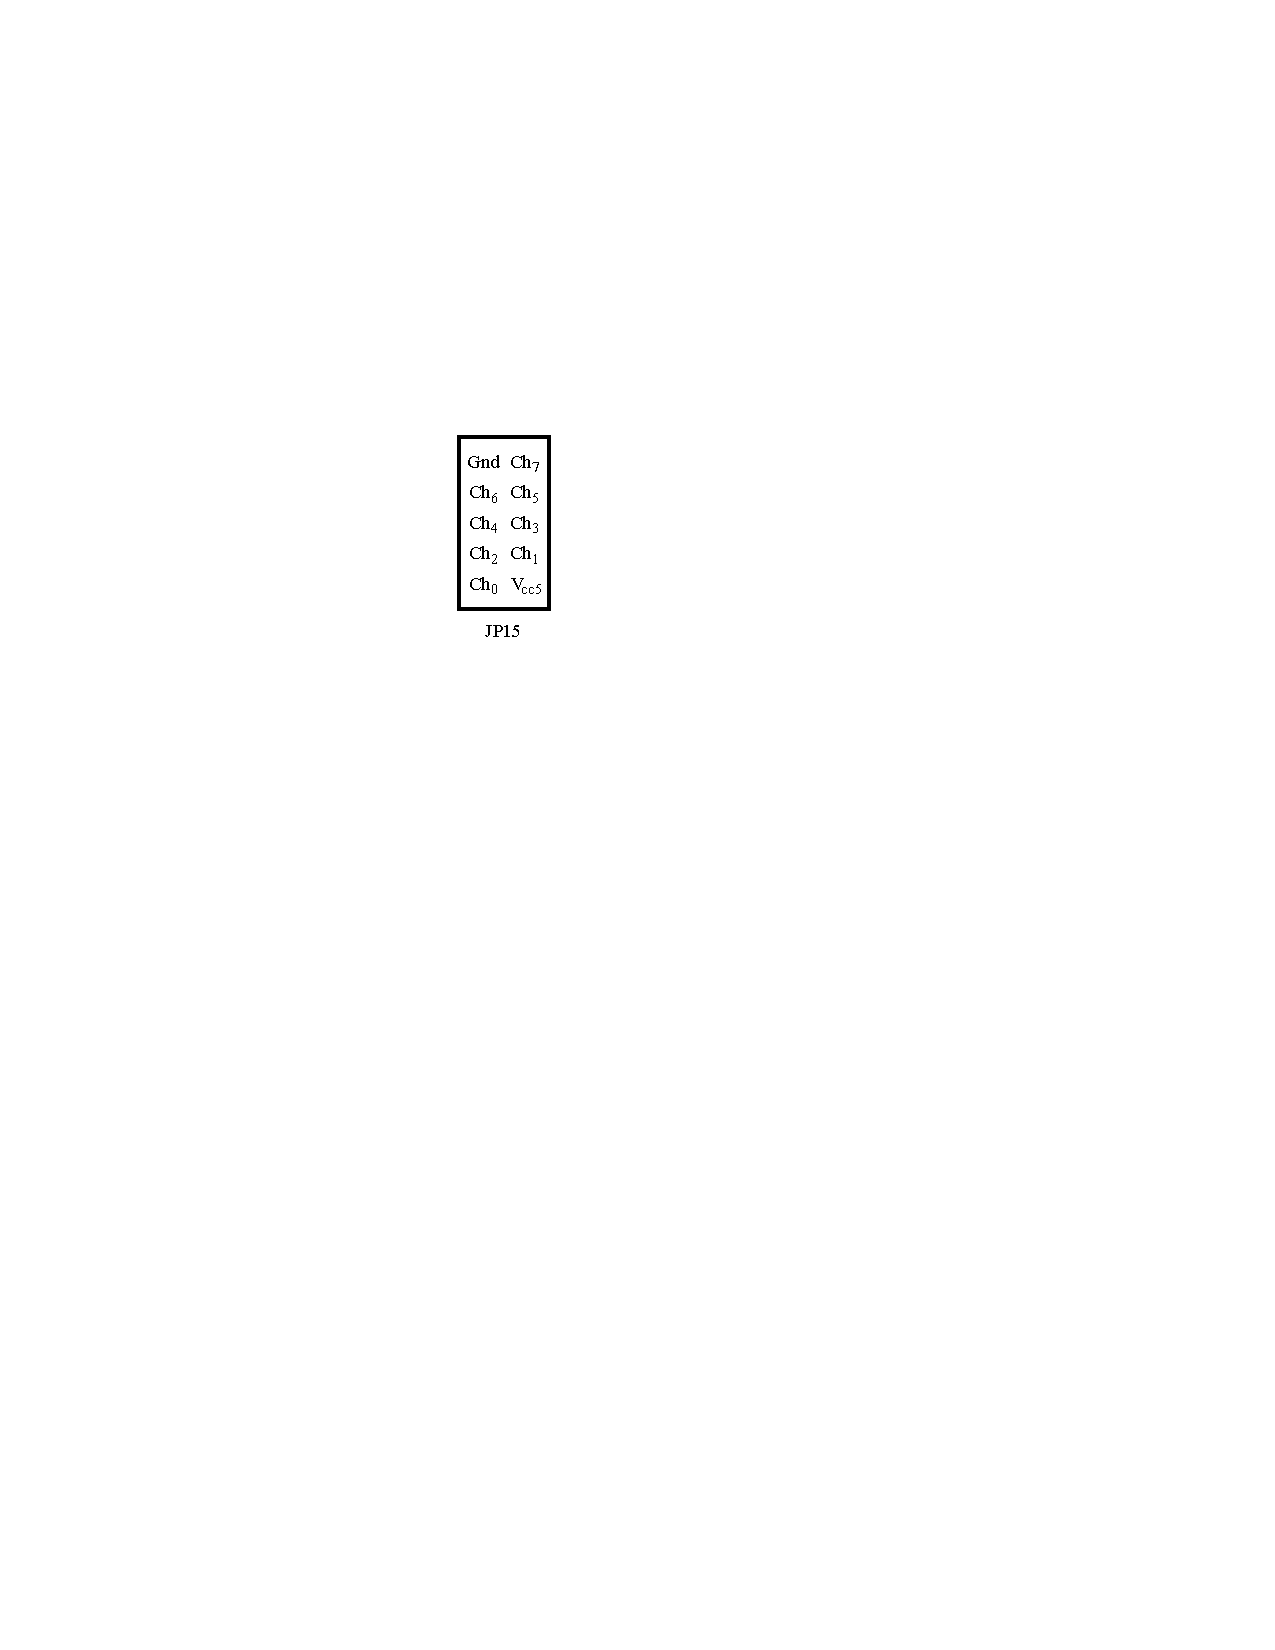
\includegraphics{../../../common/figs/Media_FPGA_ADC_Conn.pdf}
   \end{center}
   \caption{ADC connector.}
	\label{fig:ADC_conn}
\end{figure}




% Section: Modifying the System
\section{Modifying the \systemNameFull}

It is possible to modify the {\it \systemNameFull} 
by using the Quartus\textsuperscript{\textregistered} Prime software
and {\systemBuilder} tool. Instructions for using this software are
provided as part of the
\texttt{Computer Organization and System Design} tutorials on the 
{\small \href{https://www.fpgacademy.org/tutorials.html} {FPGAcademy.org}} website.
To modify the system it is first necessary to make an editable copy of the 
{\it \systemNameFull}. The files for this system are installed as part of the Monitor 
Program installation. Locate these files, copy them to a working directory, and then 
use the Quartus Prime and {\systemBuilder} software to make any desired changes.

Table \ref{tab:sopcnames} lists the names of the {\systemBuilder} IP cores that are used 
in this system. When the {\it \systemNameFull} design files are opened in the Quartus 
Prime software, these cores can be examined using the {\systemBuilder} System Integration 
tool.  Each core has a number of settings that are selectable in the {\systemBuilder} 
System Integration tool, and includes a datasheet that provides detailed documentation.

The steps needed to modify the system are:

\begin{enumerate}
\item Make of copy of the design source files for the {\it \systemNameFull} from the its 
GitHub repository. 
\item Open the top-level project file (*.{\it qpf}) in the Quartus Prime software
\item Open the {\systemBuilder} System Integration tool in the Quartus Prime software, and 
modify the system as desired
\item Generate the modified system by using the {\systemBuilder} System Integration tool
\item It may be necessary to modify the Verilog code in the top-level module of the project, 
if any I/O peripherals have been added or removed from the system
\item Compile the project in the Quartus Prime software
\item Download the modified system into the \DEBoard~board
\end{enumerate}

Note: to compile and use a new version of the {\it \systemNameFull} it may be necessary to
request a license from Altera that allows you to create circuit that includes 
the {\processor} processor.


\begin{table}[h]
    \begin{center}
    \begin{tabular}{l|l}
            \textbf{I/O Peripheral}
            & \textbf{Qsys Core}
        \\\hline
            SDRAM
            & SDRAM Controller
        \\
            SRAM
        &   SRAM Controller
        \\
            On-chip memory character buffer
				& Character Buffer for VGA Display
        \\
            SD Card
        &   SD Card Interface
        \\
            Flash
        &   Flash Memory IP Core
        \\
            Red LED parallel port
				& Parallel Port
        \\
            7-segment displays parallel port
				& Parallel Port
        \\
            Expansion parallel ports
				& Parallel Port
        \\
            Slider switch parallel port
				& Parallel Port
        \\
            Pushbutton parallel port
				& Parallel Port
        \\
            PS/2 port
				& PS2 Controller
        \\
            JTAG port
				& JTAG UART
        \\
            Serial port
				& RS232 UART
        \\
            IrDA port
				& IrDA UART
        \\
            Interval timer
				& Interval timer 
        \\
            System ID
				& System ID Peripheral
        \\
            Audio/video configuration port
				& Audio and Video Config
        \\
            Audio port
				& Audio
        \\
            Video port
				& Pixel Buffer DMA Controller
        \\
            Video In port
				& DMA Controller
        \\
    \end{tabular}
    \caption{Qsys cores used in the \systemName.}
    \label{tab:sopcnames}
    \end{center}
\end{table}
\clearpage

% Section: Making the System the Default Configuration
\section{Making the System the Default Configuration}
\label{sec:systempof}

The {\it \systemNameFull} can be loaded into the nonvolatile FPGA configuration memory on the
\DEBoard~board, so that it becomes the default system whenever the board is powered on.
Instructions for configuring the \DEBoard~board in this manner can be found in the tutorial
{\it Introduction to the Quartus Prime Software}, which is available as part of the
\texttt{Digital Logic Hardware Design} tutorials in the 
{\small \href{https://www.fpgacademy.org/tutorials.html} {FPGAcademy.org}} website.




\section{Memory Layout}

\noindent
Table \ref{tab:memorylayout} summarizes the memory map used in the \systemName.
~\\
~\\

\begin{table}[h]
    \begin{center}
    \begin{tabular}{c|c|l}
            \textbf{Base Address}
            & \textbf{End Address}
            & \textbf{I/O Peripheral}
				\\\hline\vspace{-3mm}\\
            0x00000000
            & 0x03FFFFFF
            & SDRAM
        \\
            0x08000000
            & 0x0803FFFF
            & FPGA On-chip Memory
        \\
            0x09000000
            & 0x09001FFF
            & FPGA On-chip Memory Character Buffer
        \\
            0x40000000
            & 0x7FFFFFFF
            & DDR3 Memory
        \\
            0xFF200000
            & 0xFF20000F
            & Red LEDs
        \\
            0xFF200020
            & 0xFF20002F
            & 7-segment HEX3$-$HEX0 Displays
        \\
            0xFF200030
            & 0xFF20003F
            & 7-segment HEX5$-$HEX4 Displays

        \\
            0xFF200040
            & 0xFF20004F
            & Slider Switches
        \\
            0xFF200050
            & 0xFF20005F
            & Pushbutton KEYs
        \\
            0xFF200060
            & 0xFF20006F
            & JP1 Expansion
        \\
            0xFF200070
            & 0xFF20007F
            & JP2 Expansion
        \\
            0xFF200100
            & 0xFF200107
            & PS/2
        \\
            0xFF200108
            & 0xFF20010F
            & PS/2 Dual
        \\
            0xFF201000
            & 0xFF201007
            & JTAG UART
        \\
            0xFF201020
            & 0xFF201027
				& Infrared (IrDA)
        \\
            0xFF202000
            & 0xFF20201F
            & Interval Timer
        \\
            0xFF202020
            & 0xFF20202F
            & Second Interval Timer
        \\
            0xFF203000
            & 0xFF20301F
            & Audio/video Configuration
        \\
            0xFF203020
            & 0xFF20302F
            & Pixel Buffer Control
        \\
            0xFF203030
            & 0xFF203037
            & Character Buffer Control
        \\
            0xFF203040
            & 0xFF20304F
            & Audio
        \\
            0xFF203060
            & 0xFF203070
            & Video-in
        \\
            0xFF204000
            & 0xFF20401F
            & ADC
        \\
            0xFFC04000
            & 0xFFC040FC
            & HPS I2C0
        \\
    \end{tabular}
    \caption{Memory layout used in the \systemName.}
    \label{tab:memorylayout}
    \end{center}
\end{table}

% Section: AMP Integration
\newpage
\section{\productNameMed{} Integration} 
\label{sec:monitor_program}

As we mentioned earlier, the {\it \systemNameFull} system, and the sample programs described
in this document, are made available as part of the \productNameMed{}. Figures
\ref{fig:monitor_project} to
\ref{fig:monitor_last} show a series of windows that are used in the Monitor 
Program to create a new project.
In the first screen, shown in Figure \ref{fig:monitor_project}, the user specifies a 
file system folder where the
project will be stored, gives the project a name, and specifies the type of processor that
is being used. Pressing {\sf Next} opens the window
in Figure \ref{fig:monitor_system}. Here, the user can select the {\it \systemNameFull} 
as a pre-designed system.
The Monitor Program then fills in the relevant information in the {\it System details} box,
which includes the appropriate system info and FPGA configuration files, and preloader.
The first of these files specifies to the Monitor Program information about the components 
that are available in the {\it \systemNameFull}, such as the type of processor and memory 
components, and the address map. The second file is an FPGA programming bitstream for 
the {\it \systemNameFull}, which can downloaded by the Monitor Program into the \DEBoard~board. 
Any system which contains a Hard Processor System (HPS) component must also specify the preloader to be
run immediately following the circuit being downloaded. This preloader is used to configure the components
within the HPS with the setting required for the specific board.
~\\
~\\
\begin{figure}[h!]
	\centering
	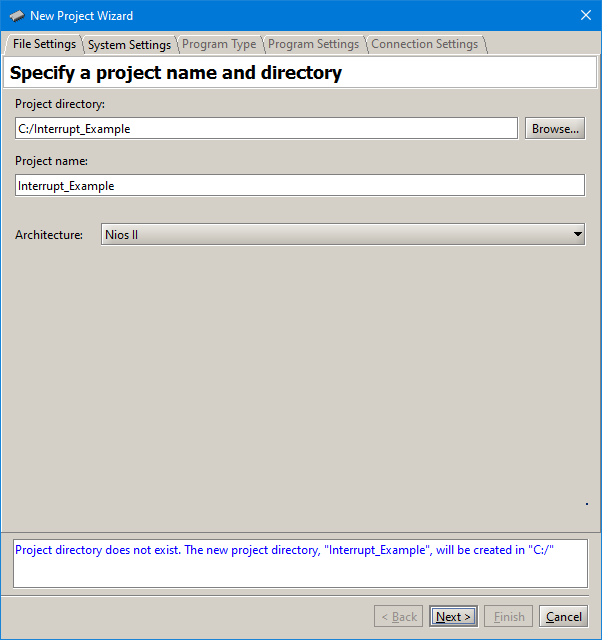
\includegraphics[scale=0.65]{figures/fig_monitor_project.png}
	\caption{Specifying the project folder and project name.}
	\label{fig:monitor_project}
\end{figure}

\clearpage
\newpage
Pressing {\sf Next} again opens the window in Figure \ref{fig:monitor_samples}. Here the
user selects the type of program that will be used, such as Assembly language, or C. Then,
the check box shown in the figure can be used to display the list of sample programs for
the {\it \systemNameFull} that are described in this document. When a sample program
is selected in this list, its source files, and other settings, can be copied into the 
project folder in subsequent screens of the Monitor Program.

Figure \ref{fig:monitor_last} gives the final screen that is 
used to create a new project in the Monitor Program. This screen shows the default addresses of 
compiler and linker sections that will be used for the assembly language or C program 
associated with the Monitor Program project.  In the figure, the drop-down menu called 
{\it Linker Section Presets} has been set to {\sf Exceptions}. With this setting the 
Monitor Program uses specific compiler and linker sections for the selected processor.
For the \processor processor, these sections are for reset and
trap handler, and another section for the main program, called .{\it text}. For the
A9 processor, it has a section for the exception table, 
called .{\it vectors}, and another section
for the main program, called .{\it text}. It also shows the initial value used to set the main 
stack pointer for C programs, which is the starting address of the .{\it stack} section.
~\\
~\\
\begin{figure}[h!]
	\centering
	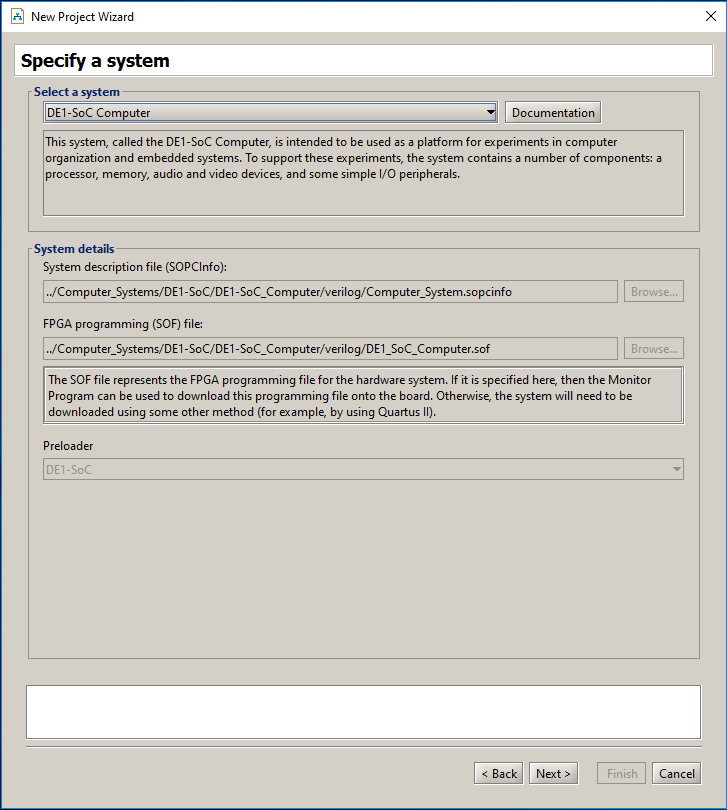
\includegraphics[scale=0.60]{figures/fig_monitor_system.png}
	\caption{Specifying the {\systemNameFull}.}
	\label{fig:monitor_system}
\end{figure}

\begin{figure}[h!]
	\centering
	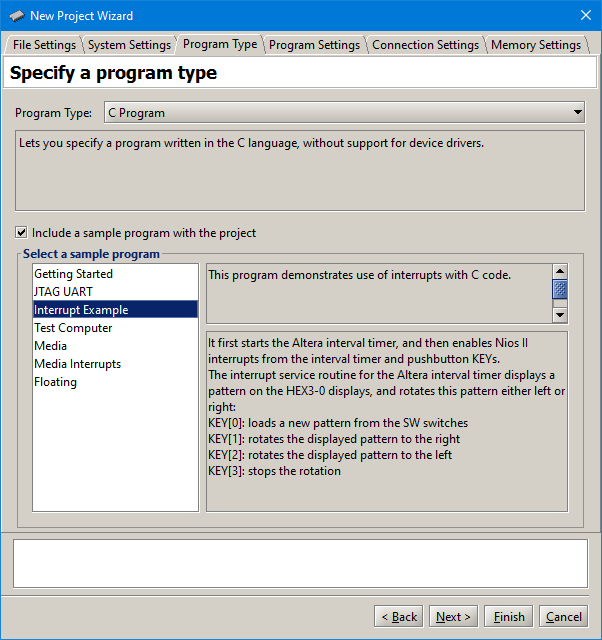
\includegraphics[scale=0.55]{figures/fig_monitor_samples.png}
	\caption{Selecting sample programs.}
	\label{fig:monitor_samples}
\end{figure}

\begin{figure}[h!]
\centering
	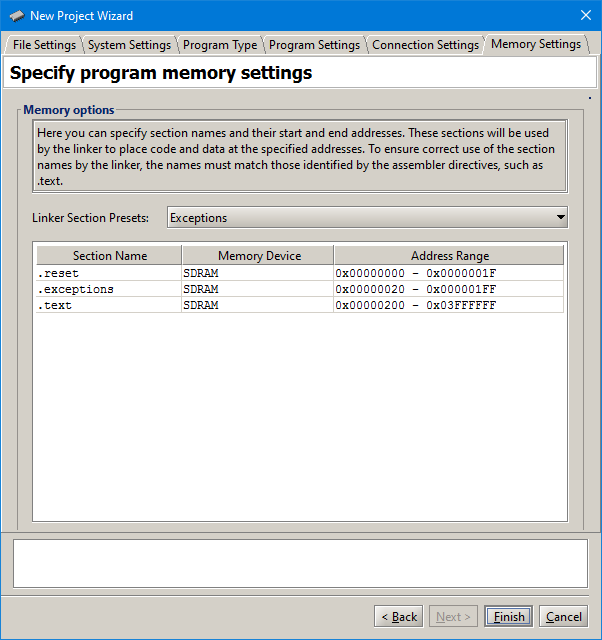
\includegraphics[scale=0.55]{figures/fig_monitor_last.png}
	\caption{Setting offsets for .{\it text} and .{\it data}.}
	\label{fig:monitor_last}
\end{figure}


\clearpage

% Appendix
\input{\commonPath/appendix.tex}
\subsection{Parallel Ports}

\expandparam
\lstinputlisting[style=\processorStyle, caption={An example of \processor~assembly
language code that uses parallel ports.}, captionpos=b, label={lst:getting_started_s},
showlines=true]{\sampleProgramsPath/\processorLower/asm/getting_started/getting_started.s}
\newpage

\lstinputlisting[language=C, caption={An example of C code that uses parallel ports.}, captionpos=b, label={lst:getting_started_C}]{\sampleProgramsPath/\processorLower/c/getting_started/getting_started.c}
\newpage
\subsection{JTAG* UART}

% Assembly Source Code
\expandparam
\lstinputlisting[style=\processorStyle, caption={An example of assembly language code that
uses the JTAG UART (Part $a$).}, captionpos =b, label={lst:jtag_uart_s}, lastline=35,
showlines=true]{\sampleProgramsPath/\processorLower/asm/JTAG_UART/JTAG_UART.s}
\newpage
\expandparam
\lstinputlisting[style=\processorStyle, captionpos=b, firstline=36]{\sampleProgramsPath/\processorLower/asm/JTAG_UART/JTAG_UART.s}
\begin{center}
Listing \ref{lst:jtag_uart_s}. An example of assembly language code that uses the JTAG UART (Part {\it b}).
\end{center}
\newpage

\lstinputlisting[language=C, caption={An example of C code that uses the JTAG UART (Part a).}, captionpos=b, label={lst:jtag_uart_C}]{\sampleProgramsPath/\processorLower/c/JTAG_UART/JTAG_UART.c}
\newpage
\lstinputlisting[language=C, captionpos=b]{\sampleProgramsPath/\processorLower/c/JTAG_UART/main.c}
\begin{center}
Listing \ref{lst:jtag_uart_C}. An example of C code that uses the JTAG UART (Part {\it b}).
\end{center}
\newpage


\subsection{Interrupts}

% Assembly source files

% interrupt example
\lstinputlisting[style=defaultNiosStyle, caption={An example of assembly language code that uses interrupts.}, captionpos=b, label={lst:interrupt_example_s}]{\sampleProgramsPath/nios2/asm/interrupt_example/interrupt_example.s}
\newpage

% exception handlers
\lstinputlisting[style=defaultNiosStyle, caption={Reset and exception handler assembly language code.}, captionpos=b, label={lst:exception_handler_s}]{\sampleProgramsPath/nios2/asm/interrupt_example/exception_handler.s}
\newpage

% interval timer interrupt
\lstinputlisting[style=defaultNiosStyle, caption={Interrupt service routine for the interval timer.}, captionpos=b, label={lst:interval_timer_isr_s}]{\sampleProgramsPath/nios2/asm/interrupt_example/interval_timer_isr.s}
\newpage

% key interrupt
\lstinputlisting[style=defaultNiosStyle, caption={Interrupt service routine for the pushbutton KEYs.}, captionpos=b, label={lst:pushbutton_isr_s}]{\sampleProgramsPath/nios2/asm/interrupt_example/pushbutton_isr.s}
\newpage

% C Source Code

% interrupt example
\lstinputlisting[language=C, caption={An example of C code that uses interrupts.}, captionpos=b, label={lst:interrupt_example_C}]{\sampleProgramsPath/nios2/c/interrupt_example/interrupt_example.c}
\newpage

% macros
\lstinputlisting[language=C, caption={Macros for accessing Nios II status and control registers.}, captionpos=b, label={lst:macros}]{\sampleProgramsPath/nios2/c/interrupt_example/nios2_ctrl_reg_macros.h}
\newpage

% Exceptions Handler
\lstinputlisting[language=C, caption={Reset and exception handler C code.}, captionpos=b, label={lst:exception_handler_C}]{\sampleProgramsPath/nios2/c/interrupt_example/exception_handler.c}
\newpage

% interval timer interrupt
\lstinputlisting[language=C, caption={Interrupt service routine for the interval timer.}, captionpos=b, label={lst:interval_timer_isr_C}]{\sampleProgramsPath/nios2/c/interrupt_example/interval_timer_ISR.c}
\newpage

% key interrupt
\lstinputlisting[language=C, caption={Interrupt service routine for the pushbutton KEYs.}, captionpos=b, label={lst:pushbutton_isr_C}]{\sampleProgramsPath/nios2/c/interrupt_example/pushbutton_ISR.c}
\newpage

\subsection{Audio}

\lstinputlisting[language=C, label={lst:audio_example_C}, caption={An example of code that uses the audio port.}, captionpos=b]{\sampleProgramsPath/\processorLower/c/audio/audio.c}
\newpage
\subsection{Video Out}

\lstinputlisting[language=C, label={lst:video_C}, caption={An example of code that uses the video-out port.}, captionpos=b]
{\sampleProgramsPath/\processorLower/c/video/video.c}
\newpage

\subsection{PS/2}

\lstinputlisting[language=C, label={lst:PS2_C}, caption={An example of code that uses the PS/2 port.}, captionpos=b]
{\sampleProgramsPath/\processorLower/c/PS2/PS2.c}
\newpage
\subsection{Floating Point}

\lstinputlisting[language=C, label={lst:fp}, caption={An example of code that uses floating-point variables.}, captionpos=b]{\sampleProgramsPath/nios2/c/floating/floating.c}
\newpage

%\newcommand{\datePublished}{Aug 2025}

\newcommand{\versnum}{23.1std} %version number quartus/AMP
\newcommand{\quartusname}{Quartus\textsuperscript{\textregistered} Prime}	
\newcommand{\textBar}{For \quartusname{} \versnum{}}
\newcommand{\thisyear}{2022 } %for copyright
\newcommand{\company}{FPGAcademy.org}
\newcommand{\longteamname}{FPGAcademy.org}
\newcommand{\teamname}{FPGAcademy}
\newcommand{\website}{FPGAcademy.org}

\newcommand{\productAcronym}{AMP}
\newcommand{\productNameShort}{Monitor Program}

\newcommand{\productNameMedTM}{Monitor Program}
\newcommand{\productNameMed}{Monitor Program}
\newcommand{\systemBuilder}{Platform Designer}

%\newcommand{\headerLogoFilePath}[1]{#1/FPGAcademy.png}



%%%%%%%%%%%%%%%%%%%%%%%%%%%%%%%%%%%%%%%%
%%% FPGAcademy Copyright Information %%%
%%%%%%%%%%%%%%%%%%%%%%%%%%%%%%%%%%%%%%%%

%Always put the copyright on a new page (clear page), with some vertical space from top
\clearpage
\vspace{1in}

\noindent

Copyright {\copyright} FPGAcademy.org. All rights reserved. FPGAcademy and the FPGAcademy logo are trademarks of  FPGAcademy.org.  This document is being provided on an ``as-is'' basis and as an accommodation and therefore all warranties, representations or guarantees of any kind (whether express, implied or statutory) including, without limitation, warranties of merchantability, non-infringement, or fitness for a particular purpose, are specifically disclaimed.

%FPGAcademy assumes no responsibility or liability arising out of the application or use of any information,  product,  or  service  described  herein  except  as  expressly  agreed  to  in  writing  by  FPGAcademy.



**Other names and brands may be claimed as the property of others.




\end{document}

